%=======================================================================
%
% Thesis.tex: Main file for Ben J. Ward's UEA PhD thesis.
%
%   Ben J. Ward (2016)
%
%=======================================================================


%=======================================================================
% Document & Font Settings
%=======================================================================
\documentclass[12pt]{report}

\usepackage[small, bf]{caption} % Figure captions in small text with bold labels

\usepackage[a4paper, twoside]{geometry} % Allow a4

\geometry{heightrounded,vcentering,includehead} %showframe shows layout.

\geometry{bindingoffset=2.5cm,top=1.5cm,width=390pt,height=25.7cm}

\usepackage[doublespacing]{setspace} % doublespacing or onehalfspacing.

\usepackage{fancyhdr} % Fine control of headers.

\usepackage{afterpage} % Nicely flushes floats after bodies of text.

\usepackage{microtype}

\usepackage[
    backend=bibtex,
    style=authoryear,
    firstinits=true,
	isbn=false,
	url=false,
	doi=false,
	maxbibnames=50 % make sure all names are printed in bibliography.
]{biblatex}

% Now we make sure issue numbers are printed in brackets.
\usepackage{xpatch}
% No dot before number of articles
\xpatchbibmacro{volume+number+eid}{%
  \setunit*{\adddot}%
}{%
}{}{}
\DeclareFieldFormat[article]{number}{\mkbibparens{#1}}

\addbibresource{Mendeley.bib}

\usepackage[super]{nth}

\usepackage{latexsym} % Necessary for numberwithin.

\usepackage{amssymb} % AMS symbols.

\usepackage{amsmath}

\renewcommand{\familydefault}{\sfdefault}
\usepackage{helvet}

\usepackage[toc,page]{appendix}
\usepackage[nottoc]{tocbibind}

\usepackage{array}
\newcolumntype{P}[1]{>{\centering\arraybackslash}p{#1}}


%=======================================================================
% Figure Settings...
%=======================================================================
\usepackage{booktabs} % Better quality tables.

\usepackage{longtable}

% Means that figures will be numbered 1-n within each chapter, as will each equation and table.
\numberwithin{figure}{chapter}

\numberwithin{table}{chapter}

\numberwithin{equation}{chapter}

\usepackage{graphicx}

\usepackage{subfigure}

\usepackage{multirow}

\setkeys{Gin}{width=\linewidth, keepaspectratio=true} % defaults for image size.

\usepackage{dpfloat} % Double (facing) page figures. dpfloat is included
                     % in TeXLive 2008 (and possibly earlier) but not in
                     % TeTeX.

\usepackage{rotating} % Allow for rotation ar arbitrary angles.

\DeclareGraphicsExtensions{.pdf}


%=======================================================================
% TitlePage Settings
%=======================================================================

\usepackage{BenThesis}
\usepackage{titlesec}

\titleformat{\chapter}[display]
  {\bfseries\Large\sffamily}
  {\filright\MakeUppercase{\chaptertitlename} \Huge\thechapter}
  {1ex}
  {\titlerule\vspace{1ex}\filleft}
  [\vspace{1ex}\titlerule]

\usepackage{lineno}
\begin{document}


%=======================================================================
% Document information
%=======================================================================
%=======================================================================
% Document information
%=======================================================================
\author{Ben J. Ward}
\regnum{1000135331}
\dept{Environmental Sciences}
\title{The role of recombination and hybridisation in adaptive evolution}
\principaladvisor{Cock van Oosterhout}


%=======================================================================
% Create (or suppress) start pages
%=======================================================================
\copyrighttrue
\figurespagetrue
\tablespagetrue


%=======================================================================
% Altered commands
%=======================================================================
% Changes the way LaTeX decides to put text on a page with a figure,
% These are more lenient than the default. Comment out to revert to
% defaults.
\renewcommand{\topfraction}{0.85}
\renewcommand{\textfraction}{0.10}
\renewcommand{\floatpagefraction}{0.75}


%=======================================================================
% Preface
%=======================================================================
\beforepreface
\prefacesection{Abstract}
As one of the five evolutionary forces, recombination fulfills both a “cleansing” role, as well as a role in generating genetic diversity.
Recombination ‘cleanses’ by separating deleterious mutations from their genomic background, increasing the efficacy of purifying selection and curtailing the continuous accumulation of deleterious mutations.
Recombination also plays a fundamental role in the repair of damaged DNA, and it can be a creative force, resulting in the formation of novel genotypes, haplotypes and alleles, thereby playing a key role in adaptive evolution.
By uniting beneficial mutations that exist at different loci in separate lineages, meiotic recombination during sex accelerates adaptive evolution.
Although recombination leaves a distinct signature or footprint in the genome of organisms, identifying this force can be difficult; subsequent recombination events tend to wipe out their past genomic footprints.
This thesis presents the development of a novel software package called HybridCheck, for the detection of genomic regions affected by recombination in Next Generation Sequence data, and the rapid molecular dating of recombination events.
Hybrid-Check was used to analyze recombination signal in different races of the plant pathogen \textit{Albugo candida}, a generalist obligate biotroph that infects Brassica plants.
I show that recombination facilitated occasional introgression and gene flow between host-specialized races.
This may have accelerated the rate of adaptive evolution, and possibly broadened the pathogen's host-range.
Finally, the genome of the polar diatom \textit{Fragilariopsis cylindrus} contains diverged alleles that are differentially expressed in different environmental conditions.
The hypothesis that ancient asexuality explains how the diverged alleles evolved is challenged, but not rejected, based on evidence of recombination presented in this thesis.
An alternative hypothesis is proposed: allelic divergence might have evolved despite the homogenizing effect of meiotic recombination as a result of very large effective population sizes and strong diversifying selection on \textit{F. cylindrus} in the polar environment.
 \cleardoublepage
\prefacesection{Acknowledgments}
I would like to thank my friends and family for their support over the past 4 years.
I would also like to thank Professor van Oosterhout for being both a friend and supervisor, for having confidence in my abilities, and for guiding my development into a young scientist, as well as comments and corrections on this manuscript.
I thank Professor Kamoun for his guidance and advice about the direction of my PhD, as well as for comments and corrections on this manuscript. 
I thank Mark McMullan for every comment and discussion ever made over many informal conversations which helped me develop my own understanding.
Finally, I thank Dr. Matt Clark and his Plant and Microbial Genomics Team at The Genome Analysis Center for welcoming me and providing the best environment I could ask for, in which to work and write up my thesis in my final year.  \cleardoublepage
\afterpreface


%=======================================================================
% Headers
%=======================================================================
\pagestyle{fancy}
\renewcommand{\chaptermark}[1]{\markboth{#1}{}}
\renewcommand{\sectionmark}[1]{\markright{\thesection\ #1}}
\fancyhf{} % delete current setting for header and footer
\fancyhead[LE,RO]{\bfseries Page \thepage}
\fancyhead[LO]{\bfseries\rightmark}
\fancyhead[RE]{\bfseries\leftmark}
\renewcommand{\headrulewidth}{0.5pt}
\renewcommand{\footrulewidth}{0pt}
\addtolength{\headheight}{2.5pt} % make space for the rule
\fancypagestyle{plain}{%
    \fancyhead{} % get rid of headers on plain pages
    \renewcommand{\headrulewidth}{0pt} % and the line
}


%=======================================================================
% Chapters
%=======================================================================
\linenumbers
\setcounter{secnumdepth}{3} % Allow numbering up to subsubsection.
\cleardoublepage
\chapter{General Introduction}

\label{chap:Intro}

This thesis presents work investigating the role that recombination plays in the adaptive evolution of two eukaryotic microorganisms, \textit{Albugo candida} and \textit{Fragilariopsis cylindrus}.
Both of these organisms exist in environments that may be considered very dynamic.

In addition, methodological work was also conducted which implemented and tested software dedicated to making it easier to detect recombination in Next Generation Sequencing data. 
The software was also designed to help solve current methodological issues with distinguishing mosaic regions that are the result of hybridisation, and those that are the result of incomplete lineage sorting.

These works are presented in chapters \ref{chap:HC}, \ref{chap:Acandida}, and \ref{chap:diatom}. Each has a more detailed and focused introduction to the concepts specific to them.
It is the purpose of this chapter to provide an overview of the key concepts of population genetics that are relevant to this work and provide a wider context for the next three chapters.

In order to understand adaptive evolution, it is necessary to understand the five forces of population genetics and how they drive adaptive evolution.
What follows is an overview of the five fundamental forces of evolutionary change. Afterwards, an overview of hybrid zones, and an overview of current common Bioinformatics procedures and how they are used in population genetics analyses are presented.   

\section{The five forces of evolutionary change}

\subsection{Selection}

\label{sec:Selection}

Selection is the non-random, differential survival and reproduction of organisms as a result of their different phenotypes. 
A population contains many individuals, and these individuals vary in their genetic makeup; the population has genetic variance.
This genetic variation, in combination with some environmental effects, is the cause of the phenotypic variation in a population \parencite{Ridley2004}.
This phenotypic variation results in variation in survival, fecundity, and mating ability, and this ultimately determines whether an individual contributes any alleles to the next generation of that population:
Individuals may be better or worse at surviving, or may not be chosen by the opposite sex to mate \parencite{Hedrick2010}.
This can be expressed in terms of relative fitness. Relative fitness can be defined as the relative ability of different genotypes to pass on their alleles to future generations \cite{Charlesworth2010}.
Individuals with genotypes that have a higher relative fitness are expected to survive and pass their alleles on to the next generation, and so over several generations, those genotypes will increase in frequency in the population.

\subsubsection{The basic diploid model}

The basic diploid model of selection models how selection operates for a
single diploid locus, with two alleles.
The model assumes that there is random mating among individuals in a population, and that selection is operating identically for both sexes.
In this model, selection occurs through differences in viability and it is constant through space and time i.e. it acts on every individual in every generation, regardless of location.
Generations are discrete and non-overlapping and no mutation is occurring.
No gene flow or inbreeding occurs and the size of the population is infinite so there is no genetic drift \parencite{Charlesworth2010,Hedrick2010}.
Despite these assumptions it is still a very useful model to explore and describe how selection operates.

Assume there are two alleles of a single locus, denoted as $A_1$, and $A_2$.
With these two alleles, three possible diploid genotypes are possible.
Two of them are heterozygous: $A_1A_1$, and $A_2A_2$, and the third, $A_1A_2$ is heterozygous.
The relative fitnesses of $A_1A_1$, $A_1A_2$, and $A_2A_2$ are denoted as $w_{11}$, $w_{12}$, and $w_{22}$ respectively \parencite{Wright1937}.
The contribution of each genotype to the next generation can be calculated as the product of its relative fitness and its frequency prior to selection.
The contributions of $A_1A_1$, $A_1A_2$, and $A_2A_2$ are $p_0^2w_{11}$, $2p_0q_0w_{12}$, and $q_0^2w{22}$, where $p$ is defined as the frequency of $A_1$ and $q$ is defined as the frequency of $A_2$ \parencite{Charlesworth2010,Hedrick2010}.
Assuming Hardy-Weinberg allele proportions before selection, the mean fitness of the population is:

\begin{equation} \label{eq:meanfit}
\bar{w}=p_0^2w_{11}+2p_0q_0w_{12}+q_0^2w_{22}
\end{equation}

The frequency of a genotype after selection can be calculated by dividing its contribution by the mean fitness, for example, for $A_1A_1$ this is $p_0^2w_{11} / \bar{w}$.
The frequency of the alleles $A_1$ and $A_2$ after selection ($p_1$ and $q_1$) can be obtained by noting that the frequency of any of the two alleles is the sum of the frequency of the homozygous genotype and half the frequency of the heterozygous genotype \parencite{Charlesworth2010,Hedrick2010}.

\begin{subequations}
\begin{align}
p_1=\frac{p(pw_{11}+qw_{12})}{\bar{w}}\\
q_1=\frac{q(pw_{12}+qw_{22})}{\bar{w}}
\end{align}
\end{subequations}

The change in $q$ over one round of selection can be
defined as $\Delta q=q_1-q_0$. Substituting $q_1$ and simplifying the 
formula gives equation \ref{eq:freqchange} \parencite{Charlesworth2010,Hedrick2010}.

\begin{equation} \label{eq:freqchange}
\Delta q = \frac{pq(w_{2\cdot} - w_{1\cdot})}{\bar{w}}
\end{equation}

If $p$ or $q$ are $0$, then there can be no change in frequencies of that allele, 
as it is not present in the population \parencite{Charlesworth2010,Hedrick2010}.

\subsubsection{Different fitness relationships}

The formulas and quantities just described can be used to explore the effects of 
selection for different fitness relationships.
Different relative fitness values of $w_{11}$, $w_{12}$, and $w_{22}$ can be generated for different fitness relationships through the combination of two other coefficients: $s$ is the selection coefficient which measures the amount of selection against a homozygote, and $h$ is the level of dominance \parencite{Charlesworth2010,Hedrick2010}.
When $h$ is multiplied by $s$, this measures the amount of selection against a heterozygote \parencite{Charlesworth2010,Hedrick2010}.
These different fitness relationships are displayed in table \ref{table:fitarrays}.

\begin{table}
\centering
\caption{Fitness values for different fitness relationships, adapted from \cite{Hedrick2010}.}
\begin{tabular}{ P{4cm} P{2cm} P{2cm} P{2cm} }
\hline
Fitness Relationship & $A_1A_1$ & $A_1A_2$ & $A_2A_2$ \\
\hline
Recessive lethal & $1$ & $1$ & $0$ \\ 
Recessive detrimental & $1$ & $1$ & $1-s$ \\
Additive detrimental & $1$ & $1-(s/2)$ & $1-s$ \\
Purifying Selection & $1$ & $1-hs$ & $1-s$ \\
Positive Selection & $1+s$ & $1+hs$ & $1$ \\ 
Overdominance & $1-s_1$ & $1$ & $1-s_2$ \\
Underdominance & $1+s_1$ & $1$ & $1+s_2$ \\
\hline
\end{tabular}
\label{table:fitarrays}
\end{table}

A recessive lethal allele describes an allele which has a detrimental effect on the individual that is so severe it leads to death of the individual.
Examples of alleles with such effects include those that cause Tay-Sachs disease in humans \parencite{Myerowitz1997}.
Relative fitnesses for this situation are given in row one of table \ref{table:fitarrays}.
Using these values in the formulas \ref{eq:meanfit} and \ref{eq:freqchange} it can be demonstrated that the mean fitness of a population reaches $1$ when there is no $A_2$ allele in the population ($q=0$).
Furthermore, $\Delta q$ is largest when $q$ is large, and is smaller when $q$ approaches $0$ \parencite{Hedrick2010}.
Therefore, when the frequency of a recessive lethal is high it is purged by selection very quickly from the population.
The reason lethal recessive alleles are not purged as quickly when they are at low frequency is that they are present in heterozygotes, therefore the deleterious recessive alleles are not subject to differential selection \parencite{Hedrick2010}.

Some recessive alleles are not lethal, but they are detrimental to the fitness of an individual \parencite{Charlesworth2009a,Charlesworth2010}.
This type of fitness relationship is called a recessive deleterious relationship. 
Fitness values for this scenario are given in row 2 of table \ref{table:fitarrays}.
The selection coefficient ($s$) reflects how detrimental allele $A_2$ is. 
If $s = 1$, then $A_2$ would be a recessive lethal allele and selection would act as previously described.
Mean fitness is maximized when $q = 0$ and $\Delta q$ is greatest when $q_0=2/3$, and lower for smaller values of $q$ \parencite{Hedrick2010}.
Again this is because $A_2$ mostly occurs in individuals with a heterozygote genotype for low $q$.

Heterozygous individuals may have phenotypes that are intermediate to those of the two homozygotes.
If the phenotype of a heterozygote is exactly halfway between that of the homozygotes this is referred to as additivity.
Fitness values for additivity are shown on line 3 of table \ref{table:fitarrays}.
In this scenario $\Delta q$ is larger when both alleles are equally frequent in the population.
$\Delta q$ is greater at low value of $q$ than in the previous scenarios.
For low $q$, $A_2$ is mostly in heterozygotes, but the deleterious effects of $A_2$ are not masked in the heterozygotes when the fitness relationship is additive \parencite{Charlesworth2010,Hedrick2010}.

Alleles with additive and recessive effects have been discussed, but every possible level of dominance can be represented in the model with the $h$ coefficient.
Fitness relationships modeling different levels of dominance with $h$ are shown on lines 4 and 5 of table \ref{table:fitarrays}.
These fitness arrays describe purifying and positive selection.
Purifying selection acts to reduce the frequency of a detrimental allele in a population \parencite{Hedrick2010}.
In contrast, positive selection acts to increase the frequency of an alleles with effects that are beneficial in the current environment of a population.
In reality, selection acts in both positive and purifying roles simultaneously.
In both the models if $h = 0$ then the allele is recessive, if $h = 0.5$ it is additive, and if $h=1$ it is dominant \parencite{Charlesworth2010}. 
For positive selection, the fastest increase in $p$ occurs when the allele is dominant.
When the allele is additive, then $p$ still increases quickly.
However, it takes longer for $p$ to increase when $A_1$ is recessive.
At low frequencies, the beneficial $A_1$ allele typically occurs in heterozygotes, and as a recessive allele, selection does not act on it \parencite{Hedrick2010}.

In the scenarios previously described selection is a force acting to reduce genetic variation as an allele either increases or decreases in frequency in a population.
However, circumstances can cause selection to maintain allelic diversity in the population.
This is possible when the heterozygote individuals have a higher fitness than individuals of either of the two homozygote genotypes.
The phenomenon is called overdominance.
The fitness values for overdominance are listed on row 6 of table \ref{table:fitarrays}.
For selection to maintain both alleles in a population, $\Delta q$ must be equal to $0$ for some initial $q_0$ between $0$ and $1$ \parencite{Charlesworth2010}.
This is called the equilibrium frequency of $q$, and it is a function of both the selection coefficients for the two homozygotes.
When $q$ is below this equilibrium frequency, $\Delta q$ is positive.
When $q$ is above the equilibrium frequency, $\Delta q$ is negative.
Thus, as $q$ is perturbed away from this equilibrium $\Delta q$ shifts such that $q$ will return to this equilibrium \parencite{Hedrick2010}.
Therefore, both alleles are maintained in the population at a certain ratio.

Warfarin resistance in Rats is an example of heterozygote advantage.
Resistance was conferred to the rats by a dominant allele (R) at the VKORC1 locus. 
Individuals with one copy of R were resistant to Warfarin, but homozygous individuals had a much greater requirement for Vitamin K \parencite{Greaves1977}.
Heterozygote advantage has also been invoked to explain polymorphism at loci in the major histocompatibility complex (MHC) \parencite{Spurgin2010}.
Overdominance is also an explanation of hybrid vigour (heterosis) \parencite{Baranwal2012} and so this is of particular relevance to chapter \ref{chap:Acandida}, where the plausibility of of a generalist plant pathogen evolving through repeated hybridisation is discussed.

Underdominance describes the situation where heterozygous individuals have a lower fitness than homozygous individuals.
Fitness values for this relationship are shown on the last line of table \ref{table:fitarrays}. 
As with overdominance, there is an equilibrium frequency of $q$ for which $\Delta q = 0$. 
However, unlike overdominance, with underdominance, $\Delta q$ is positive above the equilibrium point and negative below it \parencite{Hedrick2010}.
Therefore the equilibrium is unstable, and allele frequencies move away from it, rather than towards it.

\subsubsection{Selection and dynamic environments}

The basic model of selection described effectively demonstrates the key concepts of when considering how selection acts.
However there are extensions to the model, for example, the model has been extended to account for more than two alleles.
Selection is the mechanism that causes adaptive evolution and directional selection and molecular evidence of past positive selection is abundant \parencite{Hoekstra2007}.
Most of the phenotypic characteristics we associate with species are thought to be the end result of selection, even if the adaptive function is not obvious. 

However, the efficiency of selection can be reduced:
Muller introduced the concept of Genetic Load. This is defined as the reduction in fitness from the maximum possible in a population \parencite{Davis2011}.
The principal factors causing genetic load are thought to be the presence of 
deleterious recessive mutations, maintained by a mutation-selection balance (see section \ref{sec:Mutation}), and the segregation of homozygotes when there is heterozygote advantage \parencite{Davis2011}.
Small isolated populations may suffer from genetic load because they can become fixed for detrimental alleles (see section \ref{sec:Gdrift}).

Evidence of balancing-selection; selection that maintains polymorphism like overdominance, is not as common \parencite{Bubb2006}, but there are scenarios in which selection does maintain polymorphism.
Selection varying in time and space, frequency dependent selection, and host-pathogen evolution, are three such models that are particularly pertinent to the research presented in this thesis as they model selection operating in a dynamic and changing environments.
A common aspect of these models is that they violate an assumption of the basic model: constant fitness \parencite{Charlesworth2010}. If constant fitness is not assumed, it can be shown that selection may maintain polymorphism even in absence of heterozygote advantage.

Relative fitnesses may depend on the frequency of of the different genotypes in the population. An allele may have a greater fitness when it is present in the population in low numbers and less fitness when it is present in larger numbers \parencite{Hedrick2010,Charlesworth2010}.
This is called negative frequency dependent selection.
Alternatively, an allele might increase in fitness as it increases in frequency \parencite{Hedrick2010,Charlesworth2010}.

Frequency dependent selection occurs where there are host-pathogen interactions.
Pathogens have genes known as virulence factors and effector genes, which enable them to infect a host.
New mutations in a host species that confer resistance to a pathogen will be at low frequencies but have a high selective advantage.
As a result, the allele will start to spread in the host population.
As the allele becomes more common, the pathogen will find fewer new hosts they can infect \parencite{Charlesworth2006,Frank1993,Seger1988}.
Therefore, pathogen numbers decrease and the advantage gained by being resistant diminishes.
Indeed, if there is a cost to maintaining the resistance it will even become detrimental.
This process also happens with the pathogens.
As hosts acquire resistance to a pathogen, pathogens with new mutations allowing them to infect previously resistant hosts will have a strong selective advantage.
The now susceptible host genotype will decrease in frequency, as the pathogen increases in frequency.
The selective advantage of the pathogen genotype is reduced and may even suffer a cost if it is less virulent than other pathogen genotypes at infecting other host genotypes \parencite{Charlesworth2006,Frank1993,Seger1988}.
Parasite genotype frequencies may therefore become balanced in a population, resulting in highly polymorphic genes in pathogens, such as antigenic genes in malaria, and effector genes in pathogens like \textit{Phytophthora infestans}\parencite{Morgan2007,Policy2001}.
This type of process, typically assuming gene-for-gene interactions between host and pathogen, leads to cycles of allele frequency changes in both the host and pathogen \parencite{May1983}.
This may be of particular importance to haploid pathogens which by definition, will not have their polymorphism maintained by heterozygote advantage, and may be subject to clonal interference which restricts levels polymorphism and the speed of adaptation \parencite{Gerrish1998}.

In addition to existing in balance, polymorphisms in a host or pathogen pathogen can become fixed due to their selective advantage, which can lead to a succession of fixation events in both host and pathogen as each is under selection pressure to counter adapt each others previous adaptations.
This is called an evolutionary arms race, and can lead to long term variability and rapid evolution of DNA sequences such as effector genes in plant pathogens, and R genes in plants, and accelerated molecular evolution (see chapter \ref{chap:Acandida}) \parencite{Brown2003,Charlesworth2006,Morgan2007,Paterson2010,Rose2004}.

Selection may maintain variation when there is enough temporal variation in relative fitnesses of different genotypes.
An allele with detrimental effects in one generation may confer an advantage in subsequent generations, should conditions change.
This scenario is pertinent to chapter \ref{chap:diatom} as the environment of \textit{Fragilariopsis cylindrus} is also temporally dynamic with seasonal changes such as freezing and thawing events.
Models of temporally changing fitnesses have shown that polymorphism is only maintained by selection under very strict conditions:
The geometric mean of fitness over $n$ generations for both homozygotes must be smaller than that of the heterozygote (equation \ref{eq:timefit}) \parencite{Haldane1963}. 

\begin{equation} \label{eq:timefit}
\Bigg( \prod_{i=1}^{n} w_{11\cdot i} \Bigg)^{1/n} < 1 > \Bigg( \prod_{i=1}^{n} w_{22\cdot i} \Bigg)^{1/n}
\end{equation}

This can be illustrated by considering two seasons, $A_1$ is advantageous in one season, and $A_2$ is advantageous in the other.
Fitness values in season one then are $1+s$, $1$, and $1-s$ for $A_1A_1$, $A_1A_2$, and $A_2A_2$ respectively.
In the second season, this is reversed and $A_1A_1$ has fitness $1-s$ and $A_2A_2$ has fitness $1+s$.
If the same number of generations is spent in each season, conditions for polymorphism are met, otherwise directional selection will result instead.
Such expectations from theory have been validated in experimental evolution studies with bacteria, where serial transfer regimes were used to emulate the effects of temporal variation \parencite{Rainey2000}.
Therefore, it seems that there is little evidence polymorphism is maintained by selection where fitnesses vary in time, without heterozygote advantage or frequency dependent selection.

\subsection{Genetic Drift and finite population sizes}
\label{sec:Gdrift}

Genetic drift is the chance changes in allele frequency that result from the random sampling of gametes from generation to generation in a finite population.

\subsubsection{The effect of drift}

Genetic drift has the same expected effect on all loci in a genome.
In a large population, on average only a small change in allele frequencies will occur as a result of genetic drift.
However, for smaller populations, genetic drift can cause larger fluctuations in allele frequencies and may even lead to the loss of fixation of alleles purely by chance alone \parencite{Hedrick2010,Charlesworth2010}.
Simulations of genetic drift reveal that small population sizes can cause replicate populations to drift apart in allele frequency.
The probability that an allele goes to fixation as a result of genetic drift in a finite population is proportional to its initial frequency, assuming differential selection is not occurring. $u(q) = q_0$
Over replicate simulated populations, the mean allele frequency does not change as a result of drift, but the distribution of allele frequencies over replicate populations does \parencite{Hedrick2010,Charlesworth2010}.
Therefore, drift is often examined by considering heterozygosity or the variance in allele frequencies of replicate populations. 

Consider a Wright-Fisher model population with $N$ (diploid) individuals and assume each contributes two haploid gametes to the next generation \parencite{Crow1970}.
For an offspring individual, the probability of drawing the same allele twice from the parents is $2N[1/(2N)]^2$.
The probability that they are different is $1-1/(2N)$.
Two alleles may also be identical by descent with probability:

\begin{equation} \label{eq:ibd}
f_{t+1} = \frac{1}{2N} + \bigg(1-\frac{1}{2N}\bigg)f_t
\end{equation}

This can be rewritten and the expected heterozygosity after $t$ generations derived:

\begin{subequations}
\begin{align}
H_{t+1} = \bigg(1-\frac{1}{2N}\bigg)H_t\\
\nonumber\\
H_{t} = \bigg(1-\frac{1}{2N}\bigg)^tH_0
\end{align}
\end{subequations}

This demonstrates that each generation, heterozygosity decreases at a rate that is an inverse function of the population size, and it is possible to calculate the expected heterozygosity after $t$ generations \parencite{Hedrick2010,Charlesworth2010}.
In addition, it is possible to relate observed, heterozygosity to the difference in expected heterozygosity and the variance in allele frequency. 
Taking account of this into the above equations and rearranging produces a formula for for the variation in allele frequencies at time $t$.
The formula shows that as the number of generations increases, the variance approaches a maximum value of $p0q0$.
This Wright-Fisher model assumes parents produce many gametes and zygotes, and of those $N$ are chosen to form the next generation. It is implicit that individuals are hermaphrodites and there is a small probability of self-fertilization.
The mean time until fixation of an allele due to drift depends on initial frequencies of the allele and the initial frequency of the allele \parencite{Hedrick2010,Charlesworth2010}.
As population size increases, the effect of drift becomes smaller as it takes more consecutive chance increases of an allele to fix it in the population.
For any given population size, the lower the initial allele frequency is, the longer it is for that allele to become fixed by drift.
With new neutral mutants, the expected time to fixation is four times the population size.

Explanations of drift often mention the population size $N$. However, in many situations the relevant value is the number of breeding individuals.
This may be very different from the census population size.
The concept of an effective population size makes it possible to consider an ideal population of size $N$ in which all parents have an equal expectation of being a parent of any individual progeny. i.e the Wright-Fisher model.
Effective population size can be measured by different methods: inbreeding, variance, and eigenvalue.
When a population remains the same size these measures are similar, however they may differ when populations are growing or shrinking \parencite{All2012,Waples2002}.
The effective population size can be influenced by the frequency of different sexes in a population, variance in reproduction, and varying numbers of individuals over several generations.

Bottlenecks and founder events are two specific cases where a population changes size significantly, influencing the effective population size.
A bottleneck describes a situation in which something occurs to drastically reduce the number of individuals which survive in a population, or otherwise get to contribute to the next generation of the population.
Typically, these are events such as natural disasters, overwintering, or epidemics.
A founder event describes a situation in which a population is started from a low number of individuals, for example individuals being carried to a new island or location.
In both cases, these events can cause large random changes in allele frequencies, resulting in lower heterozygosity and fewer alleles than the ancestral population.
The changes in allele frequencies resulting from bottlenecks and founder events generate genetic distance between two populations, equation \ref{eq:bndist} gives the standard genetic distance \parencite{Nei1987} after a bottleneck or founder event, where $t$ is the the number of generations the event lasted \parencite{Chakraborty1977}.

\begin{equation}
D_t = -\frac{1}{2}\ln\bigg(\frac{1-H_0}{1-H_t}\bigg)
\label{eq:bndist}
\end{equation}

\subsubsection{Drift and selection}

In a finite population, when there is no differential selection at a locus, an allele may become fixed or lost as a result of genetic drift.

In a population of infinite size, by definition there is no genetic drift, and selectively favored alleles increase in frequency and asymptotically approach fixation.
Detrimental alleles always reduce in frequency and approach loss.
In finite populations however, because of the effects of genetic drift, alleles may not always be fixed when they are favorable, and detrimental alleles may be fixed despite their detriment.
The probability of a favorable allele in a finite population is a function of the initial frequency of the allele, the extent to which selection favours that allele, and the size of the population.
\cite{Kimura1962} developed an equation that takes these factors to compute the probability of fixation of $A_1$ \parencite{kimura1971theoretical}.
The probability of fixation of an allele is a function of its initial frequency, the level of dominance, the effective population size, and its selective advantage.
The probability of fixation of an allele increases with increasing initial allele frequency and with increasing $Ns$ (the product of population size and selection coefficient).
When $Ns << 1$, this indicates that $s << 1/N$ and that the selective advantage of an allele is very low. In this case, changes in allele frequency are determined by drift.
When $Ns >> 1$, then $s$ is higher than $1/N$ and changes in allele frequency depend more on selection than on drift. 
The effect where alleles with low selection coefficients (and hence only slightly deleterious effects), may act as if they were neutral in small populations was first identified by \cite{Wright1931}, and described in terms of molecular evolution by \cite{Ohta1973}, who called it the nearly neutral model.

In a neutral situation in a finite population, the loss of heterozygosity is $1-1/(2N)$.
For any given balancing selection regime, the decay in heterozygosity can be defined as $H_{t+1} = (1-d)H_t$, where $d$ is the loss from unfixed allele frequency states and the gain for the absorbing states.
With no selection, $d$ is $1/(2N)$ i.e. the expression reduces to the neutral model of heterozygosity loss as a result of drift already described.
The ratio of decay for a neutral locus over one undergoing selection is called a retardation factor \parencite{Robertson1962}.
This factor is one when there is neutrality, but when $d$ is less than 1, then selection can slow the rate of fixation, or when $d > 1$, then selection is increasing the rate of fixation.
Even though selection may be balancing in an infinite population, in a finite population, less genetic variation may be retained than in a population with no selection.
Populations with heterozygote advantage, and unequal homozygote fitness values genetic variation is eliminated faster than in populations with neutrality.

\subsubsection{Impact of genetic drift}

Genetic drift needs to be considered when studying plant pathogens and organisms in very dynamic environments, as those populations may experience periodic population expansions or contractions.
Analysis of $Q_{ST}$ values of eight traits, and $F_{ST}$ values of eight neutral loci of the pathogenic fungus \textit{Rhynchosporium commune} revealed that the majority of the traits analysed were evolving according to stabilizing selection, although a trait for growth at 22 degrees centigrade was subject to diversifying selection and local adaptation \parencite{Stefansson2014}.
This was proposed to be due to the fact the pathogen exists in large rather homogeneous environments (i.e. homogeneous monoculture systems) where they mostly experience one host genotype, and therefore stabilizing selection plays a greater role than does drift or directional selection.
Furthermore, the cycles of frequency dependent selection and maintenance of diversity previously described would only be expected to occur if there were some allelic diversity - rare advantageous alleles - in the host.
Other plant pathogens have been significantly affected by changes in their population size.
For example, the global pandemic of \textit{Phytophthora infestans} was initiated by a single clone, which escaped to North America, and then to Europe, and then to the rest of the world \parencite{Goodwin1994}.
Analyses of RFLP loci of the pathogen \textit{Mycosphaerella graminicola} isolated from different locations, indicated that Mexican and Australian populations have low gene diversity \parencite{Zhan2003a}, consistent with founder events and genetic drift.
\cite{Steele2001} found that in Australia, \textit{Puccina striiformis} originates from a single founder event, the founding race identified corresponded to a race previously identified in Europe.

\subsection{Mutation}
\label{sec:Mutation}

Mutation is the alteration of the nucleotide sequence of the genome of an organism.
Mutations may be caused by errors in the DNA replication process, the insertions of a transposable element, chromosome breakage, and errors in meiosis.
Mutations may be be caused by chemicals or radiation, and these mutagens cause certain kinds of mutation, for example, ultraviolet light \parencite{Kozmin2005}.

Many spontaneous mutations may have detrimental effects as they affect the normal functioning of a gene.
However, many mutations have neutral or almost neutral effects, as they do not result in changes to proteins or otherwise change DNA only slightly \parencite{Grauer2000}.
A few mutations will confer beneficial effects and change proteins in a way that enhances the fitness of organism with the allele.
Of course whether or not a mutant is beneficial, deleterious, or neutral also depends on the environment \parencite{Grauer2000}.

Typically, the term mutation is often used to describe the smaller scale mutations which give rise to a new allele or sequence, larger alterations are often referred to as copy number variations, structural variations, or chromosomal abnormalities \parencite{Grauer2000,Hedrick2010}.
A mutation may involve a change in one nucleotide base, or it may involve changes in several nucleotides.
Short mutations where a few nucleotides are removed or inserted into the DNA sequence are called indels, which may cause a frame-shift mutation if the number of bases inserted or deleted is not a multiple of three.
The change affects the grouping of nucleotides into codons, affecting the reading frame or possibly introducing a stop codon.
Both base mutations and indels can cause a change in the protein produced transcription and translation of the gene \parencite{Grauer2000}.
Transposable elements are portions of DNA that can replicate themselves and move location within the genome of an organism \parencite{Grauer2000,Wicker2007}.
60\% of the maize genome and 15\% of the \textit{Drosophila melanogaster} genome consists of transposable elements \parencite{Biemont2006}.
Transposable elements have been characterized as junk, neutral, and agents of mutation and adaptation. Their behavior ranges from that of an extreme parasite, to that of a mutualist depending on the transposable element, the organism, and the area of the genome affected by one \parencite{Grauer2000}.

To understand genome evolution, mutation by gene duplication, deletion, and gene conversion are important.
Many genes such as globins, histones, enzymes, and MHC genes are members of multigene families. Such families are composed of several homologous genes, with similar function, and are often situated close together on a chromosome i.e. they are closely linked \parencite{Hedrick2010}.
Such multigene families are thought to have evolved through serial duplication of an ancestral gene.
Duplicate genes may cause dosage effects, or they may diverge, resulting in new functionality (neofunctionalisation), or they may retain only a subset of their original functionality  (subfunctionalisation). 
Further duplication and deletion of genes may occur through unequal crossing over or gene conversion \parencite{Grauer2000}.
Gene conversion is a process by which the nucleotide sequence of one allele or allele segment is replaced by a homologous sequence from another allele.
\cite{Voordeckers2012} demonstrated how the MALS family of genes, which code for proteins specialised to act on disaccharides, were likely to have evolved through duplication of an ancestral gene.
By reconstructing the ancestral genes, and testing their activity on different substrates, they found the ancestor was mostly active on maltose like substrates, but had some function on isomaltose like sugars.
Duplication and mutation resulted in a series of enzymes specialised for different substrates.
Many species of plant pathogens have genomes rich in both repeats and transposable elements \parencite{Raffaele2012,Kemen2012} and it is therefore suspected they play a role in the evolution of effector repertoires and can influence the expression of effectors \parencite{Whisson2012}.

Mutations may occur anywhere across the genome stochastically, according to a mutation rate, however there are hotspots in the genome which experience mutations more often than other regions. 
Research into \textit{E.coli} by \cite{Shee2012} has indicated such hotspots can be caused by double strand breaks in DNA which then lead to stress induced mutagenesis.
In the plant pathogen \textit{Neurospora crassa} duplicate sequences in DNA are detected and mutated during its sexual phase. 
The mechanism could cause linked duplicated genes to diverge further than unlinked ones \parencite{Cambareri1991}. 

It is often assumed that likelihood of mutation occurring is unaffected by selection, however there are exceptions.
In microorganisms it is known that mutator phenotypes can arise \parencite{Barrick2009}.
These increase the number of mutations occurring in the population, and facilitate the adaptation of large asexual populations to new conditions, even when the frequency of the mutators is low.
Such hyper-mutation can be genetically inherited, or can be transient.
Clinical isolates of many pathogens such as \textit{E. coli}, \textit{Streptococci spp.}, and \textit{Staphylococci spp.} have been found to contain high proportions of hypermutators \parencite{Jayaraman2011}.
Localization of the hyper-mutation to contingency genes or specific regions of the genome limit the risk of accumulating too many detrimental mutations through hyper-mutation \parencite{Jayaraman2011}.
In the case of an inheritable hyper-mutator allele, it may increase in frequency in a population through hitchhiking; it is physically linked to a selectively beneficial mutation it caused to occur \parencite{Giraud2001a}.
Several models demonstrating how hypermutators persist and succeed exist \parencite{Taddei1997,Tenaillon1999}, and Hyper-mutation is particularly beneficial strategy for microorganisms that are exposed to frequent and possibly unpredictable stresses (like pathogens) \parencite{DeVisser2002,Tanaka2003}.

Mutation is an important evolutionary force that generates the variation the other forces act on.
Several mechanisms in microbes and pathogens have been described through which such variation is generated, in addition to ways in which an organism might increase the rate at which this variation is generated during times of stress for for certain alleles.
Next the effects mutation has on populations and how it exists in balance with previously described forces is presented.

\subsubsection{Effect of mutations on populations}

The effect of mutation on population allele frequencies can be evaluated by assuming a forward-backward model of mutation \parencite{Hedrick2010}.
In this model, two types of allele are possible, a wild type allele ($A_1$) and a detrimental mutant ($A_2$).
In addition, mutation is reversible and may change wild type alleles to the mutant alleles (forward mutation), and the mutant alleles may mutate back to the wild type (backward mutation).
It is assumed forward mutations are more common than backward mutations.
This is because forward mutations are mutations that resulting in gene malfunction. It is assumed only a limited number of possible mutations could compensate for such forward mutations and result in a backward mutation.
Mutation from $A_1$ to $A_2$ occurs at a rate $u$, and mutation from $A_2$ to $A_1$ occurs at rate $v$.
The change in frequency of $A_2$ due to only mutation is $\Delta q = up - vq$.
This expression is linearly related to the allele frequency, but as $u$ and $v$ are small - mutation rates are typically low - mutation does not significantly affect the proportion of alleles in the population \parencite{Hedrick2010}.
An equilibrium is achieved if the forward and backward mutation rates are equal, and if $u$ is higher than $v$ then it is expected that the frequency of detrimental alleles would be higher than the wild type alleles \parencite{Hedrick2010}.
However this expectation is not realistic as it does not consider selection.

When mutations occur, they are the only copy in the entire population.
All the individuals in the population immediately after mutation are homozygous for the wild type allele ($A_1A_1$), and the mutant is heterozygous ($A_1A_2$).
This one heterozygous individual must mate with a homozygous individual.
The new mutant may be lost, only homozygous wild type offspring may be the outcome, or some offspring may be heterozygous with the new mutant allele.
If mating results in only one offspring, then there is a 50\% chance it is $A_1A_1$, and if $A_1A_2$ is the result, then there is still only one $A_1A_2$ individual in the population.
If mating results in two offspring, then the probability of loosing $A_2$ is halved.
So the frequency of $A_2$ in generations following the mutation event depends on how many progeny are the result of mating, and what type they are \parencite{Hedrick2010}.

The way in which purifying selection keeps detrimental alleles from increasing in frequency has previously been described.
The entire genome is subject to the opposite effects of mutation and selection, and the joint effects of mutation and selection is called the mutation-selection balance.
Assume that $A_2$ is deleterious and recessive, selection will act to reduce the frequency of $A_2$ as previously described.
Equation \ref{eq:mssdel} rewrites \ref{eq:freqchange} using the fitness values for a recessive deleterious allele from table \ref{table:fitarrays} \parencite{Hedrick2010}.

\begin{equation} \label{eq:mssdel}
\Delta q_s = \frac{sq^2p}{1 - sq^2}
\end{equation}

The increase in $q$ due to mutation then is $\Delta q_{mu} = up$, and assuming back mutation occurs at a low rate compared to $u$, as these forces have opposite effects, there is a point where they are at equilibrium (equation \ref{eq:mutseleq}) and the total change in allele frequency is $\Delta q = \Delta q_{mu} + \Delta q_s = 0$ \parencite{Hedrick2010}. 

\begin{equation} \label{eq:mutseleq}
up = \frac{sq^2p}{1-sq^2}
\end{equation}

If it is assumed that $q^2$ is small then equation \ref{eq:mutseleq} can be solved for the equilibrium genotype frequency ($q_e^2=u/s$), and the equilibrium allele frequency ($q_e=\sqrt{u/s}$).
This frequency is increased as a result of either higher mutation rate or lower selective disadvantage.
If the deleterious mutant were not completely recessive, the level of dominance $h$ can affect $q_e$. 
If $h$ is much larger than 0 and $q_e$ is small, then equilibrium allele frequency is approximately $u/hs$, and assuming $p$ is almost 1, the frequency of the mutant phenotype at equilibrium is $2u/s$.
As a general rule, as the level of dominance increases, the equilibrium allele frequency rapidly reduces \parencite{Hedrick2010}.

Mutations will contribute to the genetic load of a population, reducing its fitness from the maximum possible.
For a deleterious recessive mutation the load is $L = sq^2$ and at equilibrium $u = sq^2$, load is roughly equal to the mutation rate. 
If the deleterious mutant is dominant, then load becomes $L = 2u$ which shows that depending on the level of dominance, the mutation load can be between the mutation rate and twice the mutation rate.
If independence of fitness between loci is assumed, the fitness at locus $i$ may be defined as $\bar{w}_i$, and the overall fitness of the population is defined ad $\bar{w} = \bar{w}_i^n$.
The overall load is $L = 1-\bar{w}$. \cite{Crow1970} gave a formula for approximating the total load caused by mutation:

\begin{equation} \label{eq:totalload}
L \approx C \sum{u_i}
\end{equation}

Where $C$ is a constant between 1 and 2 and $u_i$ is the mutation rate of the locus $i$.

Joint consideration of mutation and drift forms the basis of the neutral theory.
The initial frequency of a new mutant $A_1$ in a population of $A_2$ alleles has an initial frequency of $p_0 = \frac{1}{2N}$.
The two alleles are neutral respective to each other, thus the probability of this mutant being fixed in the population is equal to its initial frequency as described in section\ref{sec:Gdrift}, and the probability of losing the mutant from the population is $u(q) = 1 - \frac{1}{2N}$.
Unless a population is very small, a new neutral mutation is likely to be lost from the population by drift alone (section \ref{sec:Gdrift}).
Loss of a mutant due to drift occurs more quickly than fixation.
This is because the change in frequency necessary to lose a new mutant is much smaller than that necessary to fix the new mutant.
\cite{kimura1971theoretical} formulated the average time to fixation and loss of a new mutant due to drift alone:

\begin{subequations}
\begin{equation}
T_1(p) = 4N_e
\end{equation}
\begin{equation}
T_0(p) = 2\bigg(\frac{N_e}{N}\bigg)\ln(2N)
\end{equation}
\end{subequations}

Assuming $N = N_e$ then the time to loss reduces to $2N/[\ln(2N)]$.
As a result, polymorphism is often transient.
Mutation acts to increase the number of alleles, whereas drift acts to reduce the number of alleles.
The properties of this equilibrium for the infinite alleles model were explored by \cite{Kimura1964} using the inbreeding coefficient. 
Recall that equation \ref{eq:ibd} gives the expected inbreeding coefficient.
This may be modified by the probability both alleles did not mutate:

\begin{equation} \label{eq:ftmut}
f_t=\bigg[\frac{1}{2N_e}+\bigg(1-\frac{1}{2N_e}\bigg)f_{t-1}\bigg](1-u)^2
\end{equation}

Setting $f_0 = 1$ (heterozygosity $H_0 = 0$) and $u = 10^{-5}$ and examining the change in heterozygosity over many generations for various values of $Ne$ it can be shown that it takes many generations, but eventually heterozygosity rises to approach an asymptotic value.
Furthermore, the asymptotic level of heterozygosity is greater when $N_e$ is greater.
As a consequence, when population size is small, the rise to the smaller asymptotic value occurs more quickly as genetic drift has a greater impact on the genetic variation change than does mutation \parencite{Kimura1964,Hedrick2010}.
If an equilibrium between mutation adding variation and drift eliminating variation from a population is assumed $f_t=f_{t-1}=f_e$, formula \ref{eq:ftmut} reduces to:

\begin{equation}
f_e \approx \frac{1}{4N_eu+1}
\end{equation}

Because $H = 1 - f$, equilibrium heterozygosity for the infinite allele neutral model can be obtained, where $\Theta = 4N_eu$:

\begin{equation}
H_e = \frac{\Theta}{\Theta + 1}
\end{equation}

This equilibrium is different to equilibrium previously described, as the allele frequencies are constantly changing, but the distribution of alleles remains mostly constant.
The above equation demonstrates that when $\Theta \approx 1$, then $H_e \approx 0.5$.
When $\Theta \gg 1$ then mutation primarily affects heterozygosity rather than drift and so $H_e$ is quite high.
The opposite is true, when $\Theta \ll 1$ then drift is the major determinant of heterozygosity and $H_e$ is low \parencite{Kimura1964,Hedrick2010}.

To examine the effect of a population bottleneck, assume a population starts at mutation-drift equilibrium. 
The population goes through a bottleneck and grows large once again \parencite{Nei2005}.
The expected genetic variation after the bottleneck depends on heterozygosity prior to the bottleneck, the size of the bottleneck, and the rate of increase after the bottleneck \parencite{Nei1975}.
The size of the bottleneck has a large effect on the number of alleles in a population, but average heterozygosity is mostly affected by the rate of growth after the bottleneck.
This is because whilst heterozygosity is reduced by the decrease in population size, when growth of the population after the bottleneck is slow, heterozygosity is lost each generation until it is large enough. 
Faster population growth rates allow populations to rebound as loss of heterozygosity only occurs during the first few generations following the bottleneck \parencite{Nei1975}.

Mutations can have selective effects.
When $s$ is less than $1/(2N)$ genetic drift is the stronger factor affecting allele frequency than selection and the mutant behaves neutrally, and deleterious mutants may become fixed as if they were neutral in small populations \parencite{Kimura1983,Lynch1990a,Lande1994}.
Over time, fitness declines which can lead to further reductions in population size, and hence mutations of increasingly detrimental effect behave as if they are neutral, and are more likely to be fixed.
Such a feedback is called mutation meltdown, and in theory could make small populations go extinct, \parencite{Lynch1995}.
\subsection{Population structure and gene flow}
\label{sec:Gflow}

Populations may be split into subpopulations due to geographical, ecological, or behavioral factors.
When a population is divided or there is more than one population, the amount of genetic exchange, or gene flow, between the subpopulations may differ between the different populations or subpopulation.
When gene flow is high between two populations or subpopulations, they are highly connected genetically and the amount of genetic variation between them is homogenized.
Conversely, when the amount of gene flow is low between populations or subpopulations, then genetic drift, selection, and mutation in the populations and subpopulations may lead to genetic differentiation \parencite{Charlesworth2010,Hedrick2010}.

Some types of movement of individuals like migrations will not actually result in gene flow, especially if the individual is only transiently passing through a population and does not breed with members of the population \parencite{Hedrick2010}.
Gene flow may be distinguished from simple migration as movement between groups that results in genetic exchange \parencite{Endler1977}.

When considering population subdivision it is often assumed that the subpopulations are always present.
Another view assumes they can die out, but they are repopulated from neighboring subpopulations, this is termed a metapopulation \parencite{Hanski1998}, and the dynamics of extinction and re-population make metapopulations differ from the basic concept of a subdivided population. What follows is a basic description of how gene flow effects populations using a simple genetic model, before the joint effects of gene flow and drift, and gene flow and selection are considered.

The continent-island model models a situation in which a large continent population is connected to a smaller island population \parencite{Charlesworth2010}.
The smaller island population receives migrants from a larger continent population.
The larger continent population is assumed to be large enough to render the effect of genetic drift negligible compared to the effect of gene flow.
Gene flow is assumed to have negligible effect on the source population. 
In this model, the proportion of migrants moving to the island is $m$, and the proportion of residents in the island population is $1 – m$.
The proportion of $A_2$ in the migrants coming from the continent is $q_m$ and the frequency of $A_2$ on the island before the gene flow is $q_0$ \parencite{Hedrick2010}.

Frequency of $A_2$ on the island after gene flow is calculated as:

\begin{equation} \label{eq:qislandflow}
q_1 = (1 - m)q_0+mq_m
\end{equation}

Formula \ref{eq:qislandflow} can be reduced to $q_0-m(q_0-q_m)$.

The change in frequency of q is then defined as:

\begin{equation} \label{eq:dqislandflow}
\Delta q = q_1 - q_0
\end{equation}

Formula \ref{eq:dqislandflow} reduces to $- m(q_0-q_m)$.

$q_m$ and $m$ are assumed to be constant \parencite{Hedrick2010}.
From these equations it is clear that $m=0$ then there is not migration from the continent to the island and so there is no change in allele frequency.
If $q_0 < q_m$ then the frequency of $q$ increases on the island.
If $q_0 > q_m$ the frequency decreases.
This indicates that there is a stable equilibrium freq of $A_2$ at $q_m = q_0$.

A general formula to calculate the frequency of $A_2$ for any generation $t$ has been derived as:

\begin{equation}
q_t=(1-m)^tq_0+[1-(1-m)^t]q_m
\end{equation}

In this formula, as $t$ increases the first term approaches $0$, and the second term approaches $q_m$ \parencite{Hedrick2010}.
Therefore eventually the frequency of $A_2$ in the island population converges to the frequency of $A_2$ in the continent population.
This is because gene flow is unidirectional, and therefore eventually all in the island population are descended from migrants.
Thus, the allele frequencies approach that of the continent i.e. the source of the migrants \parencite{Charlesworth2010}.
In this model, allele frequency changes at a maximum rate initially, and as the equilibrium is approached, it decreases.

A more general model assumes gene flow can occur among all parts of a structured population.
The model assumes there is $k$ different subpopulations, and that the proportion of individuals migrating from a subpopulation $i$ to another subpopulation $j$ is $m_{ij}$ \parencite{Hedrick2010}.
The values of $m_{ij}$ then can form a matrix called a backward migration matrix \parencite{Bodmer1968}.
In this matrix, the proportion of residents (i.e. not migrants) in each subpopulation $i$ are given by the diagonal values of the matrix (i.e. $m_{ii}$).
Each row of the matrix sums to $1$, because it describes the proportion of migrants coming into a population $i$ from the other $j$ populations.
For this model, the amount of allele $A_2$ in any subpopulation $i$ after gene flow is:

\begin{equation} \label{eq:generalflowqprime}
q\sp{\prime}_i=\sum_{j=1}^k m_{ij}q_{j}
\end{equation}

To process of allele frequency change over time can be described with matrix notation, where $M$ is the migration matrix, and $Q_t$ is the vector of allele frequencies in each population at generation $t$:

\begin{equation}
Q_{t+1} = MQ_t
\end{equation}

The above can be generalized for any $t$

\begin{equation}
Q_t=M^tQ_0
\end{equation}

\parencite{Hedrick2010}

In this model, as with the continent-island model previously described, after a period of time, allele frequencies in the subpopulations converge and approach an asymptotic value.
This value can be calculated with equation \ref{eq:generalflowqprime} using a migration matrix raised to a power of $t$ large enough that all elements have reached their asymptotic values.
This demonstrates the homogenizing effect gene flow has on populations when it is sustained for a period of time \parencite{Charlesworth2010,Hedrick2010}.


\subsubsection{Gene flow - drift balance}

Gene flow acts to homogenize populations as described above.
However populations are finite in size and so genetic drift will cause differences between the populations through the random fixation and loss of alleles.
The joint effects of gene flow and drift can be examined using a simple model of replicate island populations \parencite{Wright1940}.
Each island has $N$ individuals and receives a proportion of migrants each generation $m$, from a continent population.

When the gene flow between islands, and the population size of the islands are large the allele frequencies on the islands behave as previously described: they will converge to the frequencies of the continent.
However if population sizes are small, and the amount of gene flow is low, then the allele frequencies of the islands may differ from each other \parencite{Hedrick2010}.
So genetic drift causes allele frequencies in subpopulations to drift apart, whilst gene flow acts to homogenise the allele frequencies:
Take $N$ to be equal to $N_e$, the probability two alleles coalesce in generation $t-1$ is $1/(2N)$ and the probability that they do not is $1-1/(2N)$ \parencite{Hedrick2010}. 
The expected homozygosity in generation $t$ can be given as:

\begin{equation}
f_t=\frac{1}{2N}+\bigg(1 - \frac{1}{2N}\bigg)f_{t-1}
\end{equation}

This expression can be modified by the probability that both alleles are not migrants:

\begin{equation} \label{eq:ft}
f_t=\bigg[\frac{1}{2N}+\bigg(1 - \frac{1}{2N}\bigg)f_{t-1}\bigg](1-m)^2
\end{equation}

Assuming there is an equilibrium between gene flow homogenizing variation, and drift generating variation, then $f = f_t = f_{t-1}$ and $f = F_{ST}$, then

\begin{equation}
F_{ST} = \frac{(1-m)^2}{2N-(2N-1)(1-m)^2}
\end{equation}

\parencite{Hedrick2010}

$F_{ST}$ is the fixation index, a measure of genetic differentiation over subpopulations.
When $m = 0$ then $F_{ST} = 1$, and when $m=1$, then $F_{ST}=0$.
In other words when levels of gene flow are high, the genetic differentiation over subpopulations is low.
Ignoring the powers of two, and reducing the formula, $F_{ST}$ can be approximated:

\begin{equation} \label{eq:fstapprox}
F_{ST} \approx \frac{1}{4Nm + 1}
\end{equation}

Assuming $k$ subpopulations, the differentiation between populations can be given as

\begin{equation}
G_{ST} = \frac{1}{4Nm\bigg(\frac{k}{k-1}\bigg)^2 + 1}
\end{equation}

\parencite{Slatkin1995}.
In both equations, $Nm$ means the absolute number of migrants entering a population every generation.

$F_{ST}$ for any generation $t$ has been derived when $m = 0$

\begin{equation}
F_{ST(t)} = 1 - e^{t/2N}
\end{equation}

\parencite{Wright1943}.

The above expression is 0, when subpopulations are not very separated in early generations, and reaches a maximum of 1 as subpopulations are separated by drift.
The smaller the population size, the faster the subpopulations diverge due to drift.
The increase in $F_{ST}$ is fastest for the first $2N$ generations, after which time it approaches the maximum of $1$.

Iterating over formula \ref{eq:ft} allows examination of the rate of approach to equilibrium for different values of $N$ and $m$.
When population size is large and the amount of gene flow is large, then approach to equilibrium is fast, but when populations are large and gene flow is small, then the approach to equilibrium is slow \parencite{Hedrick2010}.

Population subdivision also affects the $N_e$ of populations.
For the island model:

\begin{equation}
N_e=\frac{kN}{1-F_{ST}}
\end{equation}

If $F_{ST}$ is low, then $N_e\approx kN$, but if gene flow is low then $N_e$ might be larger than $kN$ \parencite{Wright1943}.

\cite{Wright1940} gave an explicit method of estimating allele frequencies incorporating the effects of gene flow and drift for the island model.
Assuming the frequency of $A_2$ in migrants ($q_m$) is constant, when observing a large number of islands, their average allele frequency will be $q_m$, but depending on drift and gene flow, the distribution over the islands will vary.
The shape of the distribution depends on $4Nmq_m$ and $4Nm(1-q_m)$.
With large amounts of gene flow and large population sizes, the allele frequencies over the islands will not depart far from the mean \parencite{Hedrick2010}.
However, with lower $4Nmq_m$ and $4Nm(1-q_m)$, and if $q_m = 0.5$, then the distribution takes on a U shape: Drift plays a greater role in determining allele frequencies as alleles enter the islands by gene flow, and islands become temporarily fixed for either $A_2$, or instead for $A_1$.

Other models add an extra consideration by assuming different populations occupy positions in space, and that gene flow is restricted to certain routes or directions.
For example, the stepping stone model arranges populations in a one dimensional structure, and restricts gene flow to occurring only between populations that are adjacent in that one dimensional space \parencite{Hedrick2010}.
The effective population size of such a linearly divided population can be approximated as $N_e\approx kN$ \parencite{Maruyama1970}.
If populations are distributed across a landscape according to available habitat, then there may be distance-dependent gene flow between the populations.
In such case, expected patterns of genetic variation may be similar to the stepping stone models \parencite{Wright1943}.
It has been suggested that the amount of genetic divergence as estimated with $Nm$ or $F_{ST}/(1-F_{ST})$ should change as an inverse linear function of geographic distance ($Nm$), or as a linear function of geographic distance ($F_{ST}/(1-F_{ST})$) \parencite{Rousset1997}.

In metapopulations \parencite{Levins1969}, the dynamics of recolonization and extinction greatly influence $N_e$, the genetic variation present in the metapopulation, and the distribution of genetic variation over the subpopulations \parencite{Slatkin1977,Hedrick1997,Whitlock1997,Nunney1999}.
Many parameters can influence the rate at which genetic variation is lost, for example, the source of individuals recolonizing a previously extinct path might be from a single path, or a group of individuals from all other non-extinct patches.
A metapopulation with 20 patches, an infinite population size in each patch, and no gene flow except during recolonization, will have an effective size of 150 when recolonization of a patch is from a single female from another patch.
This low $N_e$ is due to the low number of founders in each recolonization \parencite{Hedrick1997, Hedrick2010}. 


\subsubsection{Gene flow - selection balance}

Gene flow and selection are often both important forces driving allele frequencies in a population.
Both forces are diverse in their effects on allele frequencies and so the interaction of the two forces can lead to complex results \parencite{Lenormand2002}.
Therefore, only a simple scenarios of selection and gene flow is introduced here.

Consider again the continent-island model, if the change in allele frequency due selection is $\Delta q_s$, and the change in allele frequency due to gene flow is $\Delta q_m$, then the change in allele frequency due to the joint effect of the two forces is $\Delta q=\Delta q_m + \Delta q_s$\parencite{Hedrick2010}.
Assuming the fitness values of $A_1A_1$, $A_1A_2$, and $A_2A_2$ are $1$, $1-s$, and $1-2s$ respectively, then $\Delta q$ can be expressed as $\Delta q = sq^2-(m+s)q+mq_m$ \parencite{Li1976}. 
When $\Delta q = 0$, there is equilibrium, and the equilibrium frequency is found by solving the quadratic equation.

\begin{equation}
q_e = \frac{1}{2s}\{(m+s)\pm[(m+s)^2-4msq_m]^{1/2}\}
\end{equation}

$A_1$ is favored if $s$ is positive, otherwise $A_2$ is favored \parencite{Hedrick2010}.
There are three main scenarios to consider, one where gene flow is much less, greater than, or equal to the absolute value of selection ($|s|$).
As $m$ increases with respect to $|s|$, genetic differentiation does not occur.
This is intuitive, as gene flow has a homogenizing effect as previously described, and with increasing $m$, its effects become more influential than the effects of selection, and the island's equilibrium frequency approaches that of the migrants coming from the continent \parencite{Li1976}.

Generally, the equilibrium frequency of an island depends on the selective advantage, the level of dominance on the island, and the amount of gene flow.
With high amounts of gene flow, even a favorable variant can be lost from an island, no matter its level of dominance.
This is called patch disappearance \parencite{Haldane1948}.
Thus gene flow is a force which limits selection and local adaptation \parencite{Lenormand2002}.


\subsubsection{Importance of gene flow}

Gene flow and genetic structuring significantly influence plant pathogen and marine plankton populations.
Gene flow is the force which introduces new virulence alleles into a new agricultural field, far from the source of original mutation.
Plant pathogen populations are often made up of one or a few clonal lineages which differentiate themselves from other populations (in chapter \ref{chap:Acandida} these are called 'races') \parencite{Koenig1997}.
In such populations, it may help instead to think of genotype flow rather than gene flow because of the high degree of linkage.
Genotype flow refers to the movement of entire genotypes between distinct populations.
Since many plant pathogens have an asexual stage and a sexual stage, both genotype flow and gene flow can occur.
An existing example of gene flow between plant pathogen populations is provided by \cite{Zhan2003a}, who demonstrated that \textit{Mycosphaerella graminicola} populations shared RFLP alleles, but no two populations had completely identical fingerprints, indicating that gene flow, but not genotype flow, was occurring.
An example of genotype flow is the global movement of a single clone of \textit{Phytophthora infestans}, out of Mexico in the 1840's as previously described.
Only one mating type escaped and spread globally, and as the organism has two mating types, sexuality was not possible until the other mating type escaped in the 1970's \parencite{Goodwin1992,Goodwin1994,Goodwin1995}.

There is substantial evidence of genetic structuring in marine plankton populations despite the high dispersal capacity of those organisms that might usually lead one to expect high levels of gene flow \parencite{Sildever2016}.
Oceanographic features like currents and eddies will create habitat heterogeneity which in turn leads to genetic population structuring \parencite{White2010,Sanford2011,Casabianca2012}, as do chemical and biotic properties of the oceans such as pH levels, temperature, salinity, and the presence or absence of predators and parasites \parencite{Cousyn2001,Decaestecker2007,Weisse2007,Yampolsky2014,Defaveri2014}.
All these factors may cause local adaptation resulting in population structuring.

\subsection{Recombination and linkage}

In the theory introduced so far, it has been assumed that alleles at a locus under consideration are transmitted independently of any alleles at any other loci.
This is called independent assortment \parencite{Hedrick2010}.
It was also assumed that the fitnesses of genotypes at any given locus were independent of the fitnesses of other genotypes at other loci.
However, this simplification is not valid in the majority of cases.
The transmission of genetic variants does not occur independently of other genetic variants.
This is because of linkage between genetic variants; variants are distributed across DNA molecules, and two variants situated on the same molecule are said to be physically linked.
The non-random association of alleles is called linkage disequilibrium (LD) \parencite{Lewontin1960}.
The amount of LD is generally an inverse function of the rate of recombination. Where recombination is the rearrangement of genetic material, especially by crossing over in chromosomes or by the artificial joining of segments of DNA from different organisms 

If one assumes a large randomly mating population has two alleles at one locus $A$ ($A_1$, $A_2$), and two alleles at a second locus $B$ ($B_1$, $B_2$), then four gametes or haplotypes are possible: $A_1B_1$, $A_1B_2$, $A_2B_1$, and $A_2B_2$.
The frequencies of these four haplotypes are denoted as $x_{11}$, $x_{12}$, $x_{21}$, and $x_{22}$.
The frequencies of each allele are $p_1=x_{11}+x_{12}$, $p_2=x_{21}+x_{22}$, $q_1=x_{11}+x_{21}$, and $q_2=x_{12}+x_{22}$ for $A_1$, $A_2$, $B_1$, and $b_2$, respectively \parencite{Lewontin1960}.

Assuming random association between alleles in gametes, then the frequency of each gamete is equal to the product of the frequencies of the alleles it is made of.
In other words $x_{11}=p_1q_1, x_{12}=p_1q_2, x_{21}=p_2q_1, x_{22}=p_2q_2$.
However, when this assumption does not hold and there is nonrandom association between alleles, the frequencies must be written as a function of these expected frequencies, with some deviation $D$ from the expectation.
Therefore, $x_{11}=p_1q_1+D, x_{12}=p_1q_2-D, x_{21}=p_2q_1-D, x_{22}=p_2q_2+D$.
$D$ is the LD parameter and it is a measure of the deviation from random association between alleles at different loci, $D = x_{11} - p_1q_1$ \parencite{Lewontin1960}.
In other words it is the observed frequency of a gamete, minus the expected frequency of the gamete.
By substituting values $p_1$ and $q_1$, $D$ may be written as:

\begin{equation}
D=x_{11}x_{22}-x_{12}x_{21}
\end{equation}

The gametes can be categorized as coupling or repulsion gametes.
Coupling gametes are those with alleles of the same subscript, and repulsion gametes are those with alleles with different subscripts.
$D$ then is the product of the frequencies of the two coupling gametes, minus the product of the frequencies of the repulsion gametes \parencite{Hedrick2010}.

From these four gametes, 10 genotypes are possible. The genotypes and their expected proportions are listed in Table \ref{table:linkagearray}.
These derivations make sense given that $A_1B_1/A_1B_1$ genotypes only produce $A_1B_1$ gametes, and that $A_1B_1/A_1B_2$ genotypes produce $1/2A_1B_1$ and $1/2A_1B_2$ gametes.
Double heterozygotes produce gametes different from the parental gametes due to recombination, e.g. $A_1B_2$ and $A_2B_1$ gametes can be produced by recombination of $A_1B_1/A_2B_2$ individuals.
The recombination rate is denoted as $c$ in Table \ref{table:linkagearray}.
$c$ ranges from 0 where there is no recombination between loci $A$ and $B$, to $0.5$ or independent assortment.
The frequency of each gamete in the next generation can be calculated the summing each of columns 3 to 6 in Table \ref{table:linkagearray}, the simplified way of working out such sums are given on the bottom line of the table, where $D_0$ is the initial amount of LD \parencite{Hedrick2010}.

\begin{table}
\caption{Expected frequencies for different gametes in a two-allele, two-locus system, adapted from \cite{Hedrick2010}.}
\resizebox{\textwidth}{!}{%
{\renewcommand{\arraystretch}{2}
\begin{tabular}{*{6}{c}}
\toprule
&& \multicolumn{4}{c}{Gametes of offspring} \\\cline{3-6}
Genotypes & Frequencies & $A_1B_1$ & $A_1B_2$ & $A_2B_1$ & $A_2B_2$ \\ 
\midrule
$A_1B_1/A_1B_1$ & $x_{11}^2$ & $x_{11}^2$ & $-$ & $-$ & $-$ \\ 
$A_1B_1/A_1B_2$ & $2x_{11}x_{12}$ & $x_{11}x_{12}$ & $x_{11}x_{12}$ & $-$ & $-$ \\
$A_1B_2/A_1B_2$ & $x_{12}^2$ & $-$ & $x_{12}^2$ & $-$ & $-$ \\
 
$A_1B_1/A_2B_1$ & $2x_{11}x_{21}$ & $x_{11}x_{21}$ & $-$ & $x_{11}x_{21}$ & $-$ \\
$A_1B_1/A_2B_2$ & $2x_{11}x_{22}$ & $(1-c)x_{11}x_{22}$ & $cx_{11}x_{22}$ & $cx_{11}x_{22}$ & $(1-c)x_{11}x_{22}$ \\ 
$A_1B_2/A_2B_1$ & $2x_{12}x_{21}$ & $cx_{12}x_{21}$ & $(1-c)x_{12}x_{21}$ & $(1-c)x_{12}x_{21}$ & $cx_{12}x_{21}$ \\
$A_1B_2/A_2B_2$ & $2x_{12}x_{22}$ & $-$ & $x_{12}x_{22}$ & $-$ & $x_{12}x_{22}$ \\

$A_2B_1/A_2B_1$ & $x_{21}^2$ & $-$ & $-$ & $x_{21}^2$ & $-$ \\
$A_2B_1/A_2B_2$ & $2x_{21}x_{22}$ & $-$ & $-$ & $x_{21}x_{22}$ & $x_{21}x_{22}$ \\
$A_2B_2/A_2B_2$ & $x_{22}^2$ & $-$ & $-$ & $-$ & $x_{22}^2$ \\\midrule

& $1$ & $x_{11}^\prime=x_{11}-cD_0$ & $x_{12}^\prime=x_{12}+cD_0$ & $x_{21}^\prime=x_{21}+cD_0$ & $x_{22}^\prime=x_{22}-cD_0$ \\\bottomrule

\end{tabular}}}
\label{table:linkagearray}
\end{table}

The amount of $D$ after one generation then is $D_1=x_{11}^\prime x_{22}^\prime-x_{12}^\prime x_{21}^\prime$.
After substitution and simplification this becomes $D_1=(1-c)D_0$, which is recursive and so can become
\begin{equation} \label{eq:ldatt}
D_t=(1-c)^tD_0
\end{equation}
with $D_t$ meaning the amount of LD after $t$ generations \parencite{Hedrick2010}.

With this formula we see that when there is no linkage ($c=0.5$) most disequilibrium is lost within a few generations, and with lower recombination rate, linkage is tighter as recombination does not break up associations between alleles as frequently, and so LD does not decay as fast.

To determine how long it will take for an initial amount of LD $D_0$ to decay to a given amount of LD $D_t$ the equation \ref{eq:ldatt} can be solved to give:
\begin{equation}
t=\frac{\ln(D_t/D_0)}{\ln(1-c)}
\end{equation}
\parencite{Hedrick2010}.

The measure of LD described is not the only one proposed \parencite{Hedrick1987,Lewontin1988,Devlin1995}.
To examine the extent of linkage equilibrium over chromosomes, the $r^2$ and $D^\prime$ are often used and the extent of LD measured varies with the estimated amount of recombination over chromosomes \parencite{Dawson2002}.

The rate of recombination $c$ is estimated as the proportion of recombinant gametes produced from a parent with a known gamete constitution \parencite{Hedrick2010}.
The amount of recombination can vary because of a few factors. 
Recombination can vary between the sexes, on different chromosomes, and between different regions on the chromosomes.
Regions of higher or lower levels of recombination than are expected are termed hot spots and cold spots \parencite{Arnheim2003,Kauppi2004}.
Patterns of LD can be used to try to putatively identify such hot and cold recombination regions and estimate rates of recombination \parencite{Stumpf2003,Ptak2004,Auton2007}, and many other methods of recombination detection in DNA sequences exist.
In chapter \ref{chap:HC} more methods for detecting recombination are discussed along with presentation of the HybridCheck software.

LD can be generated by multilocus selection.
For example, tightly linked members of a multigene family or supergene \parencite{bhl29158} may be under selection that generates linkage disequilibrium as each gene of the family is related in its adaptive function.
Multigene family members are created by serial gene duplication, followed by divergence through mutation, drift, and differential selection.
Therefore, they have historical association, but interacting effects between them may cause selection to maintain their association, keeping them in disequilibrium.
The MHC of vertebrates has properties of both supergenes and multigene families and is in linkage disequilibrium \parencite{Edwards1998,Beck2000}.

LD can be influenced by genetic drift \parencite{Hill1968,Ohta1969}. The effects of drift on LD can be considered by imagining the two-loci two-state model as four alleles at one locus.
Drift will alter the frequency of the gametes from generation to generation similar to that of a single loci model.
Thus, drift in small populations can lead to nonrandom associations between alleles at different loci \parencite{Hedrick2010}.
Recombination reduces the effect of drift, reconstituting some gametes.
The expected value of the LD measure $r^2$ for a given effective population size $N_e$ and a given rate of recombination between two loci $c$, can be expressed as:
\begin{equation} \label{eq:Ersq}
E(r^2)\approx\frac{1}{1+4N_ec}
\end{equation}
\parencite{Hill1968,Ohta1969}.

With large $N_ec$, $E(r^2)$ moves towards $0$, with smaller $N_ec$ $E(r^2)$ approaches $1$.
Just as with the single locus model, founder events and population bottlenecks can also influence LD.
If $N_e$ was small at some point in the past, the LD caused may still be present if the LD has not decayed \parencite{Hedrick2010}.
With large $N_ec$, equation \ref{eq:Ersq} is approximately
\begin{equation}
E(r^2)=\frac{1}{\rho}
\end{equation}
where $\rho$ is $4N_ec$ or the population recombination rate.
This is analogous to the population mutation rate $\theta = 4N_e\mu$ \parencite{Wall2000,Stumpf2003,Padhukasahasram2006}, and the expected amount of LD decreases as $\rho$ increases (assuming that drift is the only thing affecting LD) \parencite{Pritchard2001,Hedrick2010}.

Mutations may also generate low levels of LD, however recurrent mutation is unlikely to cause higher LD because as they are unlikely to occur associated with the same allele repeatedly, and any buildup of LD through mutation would occur more slowly than the process of recombination reducing LD \parencite{Hedrick2010}.
However, mutation coupled with recombination and gene flow are the source of new haplotypes in populations.
New genetic variants can increase in frequency by selection and drift, and hence all these factors in concert may create additional LD \parencite{Hedrick2010}.
Mutations may also break up LD if the mutation rate is high enough.
Assuming an allele $A_1$ which mutates to a disease allele $A_2$, creating a new gamete $A_2B_1$, if mutations from $B_1$ to any other $B$ allele occur at rate $\mu$, assuming no recombination, the association between a disease allele $A_2$ and $B_1$ is broken down.
This effect has been found to be especially significant for microsatellite loci, which are characterized by a high mutation rate relative to SNP and indel mutations \parencite{Payseur2008}.

Gene conversion can also affect LD, but typically only affects shorter DNA segments. Assume there is gene conversion around a gene $B$ in an $A_1B_1C_1/A_1B_2C_1$ individual, gene conversion could result in a $A_1B_2C_2$ gamete.
$B_1$ has been converted to $B_2$.
This would decrease LD between $A$ and $B$, and $B$ and $C$.
However, it would not affect LD between $A$ and $C$.
Many close sites do not have complete association, suggesting that reduction in LD is occurring through gene conversion \parencite{Ardlie2001}.
Note however that consecutive mutations can also explain the incomplete association between linked sites.
For example, consider three haplotypes $A_1B_1C_2$, $A_1B_2C_1$, and $A_1B_2C_2$ in a ~100bp fragment in a population sample.
This observation is consistent with recombination (between the \nth{1} and \nth{2} haplotype, with breakpoint between $B$ and $C$, creating the \nth{3} haplotype).
It is also consistent with gene conversion (e.g. a $C_1$ in an ancestral \nth{2} haplotype might have been converted by the $C_2$ of the \nth{1} haplotype, thereby creating a novel \nth{3} haplotype).
Finally, it is also consistent with mutation ($B_2 \rightarrow B_1$) in the ancestral \nth{3} haplotype ($A_1B_2C_2$), creating the \nth{1} haplotype, and a second mutation ($C_2 \rightarrow C_1$) in another copy of the ancestral $A_1B_2C_2$ haplotype (before or after the first mutation at any point in time) resulting in the \nth{2} haplotype.
In other words, and in contrast to \cite{Ardlie2001}, the observation that many close sites do not have complete association should not be taken as evidence for gene conversion because other evolutionary forces can explain this observation more plausibly.

Gene flow can also affect LD.
The amount of disequilibrium when two populations are mixed to produce a third can be expressed as
\begin{equation}
D=m_xm_y(p_{1\cdot x}-p_{1\cdot y})(q_{1\cdot x}-q_{1\cdot y})
\end{equation}
where $p_{1\cdot x}$ and $p_{1\cdot y}$ are the frequencies of of the $A_1$ allele in the two populations being mixed (population $x$ and population $y$), and $q_{1\cdot x}$ and $q_{1\cdot y}$ are the frequencies of the $B_1$ allele in the two populations \parencite{Hedrick2010}.
For LD to be generated, the frequencies of both loci must be different in the two populations.
The greater the difference, and the more equal the contributions are from each population, the more LD is generated \parencite{Hedrick2010}. 
    
Population subdivision reduces the rate of LD decay.
The reduction in heterozygotes in subdivided populations due to the Wahlund effect \parencite{Wahlund1928} reduces the opportunity to create recombinant gametes.
If the amount of gene flow is small, then it can determine the rate of LD decay \parencite{Nei1973}.
The amount of linkage disequilibrium has been expressed as $D\approx m/c$ \parencite{Barton2007} i.e. it is a balance between the rate of gene flow creating LD, and the rate of recombination reducing LD.
Since many factors including selection, drift, gene flow and mutation affect LD, it can be difficult therefore to attribute a cause of LD without historical knowledge or data.

Since alleles are linked and selection occurs at one or more loci we say that alleles have a genetic background \parencite{Hedrick2010}.
Multilocus phenomenon may explain some observations encountered in evolutionary genetics.
Apparent heterozygous advantage at a given marker locus may actually be caused by association of alleles at a linked locus to the alleles at the marker locus \parencite{Ohta1971}.
For example, \cite{VanOosterhout2009} proposed that the genetic variation at the MHC may be maintained by a linkage of the genetic load (or sheltered load) present at the peri-MHC region.
Recessive deleterious mutations associated with a given haplotype prevent the fixation of that haplotype in the population because these mutations would become expressed in homozygous state, reducing the fitness of that individual.
In other words, an MHC haplotype is “self incompatible” because it expresses its genetic load in homozygous state.
Assuming that each MHC haplotype has its “own” sheltered load of recessive deleterious mutations, this prevents their fixation in the population, and results in a balanced polymorphism \parencite{VanOosterhout2009}.
Recombination between MHC alleles is further reduced by negative epistasis, with selection operating against recombination because the recombinant haplotype are “incompatible” with both parental (non-recombinant) haplotypes.

Furthermore, changes in allele frequencies might be the result of selection acting on alleles at an associated locus to one being observed.
This can result in genetic hitchhiking, selective sweeps or background selection \parencite{Charlesworth2010}.
Genetic hitchhiking, previously described as the mechanism by which hypermutator alleles can be indirectly selected for in clonal populations (section \ref{sec:Mutation}), is possible because of linkage.
Neutral alleles can increase in frequency because of their association with a selected allele.
The magnitude of hitchhiking depends on the extent of linkage, inbreeding, and the initial amount of LD \parencite{Thomson1977,Hedrick1980,Kaplan1989}.
If there is no initial statistical association between the neutral and selected allele, there can be no hitchhiking, even if recombination rates are low.
To fully understand the effect of hitchhiking, the rate of change in frequency of the positively selected allele must be known \parencite{Hedrick2010}.
For example for a new advantageous recessive allele, initial increase in frequency due to selection will be low (see section \ref{sec:Selection}), providing time for recombination to reduce initial LD, and thus reducing the amount of expected hitchhiking of neutral alleles.
Hitchhiking can even create LD between two neutral loci if they are associated with a third selected locus \parencite{Thomson1977,Hedrick1980}.
One of the most important effects of hitchhiking is the reduction in heterozygosity of neutral or nearly neutral variation in areas of low recombination \parencite{Maynard-Smith1974}.
This is called a selective sweep and leaves a characteristic signature in genome sequences, which can be detected to provide evidence of recent selection \parencite{Hedrick2010}.

The projects presented in this thesis are concerned with how recombination has influenced the adaptive evolution of the two species studied. Specific aspects of recombination, sex and linkage relevant to each project are introduced in detail in subsequent chapters.
In the introduction to chapter \ref{chap:diatom} the advantages and disadvantages of recombination and sex are presented, to provide context to the question of why \textit{F. cylindrus} might have abandoned sex (as is hypothesized at the start of the study).
In chapter \ref{chap:Acandida} the evolutionary advantages and disadvantages of introgression and hybridisation is discussed in the context of results, and there multilocus concepts are important. 


\subsection{Hybrid zones, introgression, and hybrid speciation}
\label{sec:hzones}

Gene flow and recombination can result in so called hybrid zones, a physical location where hybrid offspring of two diverged taxa occur \parencite{Hewitt1985}.
A hybrid zone may form where divergence is occurring between adjacent populations of a species that was previously homogenous.
Parapatric and peripatric speciation is most likely to result in hybrid zones because the divergence and speciation is driven not by geographical isolation.
With parapatric speciation, changes in environmental conditions between the adjacent population can result in adaptations and reproductive isolation \parencite{Mayr1942}.
Founder events and random genetic drift play an important role during peripatric speciation.
Before reproductive isolation has evolved, ongoing gene flow and recombination between the two adjacent populations could result in a hybrid zone.
In this case, the hybrid zone is called a primary hybrid zone.
Hybrid zones may also form as a result of secondary contact between two populations of diverged taxa which were previously allopatric and had diverged as a result of geographic isolation.
In the latter case, partial pre-zygotic reproductive isolation has evolved, but this is broken down, for example due to changes in environmental conditions that could hinder conspecific mate choice.
It is often difficult to distinguish between primary and secondary hybrid zones \parencite{Endler1982}.

Such hybrid zones have a cline in the genetic composition across the zone from one of the parental forms to the other, as novel alleles from either side (that is either parental population) flow into the hybrid zone.
Such clines can either be gradual or stepped, and they can be observed by recording the frequency of diagnostic alleles for the parental populations, across the transect between the two parental populations \parencite{Hewitt1985}.
When quantifying the cline in this way, the frequency of diagnostic alleles is often characterized by a sigmoid curve, and the width of the cline is dependent on the ratio of hybrid survival to rate of recombination \parencite{Hewitt1985}.
In addition to a cline of genetic composition, hybrid zones often exhibit a higher variability in fitness within the zone.
In the middle of the cline hybrizymes may also be found.
Hybrizymes are rare alleles from both the parental taxa, which reach high frequencies where hybrids are formed, due to genetic hitchhiking of those alleles with alleles that contribute to hybrid fitness \parencite{Schilthuizen1999}. 

It is possible for alleles to flow back into the distinct parental populations through introgression (subsequent backcrossing of a hybrid individual breeding with a parental individual).
As a result, they appear to present a problem for the biological definition of a species if it is defined as “a population of (potentially) interbreeding individuals that produce fertile offspring”, however if the two parental populations remain identifiably distinct then there is no problem for the alternative concept of a species as “taxa that retain their identity, despite gene flow” \parencite{Mayr1942}.

When introgression occurs, each generation is less able to replace itself with genetically similar individuals as a result of the influx of alleles from across the hybrid zone, and this may lead to genetic assimilation and homogenization of the two parental populations \parencite{Robbins2014}.
However, hybridisation does not always lead to the merging and homogenizing of the two populations involved.
The different evolutionary outcomes of hybridization occur through different pathways in addition to introgression, like consequences of ecology such as hybrid vigour or hybrid inferiority \parencite{Edmands1999,Johansen-Morris2006,Rieseberg1998}.

Hybrid vigour can lead to a slowing of the growth rates of the two parental populations, because of the competition with the more fit hybrids \parencite{Slattery2008}.
But equally, if the increased hybrid fitness only applies in the hybrid zone, then a stable situation occurs in which the two parental populations are not threatened with assimilation, and instead hybrid speciation may occur, whereby hybridisation leads to hybrids which are reproductively isolated from either of the two parental populations.
Some hybrid zones can persist for thousands of years \parencite{White1966}.
This is possible as the hybrid zones are so called “tension-zones”.
In tension zones, there is a balance between ongoing hybridisation, dispersal of parental forms, and natural selection against hybrids (hybrid inferiority).
If those forces are in equilibrium, a stable tension zone persists \parencite{Bazykin1969}.
Recent studies identifying the signature of admixture across the genomes of native westslope cutthroat trout, and an invasive rainbow trout, revealed genome-wide selection against the invasive alleles, and that this was consistent across environments and populations \parencite{Kovach2016}.
It is important to note when considering the possible paths the evolution of a hybrid zone may take, that the different outcomes are not exclusive either/or scenarios:
For example, even though a hybrid zone may be maintained by negative selection acting on hybrids, and whilst some alleles from a parental population will be prevented from flowing into the other parental population as a result of negative selection, other alleles that are neutral or positively selected for may be able to flow across the hybrid zone and into the other population \parencite{Hewitt1985}.
Both of these processes are occurring at once, with the outcome varying across the genome, depending on the alleles.
In this way, a hybrid zone acts as a semi-permeable barrier to the flow of alleles.
Analysis of genetic and phenotypic variation across a hybrid zone of Antirrhinum, populations near the French-Spanish border is one such example demonstrating this \parencite{Whibley2006}:
The hybrid zone has a very steep cline in flower colour and morphology across the hybrid zone.
After crossing plant morphs to determine the contribution of the EL, ROS, and SULF alleles to magenta and yellow flower colouration, they used image analysis to score the levels of pigment in the plant and a principal component analysis on pixel scores together allowed the creation of a 3D genotypic space or “landscape” controlling flower colour \parencite{Whibley2006}.
Sequencing of natural samples across the hybrid zone allowed them to identify three main haplogroups.
One haplogroup was specific to the yellow morph, and the other two were found only in magenta morphs, the flower colour cline coincided with a cline in the frequency of these haplotypes.
The researchers then sequences loci not involved in flower colour determination, the PAL and DICH loci, which are linked to the ROS colour determination locus. 
They sequences PAL and DICH loci from 18 individuals either side of the hybrid zone.
They found PAL alleles fell into two distinct haplogroups, whilst DICH had no haplogroup structure \parencite{Whibley2006}.
Sequencing PAL and DICH alleles from individuals across the hybrid zone revealed no cline in the frequencies of these alleles, showing they are subject to different evolutionary forces.
These alleles also had no correlation with flower colour.
They concluded the distribution of the two alleles reflects historical gene flow, thus the hybrid zone is a barrier to alleles determining flower colour, as F2 hybrids are less fit according to their 3D fitness landscape, but other alleles are able to pass through \parencite{Whibley2006}.

Hybridization and introgression, is thought to occur in roughly 10\% of animal species and 25\% of plant species \parencite{Mallet2005a}.
Hybridization may lead to hybrid speciation, which is where new hybrid lineages become reproductively isolated from parental populations, and so are considered separate species.
Genomic studies have allowed  determination of the sizes of parental chromosomal blocks in introgressed populations and hybrid species \parencite{Buerkle2008,Morrell2005}, as they allow observation of associations among alleles of one species in the genetic background of another, indicating recent introgression.
Genome-wide studies of introgression and hybridisation have also supported the conclusions supported by the work of \cite{Whibley2006}, that there is variation in the amount of introgression across genomes, and so some regions of the genome are more permeable to foreign alleles than others \parencite{Martinsen2001,Macholan2007,Scotti-Saintagne2004,Turner2005,Yatabe2007}.

Substantial changes can occur to a genome immediately after hybridisation, such as gene loss or silencing, changes in expression of some genes \parencite{Adams2005}.
Analysis of three synthetic sunflower hybrids and three natural sunflower hybrid species has shown large karyotypic changes can occur over a handful of hybrid generations \parencite{Karrenberg2007,Lai2005}.
The natural hybrid species also exhibit increased genome sizes of up to nearly 50\% compared to the parental species \parencite{Baack2005}.
All species showed similar increases in genome size because of the proliferation of retrotransposons \parencite{Ungerer2006}.

The evolutionary consequences of hybridisation are complex.
F1 hybrids are often larger and more fit than their parents due to the effects of heterosis \parencite{Lippman2007}, due to either overdominance or the reciprocal complementation of deleterious alleles \parencite{ClarkCockerham1996}, this explains the establishment of hybrids but does not determine the longer term evolutionary success or failure of hybrids, which is more complex and is discusses in more detail in chapter \ref{chap:Acandida}.
In chapter \ref{chap:Acandida}, processes of hybridisation and introgression, and the evolutionary outcomes of such processes are discussed in more detail, and in the context of the work presented in that chapter, which focuses on the role of such processes in the adaptive evolution of a plant pathogen species as it adapted to many hosts.



\section{The role of Bioinformatics in population genetics}


Deoxyribonucleic acid was demonstrated as the genetic material by Oswald Theodore Avery in 1944 \parencite{Russell1988}.
Watson and Crick demonstrated its double helix structure composed of four nucleotide bases in 1953 \parencite{Watson1953}.
This led to the central dogma of molecular biology.
In most cases, genomic DNA defined the species and individuals, which makes the DNA sequence fundamental to the research on the structures and functions of cells.
Sequencing of genomes then is now an essential task  to complete, yielding essential data biologists need to understand biology and evolution of organisms.
The automated Sanger method was considered a first-generation sequencing technology \parencite{Sanger1975,Sanger1977}, and since then newer methods have been developed making sequencing cheaper and increasingly high throughput, these are referred to as next-generation sequencing (NGS) technologies \parencite{Goodwin2016}.

With the development of NGS technology, algorithms and tools for bioinformatics and evolutionary study have developed rapidly.
Here, I present a brief overview of the principles of several key bioinformatics tasks that population genetic studies with NGS data require. The processes below assume quality control of NGS reads is completed.


\subsection{Sequence Alignment}

An alignment of two sequences aims to discover or highlight how similar the two sequences are.
The concept of alignments is a natural one in settings where one sequence, changes over time into a second sequence, through a series of simple operations (called edit operations) like insertions of characters, deletions of characters, and a substitution of one character for another \parencite{makinen2015genome}.
It is unsurprising therefore, that alignments are a common first step in many evolutionary analyses. An alignment of the characters in two sequences, which have stayed the same over time, could be defined as the list of pairs of positions ($i$, $j$) such that the $i$th position in the first sequence is considered a match to the $j$th positions in the second sequence \parencite{makinen2015genome}.

In a practical setting, the two sequences (A \& B) are typically short homologous regions of the genomes of two different individuals, or species/taxa, and are considered to have evolved through a series of changes (edit operations), from some unobserved common ancestor \parencite{Lemey2009b}.
DNA sequence alignment algorithms typically require a scoring matrix which which they score potential alignments.
These matrices typically define scores for aligning any two characters in two sequences, and have some basis in biologically reality.
For example, the BLOSUM scoring matrix was derived from data of conserved regions of protein families \parencite{Lemey2009b}. 
The score of any given pairwise alignment is the sum of the scores that were assigned by the scoring matrix for each position of the alignment. 

A local alignment algorithm attempts to find the best alignments for sub-sequences of a query sequence with a reference sequence \parencite{Lemey2009b}.
Whereas global alignment algorithms attempt to find the best end to end alignment between a query sequence and a reference sequence.
Traditionally, pairwise sequence alignments were computed using dynamic programming algorithms such as the Needleman-Wunsch (global sequence alignment) \parencite{Needleman1970}, and the Smith-Waterman (local sequence alignment) algorithms \parencite{Smith1981}, but efficient and accurate techniques for sequence alignment is an active area of research, and so many advances, and different techniques and software packages have been developed.
Multiple alignment is the generalisation of pairwise sequence alignment to more than two sequences, this is a hard problem which becomes computationally unfeasible for many sequences without use of heuristics, such as the progressive alignment method, which first constructs a guide tree \parencite{Loytynoja2005}.

Sequence alignments can be used to align multiple gene or protein sequences together, align reads from high throughput sequencing platforms to a reference genome assembly \parencite{Li2009b}, or to align different genome assemblies together \parencite{Paten2011}.
In all cases these alignments may be used to run variant calling algorithms to infer the presence of mutations and structural alterations that are present in the genomes of different taxa, individuals, or populations, and can be used to genotype individuals, and compute population genetics and evolutionary analyses.


\subsection{Variant Calling}

Variant calling yields genotype data which may then be used in population genetics study.
Identification of SNPs (sometimes called Single Nucleotide Polymorphisms or simply mutations) can be done with a read pileup output after aligning reads to a reference genome \parencite{Li2009a,Li2011}.
If a position $j$ in the reference genome is covered by $n$ reads, and of those reads, $p$ per cent of them indicate that position $j$ is an ‘A’, and the rest indicate that position $j$ is a ‘G’, then it is possible to reason whether this is because the sample that was sequenced is polymorphic, or because of an alignment error or sequencing error \parencite{makinen2015genome}.
Such errors are easy to identify, as they are independent events, and as such exist in a very low frequency, because the probability of observing many errors in the same location decreases exponentially.
Therefore, so long as the sequencing is done to a sufficient depth of coverage, one can identify the polymorphic positions in a genome and rule out the errors with reasonable accuracy \parencite{makinen2015genome}.

Larger variants can also be detected from the read pileup.
If there is a deletion in the genome of the sample from which the reads were sequenced, then if it is larger than the error threshold in the alignment, then there should be regions of the read pileup where the reference is uncovered by reads \parencite{makinen2015genome}.
The region should have the same length as the deletion.
If there is an insertion in the genome of the sample from which the reads were sequenced, then if it is longer than the error threshold of the alignment, then in the pileup there would be a series of consecutive positions ($j$, $j+1$) for which no read covers both $j$ and $j+1$ \parencite{makinen2015genome}.
This is a simplistic approach to indel detection because in reality software implementations and algorithms also take into account errors, noise, base call qualities, and can have additional complexities such as utilizing data from many samples, and from linked sites. \parencite{Li2011,Nielsen2011,Mielczarek2016}.

Another approach to indel detection is to take advantage of sequencing technology platforms, which produce paired-end, or mate pair reads.
Sequencers can produce pairs of reads for each DNA molecule, one begins from one end of the molecule, and the other begins from the other end, and both extend towards the middle of the molecule.
When paired-end read pairs are aligned to a reference genome, they have an expected distance $k$ between them, this expected distance is known in advance according to the protocol used to prepare the DNA library for sequencing \parencite{makinen2015genome}.
It’s possible to compute the actual distance for each paired-end read pair, and then compute the mean and variance of those distances.
Once the mean distance $k'$ and variance is known, each paired-end read pair can be tested to see if its distance is significantly different to the average distance.
If the distance is significantly different an indel is inferred between those reads with length of $k-k'$ \parencite{makinen2015genome}. 


\subsection{Haplotype phasing}

Genotypes are the unordered combination of alleles at each site of an organism’s genome.
The haplotype are the sequences of alleles that have been inherited together from one parent.
For example, diploids possess two copies of each chromosome, therefore, in addition to being interested in which variants they possess (the genotype), one is also interested to know to which of a diploid’s two haplotypes each variant belongs – is the variant in the organism’s maternal copy of a DNA molecule, or is it in the paternal copy?
The process of identifying all the variants which are situated along the same haplotype of an organism is called haplotype phasing.
In an individual, variants which are clearly homozygous may be assigned to both haplotypes very simply as both haplotypes must possess them.

Given that when there are $N$ heterozygous sites in a sequenced DNA molecule, there are a total of $2N-1$ possible haplotypes, that could result in those haplotypes \parencite{makinen2015genome}.
Haplotype phasing was known to be a hard problem even before the development of high throughput sequencing technology.
However, advances have been made and several software packages now exists to perform this task.
The most accurate and widely used methods employ Hidden Markov Models to infer haplotypes \cite{makinen2015genome}.
For some time, a software implementation called PHASE was considered the superior method.
PHASE took ideas from coalescent theory about the joint distribution of haplotypes \parencite{Marchini2007,Marchini2010,Howie2011}.
PHASE was limited by its speed however and since the development of PHASE other methods implemented in packages like IMPUTE2 and SHAPEIT1 \& 2 have made improvements to the efficiency and accuracy of haplotype inference algorithms \parencite{Stephens2003,Delaneau2012,Delaneau2013,Delaneau2013a,OConnell2014}.

The flow of aligning high throughput sequencing reads to a reference, running variant calling and possibly haplotype inference, followed by downstream population genetic analysis on the genotype or haplotype data, is now a standard work-flow.
The choice of which software packages and algorithms should be used for each task can be a subjective decision which should aim to follow best-practice for each case in question.
For example, the best algorithm to use on human data, may not be the best one to use on an organism like wheat which has a radically different genome.







\setcounter{chapter}{1}
\cleardoublepage
\chapter{HybridCheck}
\label{chap:HC}

This chapter is based on the published scientific paper:

\vspace{5mm}

\textit{Ward, B. J., \& van Oosterhout, C. (2016). Hybridcheck: Software for the rapid detection, visualization and dating of recombinant regions in genome sequence data. Molecular Ecology Resources, 16(2), 534-539.}

\vspace{5mm}

The project and items of work were initially set out by my supervisor, but the work I present in this chapter is entirely my own work.
I drafted the pseudo-code for the project, improved the dating algorithm presented in the chapter from it's original inefficient design, wrote all the software code, documented the package, and conducted all simulations used to test the software package, and created a website, github repository, and a web-app which provides an interface for the package.


\newpage


\section{Introduction}

Recombination is one of the five evolutionary forces and is important for the formation of novel genotypes, haplotypes and alleles, thereby playing a key role in adaptive evolution \parencite{Grauer2000}. Recombination is also crucial for separating deleterious mutations from their genomic background, and in combination with purifying selection it helps to curtail the mutational load \parencite{Lynch1990a}. Recombination plays a fundamental role in the repair of damaged DNA, when homologous recombination replaces a damaged DNA strand with its intact counterpart. In all likelihood, it was this function of recombination that was important in early prokaryotic life and evolution \parencite{Cavalier-Smith2002}. With respect to adaptive evolution, however, the principal consequence of recombination is that it generates novel combinations of nucleotides, which in turns allows for selection to act a much finer scale, i.e. at the level of nucleotides rather than the entire genome. Given its fundamental importance in the biology, various mechanisms have evolved that facilitate recombination; with some depending on sexual reproduction whereas others also occur in asexually reproducing taxa. As evolutionary biologists/molecular ecologists studying gene and genome sequences, it is important to understand how the various mechanisms can result in recombination.

Homologous recombination is a process that occurs in both eukaryotes and prokaryotes, and it is an essential process through which single strand and double strand breaks, as well as base mismatches in DNA molecules are repaired. With homologous recombination, there is an equal exchange of homologous DNA sequences between the two chromatids \parencite{Lemey2009b}. In eukaryotes, this can occur through Double Strand Break Repair (DSBR) and Synthesis Dependent Strand Annealing (SDSA) \parencite{McMahill2007Synthesis-dependentMeiosis.,Sung2006MechanismFunctions}. In prokaryotes, the RecBCD pathway, and the RecF pathways are the primary mechanisms \parencite{Madigan2012,Smith2012}. Although these pathways differ mechanistically, they all result in the invasion of donor DNA into a recipient DNA molecule through the formation of Holliday junctions, branch migration, ligation, and the repair of the DNA strands \parencite{Alberts2002}.

The precise outcome of recombination and its effect on the donor and recipient DNA molecule depends on how the Holliday junctions are cut and resolved \parencite{Mimitou2009}.
Crossing-over or reciprocal homologous recombination occurs when there is an equal exchange of sequence variation between the two homologous chromosomes \parencite{Grauer2000}.
Gene conversion is a type of non-reciprocal homologous recombination in which there is an unequal exchange of one sequence (the donor) to another (the recipient), such that the donor sequence replaces the recipient DNA \parencite{Grauer2000}.
Whereas crossing-over does not affect nucleotide variation, gene conversion tends to reduce nucleotide variation by making the donor and recipient sequence identical to one another.
However, even though gene conversion tends to homogenise nucleotide variation, this process too can increase haplotype and genotype variation in the population, just like crossing-over \parencite{Spurgin2011}.
Both reciprocal and non-reciprocal recombination can occur between non-homologous sequences \parencite{Lemey2009b}.
In addition, recombination can occur when distinct species or biotypes hybridise, in which case it is referred to as genetic introgression \parencite{McMullan2015a}.
Genetic exchange between even more distantly related taxa can result in horizontal gene transfer \parencite{Eisen2000,Ochman2000}.
This too is considered a form of recombination, which occurs after gene flow between distinct taxa, and bacterial geneticists most commonly use the term 'horizontal gene transfer'.

Recombination can complicate evolutionary genetic, phylogenetic and phylogenomic analyses because neighbouring nucleotides within a single genome can differ markedly in their ancestry and coalescence.
In the absence of recombination, the ancestry of a multiple alignment of homologous sequences can be represented by a single gene phylogeny. 
However, after a single recombination event, the sequences could have a different phylogenetic history and thus different phylogenies either side of the breakpoint \parencite{Lemey2009c}.
Each recombinant region between two breakpoints could have a distinct ancestry and be represented by a different phylogeny.
With high recombination rates, the history of a set of sequences becomes increasingly complex as different portions of the genome are shuffled, resulting in overlapping regions with distinct coalescence \parencite{Jouet2015}.
If recombination occurs in a single panmictic population, however, there will be relatively little variation in the ancestry of recombinant regions because all sequences coalesce relatively recently.
On the other hand, recombination in structured populations (e.g. between distinct biotypes, strains or races) may result in the genetic introgression of diverged donor sequences, and this can lead to a mosaic-like genome structure \parencite{McMullan2015a}.
In such cases, it is inappropriate to force a single phylogenetic tree onto a mosaic-like sequence, and it has been shown that this can significantly bias estimates of coalescent times \parencite{Jouet2015}.
Not only phylogenetic analyses are hindered by recombination, but also population genetic statistics can become biased if recombination is not accounted for, for example resulting in an upwards biased estimate of theta (and hence the effective population size) \parencite{McVean2002,Watterson1975}, and the erroneous identification of positive selection \parencite{SHRINER2003}.

Given that recombination can potentially affect population genetic, evolutionary genetic and phylogenetic analyses, it is important to examine whether recombination has left a signature in the sequence data. There are probably three questions one might address when analysing recombination in genome sequence data:

\begin{enumerate}
	\item Is there evidence of recombination?
    \item Where are the breakpoints / regions of recombination located in the sequence?
    \item What is the rate of recombination scaled relative to the mutation rate or theta?
\end{enumerate}

To detect the evidence for recombination, graphical exploratory tools can be used such as Splitstree \parencite{Huson2006}, which visualises the impact of recombination on the phylogenetic relationship between alleles or sequences. However, to formally test the evidence of recombination, statistical tests need to be used, and many algorithms have been developed for this purpose \parencite{Lemey2009b,Lemey2009c}. The general rationale of these tests is that recombination can insert novel nucleotides into a sequence alignment, making it appear that these polymorphisms have arisen there by mutation. A single nucleotide polymorphic (SNP) that is shared between two sequences, but which is not shared with their common ancestor is called a homoplasy. Such homoplasies are explained either by recombination or convergent evolution \parencite{MaynardSmith1998}. Statistical methods for detecting recombination are based on detecting phylogenetic incompatibilities that result from homoplasies \parencite{Bruen2006,Posada2002}, or by finding clusters of identical substitutions in sequences \parencite{Posada2002}. Measures that are computed by such methods, such as for example the homoplasy test \parencite{MaynardSmith1998}, the informative sites test \parencite{Worobey2001a}, the refined incompatibility score \parencite{Bruen2006}, and the ABBA BABA test \parencite{SMartin2014,Green2010a} can be used to evaluate whether recombination has taken place. For example, ABBA BABA tests classify homoplasious SNPs as having one of two possible parsimonious ancestries, and they calculate the Patterson’s D statistic that is based on the ratio of both types of ancestries. In case there is a significant excess of one type of ancestry over the other, this is considered evidence of recombination.

Once it has been established that recombination is affecting a nucleotide sequence, one can employ methods to identify where in the genome recombination has taken place. Those methods generally implement a scanning sliding window, and they calculate for each window the distribution of nucleotide substitutions or the genetic distance, or they assess the phylogenetic relationships between sequences at the window \parencite{Lemey2009c,Posada2002}. The former two methods typically attempt to find inversions or sudden changes in substitution pattern or distance values across the windows, and they do not rely on a phylogeny. Phylogenetic methods, on the other hand, infer recombination by detecting changes in the topologies, i.e. the shape of the tree. If adjacent sections of DNA sequence are phylogenetically incongruent, this is evidence for a recombination event or breakpoint \parencite{Lemey2009b}. Methods that rely on sliding windows tend to be hampered by an increased false positive rate (Type I error rate) due to multiple testing \parencite{Lemey2009b}. Bayesian approaches \parencite{Paraskevis2005} have been developed to avoid such sequential testing problems, and in addition, they can identify breakpoint positions and the parental (donor) sequences \parencite{Suchard2002}.

One may also want to quantify the rate of recombination, either as a relative rate compared to the mutation rate, or as a measure of the number of bases or recombinant regions in a DNA sequence. Measures that assess the evidence of recombination like the homoplasy test or the refined incompatibility score \parencite{Bruen2006,MaynardSmith1998} can also be used to estimate the number of recombination events. For example, the refined incompatibility score for two sites in a sample can be interpreted as either the minimum number of convergent mutations, or the minimum number of recombination events that have occurred between a given pair of sequences \parencite{Bruen2006}. The homoplasy test written by \cite{MaynardSmith1998} calculates whether there is a statistically significant excess of homoplasies derived from the dataset, compared to the number of homoplasies that would be expected by mutation, without the occurrence of any recombination. Essentially then, simple measures and calculations of recombination rate estimation are based on trying to count the number of recombination events that have occurred during the evolutionary history of the collected sample \parencite{Stumpf2003}.

However, given that these measures do not take into account the time to the most recent common ancestor of the sample, they simply count the number of recombination events rather than estimating the recombination rate \parencite{Posada2002}. In addition, recombination events do not necessarily leave a detectable trace in the DNA sequences \parencite{Lemey2009b}. To overcome this limitation, recombination can be modeled explicitly using coalescent approaches \parencite{Stumpf2003}. Using the coalescent as a framework, it is possible to estimate the population recombination rate ($\rho = 4Ner$) in software such as LAMARK \parencite{Hudson1988,Hudson2001,Kuhner2006a}. This value is comparable to the population mutation parameter theta ($\Theta = 4Ne\mu$). Calculating $\rho$ and $\Theta$ allows one to calculate the effect of recombination on nucleotide polymorphisms relative that of mutation ($\rho/\Theta$).

Having identified a recombination region or “block” between a recombinant sequence and its parental (donor) sequence, it is possible to estimate when recombination did occur. This is can be done by calculating a divergence time estimate of the “block” in the recombinant and parental (donor) sequence. The simplest estimates of divergence time assume a molecular clock \parencite{Li2008MolecularClocks,Metzgar2007MutationEvolution}, i.e. a mutation rate that is constant through time and across lineages. The nucleotide divergence between the two sequences is equivalent to $2\mu t$, in which $\mu$ is the base mutation rate and $t$ the number of generations that have elapsed since divergence.  Sequence evolution may deviate from a molecular clock, and hence, methods have been developed that can take into account variation in mutation rates between taxa, genes and evolutionary time \parencite{Brown2011,Drummond2012,Drummond2010,Thorne1998}. The popular software BEAST allows dating estimates to be made using their Bayesian estimation framework using both strict and relaxed molecular clock models \parencite{Bouckaert2014BEASTAnalysis}.

The HybridCheck project was created with the aim to help researchers understand the effects of recombination on genome sequence data. The software was written as a package for the R language, and it allows users to do the following. 

\begin{enumerate}
	\item Evaluate the evidence of recombination in sequences.
    \item Identify recombination breakpoints and blocks.
    \item Estimate the age of recombinant blocks.
    \item Generate graphs to visualise the effects of recombination on the pattern of nucleotide similarity between sets of three sequences.
\end{enumerate}

The development of the package involved the following three stages:

\begin{enumerate}
	\item The R package was written to implement the functionality:
    \begin{enumerate}
    	\item Conduct ABBA-BABA tests of introgression and calculate Patterson’s D, and Fd for four taxa or populations.
        \item Scan alignments of 3 sequences for putative regions of recombination and generate plots of recombination signal from these “Triplet Scans”.
        \item Automatically return putative regions of recombination from Triplet Scan data.
        \item Calculate the probability that the high level of sequence similarity between two putative recombination regions is consistent with the mutation rate and sequence dissimilarity observed elsewhere in the sequence.
        \item Estimate the 95\% confidence interval for the coalescence time of a recombination region between two sequences (the donor and recipient). The algorithm assumes a molecular clock, and uses the binomial cumulative frequency distribution function.
        \item Draw figures to visualise the (mosaic-like) genome structure and level of nucleotide (dis)similarity between sets of three sequences.
    \end{enumerate}
    \item A user-friendly interface was developed by creating a web-app front-end for the R package. This used a framework called Shiny. This enables users that are unfamiliar with R to use the package as a web-app with a graphical interface, as well as an R code package.
    \item The performance of HybridCheck was evaluated using simulated data, and the package was assessed for the following criteria.
    \begin{enumerate}
		\item \textbf{False positive rate}: The detection of recombination regions in simulations without recombination.
        \item \textbf{False negative rate}: A failure to detect recombination regions or portions of recombination regions in simulated sequence data with known recombination regions.
        \item \textbf{Accuracy of block age estimates}: The accuracy of the estimated coalescence time of detected recombinant blocks.
	\end{enumerate}
\end{enumerate}


\section{Implementation}
\subsection{Four Taxon Tests}
A Four Taxon Test (FTT) is implemented in HybridCheck to allow the user to answer the question: \textit{Is there evidence of recombination in my sequences?} FTTs use two SNP patterns called ABBA and BABA to identify introgression and require four sequences or populations, denoted as P1, P2, P3, and P4. In addition, FTTs assume a phylogeny where P1 and P2 coalesce first to form a taxonomic unit, which then coalesces with P3, and finally P4/A is the out-group with the longest branch. The ABBA SNP pattern is expected to be in abundance when introgression has occurred between P2 and P3 and the two populations share the derived allele i.e. the allele that is not ancestral (the A in ABBA and BABA). Conversely, the BABA SNP pattern is expected to be in abundance when introgression has occurred between P1 and P3.  Statistics computed for a FTT quantify the abundance of these two SNP patterns. The FTT implemented in HybridCheck calculates two statistics; Patterson’s D, and F \parencite{Durand2011}.

Patterson’s D in equation~\ref{eq:PattD} tests for an excess of ABBA or BABA SNPs between four populations:

\begin{equation}
	\label{eq:PattD}
	D(P1,P2,P3,A) = \frac{\sum_{i = 1}^{n} C_{ABBA}(i) - C_{BABA}(i)}{\sum_{i = 1}^{n} C_{ABBA}(i) + C_{BABA}(i)}
\end{equation}

$C_{ABBA}(i)$ and $C_{BABA}(i)$ are defined as a binary count of whether the ABBA or BABA pattern is observed or not at site $i$ if four sequences are used. Alternatively if population samples are used $C_{ABBA}(i)$ and $C_{BABA}(i)$ are more generally defined using equations~\ref{eq:Cabba} and~\ref{eq:Cbaba}.

\begin{equation}
	\label{eq:Cabba}
	C_{ABBA}(i) = (1 - \hat{p}_{i1})\hat{p}_{i2}\hat{p}_{i3}(1 - \hat{p}_{i4})
\end{equation}

\begin{equation}
	\label{eq:Cbaba}
	C_{BABA}(i) = \hat{p}_{i1}(1 - \hat{p}_{i2})\hat{p}_{i3}(1 - \hat{p}_{i4})
\end{equation}

Where $\hat{p}_{ij}$ is the frequency of the derived allele at site i in population j. Patterson’s D is expected to be 0 where no introgression has occurred between the populations \parencite{Durand2011}.

The $\hat{F}_d$ statistic is defined as “the fraction of the genome shared through introgression” \parencite{SMartin2014}. The equation uses the same numerator as that of the formula for Patterson’s D, which is given the name S and denotes the difference between the number of ABBA sites and BABA sites, as per equation~\ref{eq:Sdenom}.

\begin{equation}
	\label{eq:Sdenom}
	S = \sum_{i=1}^{n} C_{ABBA}(i) - C_{BABA}(i) 
\end{equation}

The formula for the $\hat{F}_d$ statistic compares this observed value of $S$, denoted as $S(P_1,P_2,P_3,P_4)$, with a value of $S$ estimated under a scenario of introgression \parencite{SMartin2014}. Specifically HybridCheck considers two scenarios and computes $\hat{F}_d$ for both: Complete introgression between populations 2 and 3 and complete introgression between populations 1 and 3. These two scenarios are denoted as $S(P_1,P_D,P_D,P_4)$ and $S(P_D,P_2,P_D,P_4)$ respectively. In both scenarios, $P_D$ is the donor population and is chosen by finding which of the introgressed populations has a higher frequency of the derived allele \parencite{SMartin2014}. Therefore, the two formulas for $\hat{F}_d$ that are used by HybridCheck are given as equations~\ref{eq:fdone} and~\ref{eq:fdtwo}.

\begin{equation}
	\label{eq:fdone}
	\hat{f}_d = \frac{S(P_1,P_2,P_3,P_4)}{S(P_1,P_D,P_D,P_4)}
\end{equation}

\begin{equation}
	\label{eq:fdtwo}
	\hat{f}_d = \frac{S(P_1,P_2,P_3,P_4)}{S(P_D,P_2,P_D,P_4)}
\end{equation}

When calculating the FTTs, HybridCheck will break up the sequence alignment into a user definable number of blocks of a given length, and will compute for each block:

\begin{enumerate}
	\item Patterson’s D.
    \item The two $\hat{f}_d$ statistics (one for each of the two scenarios of introgression).
    \item A P–value based on the binomial distribution.
    \item The number of sites that have a higher ABBA score.
    \item The number of sites that have a higher BABA score.
\end{enumerate}

These blocks are then used perform a jackknife to compute jackknife estimates, standard deviation, and Z scores for the four populations of the whole alignment. The binomial P-values computed for each block used with Fisher’s combined probability formula to calculate an overall binomial based P-value for the entire alignment.

HybridCheck can be directed by the user to use certain populations in the place of P1, P2, P3, and P4. Alternatively it can automatically generate combinations of four populations and then decide which of the populations should be assigned which of the four positions, using the distances between the sequences. The statistics calculated in the four-taxon tests have been described and their performance evaluated in previous work by \cite{SMartin2014}. HybridCheck can be directed by the user to use certain populations in the place of P1, P2, P3, and P4. Alternatively it can automatically generate combinations of four populations and then decide which of the populations should be assigned which of the four positions, using the distances between the sequences.

\subsection{Sequence triplet scans for recombination signal}
A sliding window scan of pairwise sequence similarity for three sequences (hereafter referred to as a triplet) was implemented in HybridCheck to allow the user to answer the question: \textit{Where are the breakpoints / regions of recombination located in the sequences?} HybridCheck was designed to generate and scan every possible triplet for a multiple sequence alignment. In addition, HybridCheck can be set to ignore triplets that include two or more sequences that are highly similar, reducing the number of scans to be performed. HybridCheck can also analyse a user-defined subgroup of sequences, or use the results of the four-taxon tests to generate the sets of triplets that need to be analysed. All non-polymorphic sites are removed from each triplet prior to the sequence scans.

Potential recombinant regions are identified from the sliding window similarity scan data based on significantly elevated levels of sequence similarity. The cut-off point to identify elevated similarities is found by calculating the kernel density distribution of all raw sequence similarity data and identify peaks that fall outside this distribution. The start and end points of peaks are recorded (in base pairs) as well as the number of mutations within the block.

The exact probability that the nucleotide similarity within a block is significantly higher than the overall sequence average can be calculated by modeling the accumulation of mutations as a Bernoulli trial. The probability of observing k or fewer mutations in a nucleotide sequence alignment of two sequences of length n is given by equation~\ref{eq:blockP}.

\begin{equation}
	\label{eq:blockP}
	Pr(X \leq k) = \sum_{i = 0}^{\lfloor k \rfloor} \binom{n}{i}p^i(1-p)^{n-i}
\end{equation}

In this equation (\ref{eq:blockP}), $p$ is the proportion of observed single nucleotide polymorphisms (SNPs) between the two aligned sequences (including the non-informative sites). If the probability falls below the Bonferroni corrected critical value $\alpha = 0.05$, the amount of polymorphism in the block is inconsistent with the level of polymorphism that is expected from the accumulation of mutations. In this case, recombination is taken to be a valid explanation for the number of observed substitutions.

\subsection{Estimating the age of recombinant regions}
HybridCheck can estimate the coalescence times of the introgressed blocks. This time is estimated assuming a strict molecular clock and using the observed number of SNPs in the introgressed block. In order to correct for mutation saturation, homoplasy, back mutations and transition / transversion ratios, HybridCheck converts the number of SNPs into the number of mutations using a JC \parencite{Jukes1969}, K80 \parencite{Kimura1980ASequences}, F81 \parencite{Felsenstein1981EvolutionaryApproach}, HKY \parencite{Hasegawa1985DatingDNA}, or GTR \parencite{Tavare1986SomeSequences} correction.

Considering the mutation accumulation process as a Bernoulli trial, and the coalescence time can be found by finding the root of the equation~\ref{eq:blockage}.

\begin{equation}
	\label{eq:blockage}
	f(n,k,2μt,Pr(X \leq k)) = \left( \sum_{i=0}^{\lfloor k \rfloor} \binom{n}{i}{2\mu t}^i (1-2\mu t)^{n-i} \right) - Pr(X\leq k)
\end{equation}

In equation~\ref{eq:blockage}, $\mu$ is the mutation rate, $t$ the time in generations, $k$ the observed number of SNPs, and $n$ the total number of base pairs in the block. 
The R function “uniroot” computes the value for $2\mu t$ by finding the root (i.e., the zero value) of function~\ref{eq:blockage}. \parencite{Brent1973AlgorithmsDerivatives}. In order to calculate the median and 5-95\%CI, the function is solved for $2\mu t$ when $Pr$ is set to 0.5, 0.05 and 0.95.

\subsection{Performance Testing}
HybridCheck was tested on sequence triplets of 50kb in length which contained no introgression events to quantify its false positive rate $\alpha$ (i.e. erroneously identifying recombination). The simuPOP Python module \parencite{Peng2005} was used to simulate three populations with 500 individuals that derived from a single panmictic ancestral population, and which continued to evolve in genetic isolation. The populations diverged for between $0.01 \leq \mu t \leq 0.1$ generations (this is equivalent e.g. to $t$ = 1 to 10 million generations with $\mu=10^{-8}$ base mutation rate). Sequence triplets were generated by randomly sampling one sequence from each of the three populations.
A total of 100 independent sequence triplet replicates were generated for each simulated level of divergence ($\mu t$).

HybridCheck was also tested on 50kb sequence triplets which contained set known introgression events of various ages to assess the sensitivity of the software to detect hybridization and the false-negative ($\beta$) rate.
These triplets were also generated by simuPOP simulations in which two parental sequences diverged for between $0.02 \leq \mu t \leq 0.08$ generations, exactly as in the false positive error simulations described above. However, unlike the false positive error simulations, two subsequent steps were simulated: The parental sequences recombined at a user-defined breakpoint at 35 kb, generating a third recombinant sequence.
Then, in order to age the introgression blocks, the three sequences diverged for another $\mu t = 0$:$0.1$ generations under a JC69 model, and during this time, the signal of introgression becomes eroded by mutation.

Finally, the accuracy of the dating algorithm was tested using a regression analysis. This used the same simulated data as was generated for evaluating the type II error rate. The estimated age calculated by HybridCheck was the response variable in the regression, and regressed the known coalescence time of the recombinant blocks in the simulations, was the explanatory variable.


\section{Results}
The false positive rate is presented in Figure~\ref{fig:HC_False}, plotted on the y-axis against the amount of divergence (expressed as $\mu t$) between sequences on the x-axis. Depending on the divergence time of the populations, the false positive rate decreased with increasing sequence divergence but remained consistently less than $\alpha$=0.05.
This means that if a triplet of sequences is analysed for recombination with HybridCheck, the more diverged they are from each other, the less likely it is that blocks will be falsely identified as putatively recombinant, when in fact no recombination has taken place. From this, one may conclude that recombination detection analyses can be confounded when populations or sequences analysed are not very diverged from each other, and that apparent recombination blocks or signals may be explained by other factors. Such facts include ancient population admixture or incomplete lineage sorting, and this will be addressed in more detail in the discussion.  

\begin{figure}
	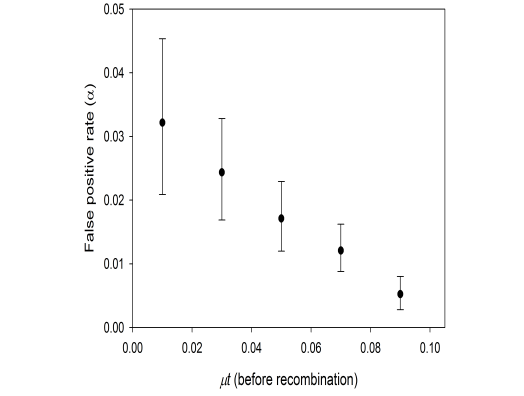
\includegraphics{Figures/HybridCheck/HC_FalseRate}
    \caption{\label{fig:HC_False}The mean($\pm$5 - 95\%CI) false positive rate ($\alpha$) of HybridCheck as a function of the ancestral divergence time $\mu t$ (i.e. the amount of time of the sequences diverged before recombination). As sequences become more diverged, the false positive rate decreases.}
\end{figure}

The false negative rate is presented in Figure~\ref{fig:HC_Power}. The false negative rate is plotted on the y-axis, against the amount of time since recombination occurred (expressed as $\mu t$). The data is partitioned into series, according to the amount of divergence (expressed as $\mu t$) between parental sequences prior to hybridisation. Figure n+1 shows that HybridCheck was able to detect $>$95\% of recent introgression events even if the two parental populations had diverged only moderately. However, more ancient introgression events were detected only if both parental populations had significantly diverged.

\begin{figure}
	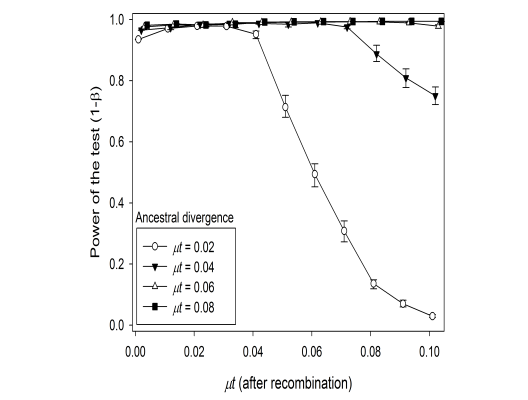
\includegraphics{Figures/HybridCheck/HC_Power}
    \caption{\label{fig:HC_Power}The mean($\pm$5 – 95\%CI) statistical power (1 - $\beta$) of HybridCheck as a function of the divergence time of the sequences after recombination (expressed in $\mu t$) for sequences with ancestral divergence times $\mu t$ = 0.2, 0.4, 0.6 and 0.8 generations. Recombination between moderately diverged sequences can be detected in $>$95\% of the cases, as long as the recombination event was relatively recent.}
\end{figure}

The accuracy of the dating estimates HybridCheck calculates for our simulated scenario is presented in Figure~\ref{fig:HC_Age}. This analysis shows that when the ancestral sequenced had diverged significantly ($\mu t \geq$ 0.2), the age estimates calculated by HybridCheck are a good approximation of the actual time passed since recombination (Linear Regression: Estimated age = 0.000795 + 0.968 t, R2=99.3\%). However, when the exchanges occurred between sequences that were only moderately diverged ($\mu t <$ 0.2), the age of the recombination events are underestimated when recombination happened in the distant past ($\mu t >$ 0.05) (see Figure~\ref{fig:HC_Age}). In such cases, mutations accumulated after the recombination event fragmented the blocks, resulting in an underestimate of the number of SNPs in the blocks that were detected.

\begin{figure}
	\includegraphics{Figures/HybridCheck/HC_Age}
    \caption{\label{fig:HC_Age}The mean ($\pm$SEM) estimated age (expressed in $\mu t$) of recombinant blocks calculated using the dating algorithm with a JC correction in HybridCheck, versus their actual age. In most of the scenarios, HybridCheck returns an unbiased estimate of the divergence time. However, the age is underestimated in cases of ancient recombination between populations that have ancestral divergence of 0.2.}
\end{figure}


\section{Discussion}
In this project, the objectives were to create and test a software package for the exploratory analysis of large sequences for evidence of introgression and hybridization. The package is designed to take the researcher through the following questions:

\begin{enumerate}
	\item Is there evidence of recombination / introgression?
    \item Where are the recombination regions in the sequences?
    \item What is the divergence time of recombinant blocks that are detected by the package?
\end{enumerate}

\subsection{Performance of detecting recombinant blocks}

The data demonstrate that for the simulated scenarios, HybridCheck performs best when sequences are diverged sufficiently prior to hybridization, and the hybridization or recombination event was relatively recent.
However, when the parental sequences of the hybrid sequence were sufficiently diverged recombinant blocks were clearly detected long after the recombination event ($\mu t >$ 0.06).
In addition, when divergence between parental sequences of a hybrid sequence was high then dating estimates of the recombinant blocks remained more accurate for older recombination blocks. 

If two parental sequences are significantly diverged prior to hybridisation, the introgressed regions will be more apparent in the sequence similarity scans of HybridCheck because their high nucleotide similarity stands in sharp contrast with the genomic background.
With a lower level of ancestral divergence, the increase in local sequence similarity caused by recombination is more difficult to distinguish from stochastic variation in nucleotide divergence, around a higher average level of sequence similarity.
As a result, the algorithm HybridCheck employs to decide on a suitable sequence similarity threshold can be confounded as it tries to identify regions with sequence similarity that fall outside of the mean noise levels of sequence similarity.
Therefore, HybridCheck would struggle to analyse a study system in which populations or taxa analysed are too closely related and have not diverged for long enough to accumulate unique polymorphisms which will be shared between parental and hybrid sequences. 

Previous studies have shown that many window based recombination detection methods perform better when the divergence is above ~0.05 (expressed as a proportion of the sequence length) \parencite{Posada2001b}.
Furthermore, simple implementations such as MAXCHI, and site incompatibility based methods usually perform better than phylogenetic based methods because the latter only tend to detect recombination if it changes the tree topology \parencite{Posada2001b}.

HybridCheck window scans attempt to find elevated similarity between genome sequences / contigs of two taxa which are unrelated.
Such elevations in similarity are indicative of, and often coincide with incongruence between differing gene tree topologies.
However, such signatures can have causes other than recombination, and elevated levels of sequence similarity could also be due to stabilizing selection conserving sequences between populations.
Alternatively, diverging populations of organisms could show increased levels of divergence in regions of the genome that are under adaptive selection, and if there is gene flow between populations the background will be homogenized compared to the regions that are subject to divergent selection \parencite{Nadeau2012}.
Such genomic islands of divergence appear to be less evident between populations that are further along the speciation process in butterfly species \parencite{Nadeau2012}.
A selective sweep is a phenomenon whereby positive selection in an allele reduces variation in neighboring regions due to linkage.
This is also called hitchhiking \parencite{Hedrick1980}.
If a selective sweep is strong and only one haplotype exists in high numbers in the population as a result, then a large reduction in variation is possible.
Selective sweeps could create regions of sequence similarity similar to those created by hybridisation events.
Note however, this scenario reduces variation around a positively selected allele within in a population.

HybridCheck attempts to overcomes these effects of selection in part by removing non-polymorphic sites prior to measuring the sequence similarity across sequences, but it is still possible that selection could be responsible, and the removal of informative sites by selection therefore reduces the power of HybridCheck to reliably identify introgression in those regions.
Therefore HybridCheck is not recommended or useful if a researcher is interested in smaller regions subject to very strong selection, due to the resulting lack of information.
If there are protein-coding regions in a detected recombinant region and selection is thought to be responsible, then the sequences should be analysed for evidence of purifying selection and/or selective sweeps within the detected region.

Elevated sequence similarity and incongruent tree topologies can also be caused by “incomplete lineage sorting” or deep coalescence \parencite{Rogers2014ComparativeDynamics}.
This occurs when an ancestral species is polymorphic for a given gene before the species tree splits into two daughter species.
After the first species split, if the polymorphism does not become resolved into two separate monophyletic lineages before the next speciation event, then the species tree will not match the gene trees of individual alleles \parencite{Rogers2014ComparativeDynamics}.
This problem is likely if a population size is very large, or if the time between branching events is low \parencite{Rogers2014ComparativeDynamics}.
Much of the genome of \textit{Homo sapiens} shows evidence of incomplete lineage sorting.
As a consequence, parts of the genome supported the phylogeny (chimpanzee, (human, gorilla)), whereas other regions of the genome supported the phylogeny (human, (chimpanzee, gorilla)) \parencite{Galtier2008}.
Both these phylogenies disagree with the species phylogeny of homonids (gorilla, (human, chimpanzee)) \parencite{Galtier2008,Rogers2014ComparativeDynamics}.
This discordance is because selection can cause similar sequences, or islands of divergence as previously described, and then incomplete lineage sorting results in gene trees that are discordant with the species tree and other gene trees, as a result of the incomplete and stochastic resolutions of polymorphisms, before subsequent speciation events \parencite{Scally2012}.

However, HybridCheck can help discern recombination from incomplete lineage sorting by comparing the coalescence time of recombinant regions with the split of the species.
If the age of a recombinant region is significantly younger than the split of the ancestral species, the pattern is inconsistent with incomplete lineage sorting.
In this case, genetic introgression after hybridisation is a more plausible explanation for the observed increase in local sequence similarity.
HybridCheck makes this practically possible for the researcher to do, for many recombinant blocks.

To summarise the performance of the HybridCheck when identifying recombinant regions, the HybridCheck use case is intended predominantly as an exploratory method to scan for signal between sequences from diverged populations or taxa, rather than within populations.
Outside of this use case, HybridCheck may be unsuitable for some systems as a result of limited divergence between sequences, and selection, both of which result in reduced information for the HybridCheck analysis method. 
Recent speciation and large population sizes may result in incomplete lineage sorting, which can affect patterns of divergence and ancestry in similar ways to recombination, however coalescent times computed by HybridCheck may help distinguish incomplete lineage sorting from recombination.
When using HybridCheck for a study system outside of its designed use case, whilst it is useful for highlighting the regions of the genome affected by the above factors, regions should not be uncritically considered the result of hybridisation or recombination, and the alternative causes e.g. selection should be followed up and ruled out before any such conclusion. 

\subsection{Performance of estimating the age of recombination events}
From the results it is evident that the dating algorithm used in HybridCheck tends to underestimate the divergence time of recombinant blocks in old recombination events. This is because recombination blocks can become fragmented by accumulation of subsequent mutations following the recombination event. Consequently, older recombination blocks tend to be smaller, when they are actually larger. Thus, not all mutations are accounted for, resulting in an underestimate of the divergence time particularly for old recombination events.

Furthermore, the dating algorithm used in HybridCheck makes several assumptions in order to be simple and fast. As a result however, if these assumptions are broken then this will affect how representative the estimates returned by HybridCheck are of the true age of a recombination event. The algorithm assumes that the mutation rate has been constant over time and identical in all taxa. This assumption is not always true, and more sophisticated approaches, such as the Fossilized-Birth-Death process allow for the calibration of divergence time estimates during Bayesian phylogeny estimation \parencite{Heath2014}. It uses all available fossils, and considers extant species and fossils of species part of the same macro-evolutionary process \parencite{Heath2014}.

In addition, the algorithm uses a nucleotide substitution rate to infer the mutation rate. In order to correct for mutation saturation, homoplasy, back mutations and transition / transversion ratios, HybridCheck converts the number of SNPs into the number of mutations using a JC \parencite{Jukes1969}, K80 \parencite{Kimura1980ASequences}, F81 \parencite{Felsenstein1981EvolutionaryApproach}, HKY \parencite{Hasegawa1985DatingDNA}, or GTR \parencite{Tavare1986SomeSequences} correction. However, substitution rates do not solely depend on mutation rates, and they appear to be auto-correlated across sequences due to the effect of selection. Selection can vary between sites, genes and taxa, and selection and substitution rates can change through time as conditions change \parencite{Barrick2013,Bromham2003a}.

Furthermore, the size of populations must be taken into account \parencite{Bromham2003a}. Bayesian coalescent approaches incorporated in software such as BEAST \parencite{Bouckaert2014BEASTAnalysis} should be used when using a relaxed clock or more advanced method of dating. However, these methods are computationally more demanding and might become unfeasible when estimating the divergence time of a large number of recombination events. In such cases, the age estimate returned by HybridCheck offers a good approximation when recombination occurred relatively recently ($\mu t <$ 0.05), and also when the ancestral sequences have diverged significantly before hybridizing.

In conclusion, the HybridCheck project is intended as a simple all-inclusive tool to analyse recombination in genome sequence data. The implemented algorithms are not as sophisticated as methods that employ Bayesian estimation of parameters and coalescent simulations. However, this means that the package is computationally fast, which makes it a useful first port-of-call for identifying recombination and assessing whether other explanations such as incomplete lineage sorting may apply.

\setcounter{chapter}{2}
\chapter{The role of introgression in the adaptive evolution of the generalist plant pathogen, \textit{Albugo candida}}
\label{chap:Acandida}
\chaptermark{Evidence of hybridisation in \textit{Albugo candida}.}

This chapter is based on the published scientific paper:

\vspace{5mm}

\textit{McMullan, M., Gardiner, A., Bailey, K., Kemen, E., Ward, B. J., Cevik, V., ... Jones, J. D. (2015). Evidence for suppression of immunity as a driver for genomic introgressions and host range expansion in races of Albugo candida, a generalist parasite. eLife, 4, 1-24.}

\vspace{5mm}

This thesis chapter presents a research project that was a collaboration between many researchers.
In this chapter in order to provide clear description of the work involved, some details regarding some work that has not been performed by myself are presented.
Specifically, work described in sections 3.2.1 and 3.2.2 were completed by collaborators and not myself.
My contributions to the work are described in sections 3.2.3 and 3.2.4, and it is results of this work that is presented in this chapter.


\newpage


\section{Introduction}
Host specificity is a defining feature of pathogens, and can be defined as the inverse of the number of hosts that a given pathogen can infect \parencite{Poulin2008}. Host specificity is negatively correlated to the probability of parasite extinction, and positively correlated to the ability of a parasite to colonise and adapt to a new host \parencite{Poulin2008}. Host specificity is constrained by the physiology of the pathogen. Therefore the host specificity of a pathogen is constrained by factors including (but not limited to) the pathogen's method of transmission, method of obtaining nutrients and energy from the host, and the ecology of the pathogen and host \parencite{poulin2011evolutionary}. Such factors are proximal constraints on host specificity, but host specificity is ultimately constrained by the evolutionary and biogeographical history of the pathogen and its potential hosts \parencite{Poulin2008,poulin2011evolutionary}.

A highly specialist parasite occurs in only a single host species. They often require host-host contact for transmission, and their longevity and future is strongly linked to that of their host species \parencite{Poulin2008}. Conversely, a parasite that is more generalist may survive the extinction of one host species, since there is another host species they can exploit to survive. Generalist parasite species may rely less on contact-transmission or close proximity between hosts. For example, they may be transmitted through food, or some other species vector \parencite{Pedersen2005PatternsPrimates}. However it should be noted that even if a pathogen has a very high mobility, and dispersal, its host-specificity can be high \parencite{Poulin2008}.

The availability of ecologically and evolutionarily related or similar hosts cohabiting the same habitat, may cause differences in the host-specificity of two otherwise similar pathogen species \parencite{Jex2006TheSpecificity.}. Furthermore, parasites put selective pressure on host populations to adapt and develop immunity, increasing the frequency of genetic and epigenetic variants that improve immunity, and pathogen detection in the host. As a result, these adapting host populations impose selection pressure on the pathogen populations, increasing the frequency of variants that maintain the pathogens efficiency of immune suppression. Over time, both host and parasite co-evolve and become intimately associated, as they both adapt to each other's latest antagonistic evolutionary innovations. This is called an evolutionary arms-race \parencite{Boutemy2011,Buckling2002,Cooper2008,Kemen2012,Lamour2010}.

Overall, the general pattern observed in nature, is that most parasite species are largely specialised and co-evolve with only a few, if not one, host species \parencite{McMullan2015a}. It should be noted however, that this generalisation is based on a measure of host specificity that is based on a simple measure of host specificity, namely the number of host species that are colonised by a parasite in natural populations. However this metric makes an oversimplification that does not reflect biological reality. For example, two pathogen species may have the same number of host species, but if one of the pathogens infects species of one genus, and the other infects species of multiple genera, then it is not realistic to conclude both of the parasite species are equally specialised. It is because of this problem, that \cite{Poulin2003ParasiteSpecificity} defined a host-specificity measure that takes into account the taxonomic or phylogenetic distances between the hosts colonised by a parasite. Later the authors published an improved metric that incorporated the phylogenetic or taxonomic distinctness of a pathogens host species, but also weighted for the prevalence of the parasite on its different host species \parencite{Poulin2005CombiningSpecificity.}⁠. The rationale for such a weighting is that a pathogen that is largely concentrated on only one of its multiple hosts should be classified as more specialised than a pathogen that utilises and colonizes all of its host species evenly.

The organism of interest in this work is the obligate biotrophic plant pathogen, \textit{Albugo candida}. Plant pathogens have a parasitic relationship with their host, and are classified according to the nature of this relationship with the host. Pathogens which obtain nutrients from decaying plant matter are classified as necrotrophs, whereas pathogens which require living host tissue in order to obtain nutrients are classified as obligate biotrophs \parencite{Kemen2012}⁠. These biotrophs don't typically secrete abundant lytic enzymes, and cause little physical or structural damage to the host plant \parencite{Kemen2012}⁠. Pathogens with a combination of these two lifestyles are classified as hemibiotrophic \parencite{Kemen2012,Lamour2012PathogenCapsici}. \textit{Albugo candida} is an obligate biotroph, and whilst \textit{Albugo candida} is a generalist, infecting species of the Brassica family, obligate biotrophs are typically specialists \parencite{McMullan2015a}⁠.

After an obligate biotroph makes a host-jump, it is expected that selection will increase any adaptive genetic or epigenetic variant in the population that results in more efficient immune suppression of the new host \parencite{Dong2014,Kemen2012,Poulin2008,Raffaele2010,Thines2014}. Furthermore, host-parasite co-evolution over time will result in both the host and parasite constantly adapting to each others latest antagonistic adaptations, and they will become more intimately associated historically \parencite{Morgan2007,Raffaele2012,Thines2014}. As both of these processes occur, new effectors and pathogenicity factors may be created, and existing ones may receive beneficial mutations, and they may also have their levels of expression changed epigenetic modification and inheritance \parencite{Dong2014,Gijzen2014EpigeneticPathogens,Raffaele2012,Raffaele2010,Win2012}. These will be fixed due to selection pressure if they are beneficial. These modifications enable more efficient immune suppression and exploitation of one host species, but increase the risk of detection in other host species by triggering their immune system \parencite{Martin2012EffectorsInteractions}. Thus, as obligate biotrophic pathogen populations become more adept at suppressing the immunity of one host, they will become less adept at infecting previous host(s) or other hosts it can infect.

Therefore, obligate biotrophs are typically known for being intimately associated with their hosts i.e. they have a high host specificity \parencite{Thines2014}. Yet there are generalist biotrophic parasites that appear to have overcome this evolutionary dilemma and show virulence on diverse hosts. \textit{Albugo candida}, the organism that is the subject of this work, is one such generalist, but there are other generalist oomycetes, like \textit{Phytophthora capsici} \parencite{Lamour2012PathogenCapsici}⁠.

Some generalist parasite species have solved the dilemma by evolving multiple specialised races, and each specialised race can infect a different host. For example, the eukaryotic order \textit{Albuginales}, of which \textit{Albugo candida} is a member, is completely comprised of obligate biotrophic pathogens that cause disease on a broad range of plant hosts \parencite{Biga1955ReviewConidia.,Choi1955,Walker2007AHost.}.

Albugo is the largest genus of the order \textit{Albuginales}, and it was reported to consist of 33 specialist pathogens by \cite{Biga1955ReviewConidia.}⁠. More recently, the estimate is that the genus comprises approximately 50 pathogens, and these are typically specialists. In addition new distinct \textit{Albugo} species have been discovered that were previously thought to be members of \textit{Albugo candida} (Pers) Roussel. \parencite{Choi2011,Choi2009,Ploch2010,Thines2009}. This is because in the past decades, classification was based largely on morphology, and this led to the application of a broad species concept, that resulted in \textit{Albugo candida} (Pers.) Roussel being regarded as the causal organism of all incidents of white blister rust on all \textit{Brassicaceae} hosts \parencite{Choi2011}. As late as 2011, it has been estimated that “a dozen” distinct species thought to be \textit{Albugo candida} await discovery \parencite{lamour2009oomycete}.

\textit{Albugo candida} (Pers.) Roussel can infect 241 species of plants in 63 genera from the families of \textit{Brassicaceae}, \textit{Cleomaceae} and \textit{Capparaceae} \parencite{Choi2009}⁠. \textit{Albugo candida} infections are the causal agent of white blister rust disease, resulting in significant losses on \textit{Brassica} crops of economical importance. For example, \textit{Albugo candida} causes  up to 56 of yield losses in Indian Mustard \parencite{Meena2002YieldSeverity}. \textit{Albugo candida} consists of different “physiological races”, each usually featuring high host-specificity and approximately 24 races of \textit{Albugo candida} have been defined, based on their host range \parencite{saharan2014white,Saharan1992WhiteSpecies}.

\textit{Albugo candida} reproduces both asexually and sexually \parencite{Holub1995}⁠. During asexual reproduction, diploid zoospores are formed in zoosporangium beneath the leaf epidermis. The zoosporangium are visible when dehydrated and in large numbers, as white blisters \parencite{Holub1995}. These sporangia then rupture the epidermis of the host leaf, to release zoospores for dispersal. During sexual reproduction, fertilization between two isolates creates non-motile, diploid, and thick-walled oospores \parencite{Holub1995}⁠. The oospores can resist extreme temperatures and desiccation. The relative importance of both reproductive modes is not well established, but the clonal (asexual) mode of reproduction allows rapid population expansion, especially given modern crop mono-culture growing practices. Although \textit{Albugo candida} comprises distinct, specialised physiological races that colonize different host plants, and that distinct species have been identified that were initially thought to be \textit{Albugo candida} \parencite{Choi2011}, it is still considered a single species.

According to evolutionary and population genetic theory, the trade-offs associated with adaptation and host-specialisation, coupled with strong population structuring, can result in adaptive radiation and speciation \parencite{Abbott2013,Stukenbrock2013EvolutionPathogens}. \textit{Albugo candida} then may be thought of as a currently ongoing adaptive radiation; The broad host range of \textit{Albugo candida} is enabled by an ongoing specialisation of independent physiological races, and these races are likely heading for speciation \parencite{Dres2002a}. If strains or races of a parasite develop adaptations to specific hosts, and make trade-offs in doing so, specialising to the given host, does parasite specialization inevitably lead to speciation? Certainly, specialising on one or a few hosts, at the cost of being able to infect other hosts, will mean separation of specialised races, ecologically, and even geographically, over time such separation is expected to result in  reproductive isolation.

Compared to other microbial plant pathogens, \textit{Albugo} species are notable as infections strongly suppress host innate immunity. As a result, infections of \textit{Albugo} species increase the susceptibility of the host to a secondary infection by pathogens that would otherwise be avirulent, including downy mildews \parencite{Cooper2008}. It has been suggested that this immune suppression caused by \textit{Albugo} infections might allow an accelerated adaptation of other pathogen species to host that is susceptible to \textit{Albugo} species \parencite{Thines2014}⁠.

However, whilst it has been suggested the immune suppression will accelerate the adaptation of other pathogens to the suppressed host, before this project, no evolutionary rationale was proposed explaining why rendering a host susceptible to other pathogens could be adaptive for the various Albugo species. Hypothetically, a pathogen which colonizes and adapts to the hosts of Albugo species due to the immune suppression of Albugo species infections, will become competition against Albugo species for the same resources \parencite{Cooper2008}⁠.

Suppression of host innate immunity would facilitate cohabitation of distinct physiological races that otherwise would not come into contact due to their specialisation and adaptive trade-offs, as previously discussed. When the distinct physiological races come into contact, genetic exchange including introgression and hybridisation may occur between them. Here, introgression is defined as the introduction of nucleotide variation from a parental donor race into the genome of a recipient race, through the mechanism of recombination \parencite{Hedrick2013}. This flow of genetic variation from one donor physiological race, to a recipient physiological race, could slow down the genetic divergence of the races, and slow or prevent speciation. However, introgression between races that are specialised and adapted to exploit different hosts could be maladaptive, and therefore could be strongly selected against. This is because hybrids would inherit effector alleles derived from both parental races. Therefore, whilst the hybrid genomes would contain effectors that enable the immune suppression of multiple hosts, they could also contain effectors that trigger immunity on multiple hosts. Immune recognition of even a single effector is sufficient to trigger the immune response and stop an infection. Therefore any hybrid that possess an expanded repertoire of effector alleles are likely to have a strong fitness disadvantage on most potential host plants, as with larger effector repertoire's comes an increased likelihood of one of them triggering host immunity.

This chapter presents work conducted and contributed to a larger genome project analysis of \textit{Albugo candida}, conducted by a team of scientists at the University of East Anglia, and The Sainsbury Laboratory. This project aimed to answer the following questions, in order to try and resolve this question of whether immune suppression and secondary infection is adaptive or maladaptive, and whether it is due to hybridisation:

\begin{enumerate}
\item Are the distinct physiological \textit{Albugo candida} races genetically isolated and ‘on the road to speciation’?
\item Does suppression of host innate immunity enable cohabitation and growth of races with non-overlapping host ranges?
\item Are the genomes of \textit{Albugo candida} affected by recombination and hybridisation?
\end{enumerate}

The work presented in this chapter was primarily conducted with a goal of answering the third question of the project. During the collaborative project, genome sequence assemblies were created for five isolates that were collected from four host species (\textit{Brassica oleracea}, \textit{Brassica juncea}, \textit{Capsella bursa-pastoris}, and \textit{Arabidopsis thaliana}). This chapter presents analyses performed on the assembled sequence scaffolds for the detection of recombination, hybrididation, and mosaic genome structure.


\section{Methods}
In order to perform the analysis of genome structure that is the focus of this chapter, prior work was conducted to isolate the \textit{Albugo candida} races used in this study, test for virulence, extract and sequence DNA, and RNA, and perform genome and transcriptome assemblies. These procedures are subsequently described in detail in \parencite{McMullan2015a}, and given that these procedures are not the focus of this chapter, the reader is referred to this paper for details on the wet lab and molecular methods. A brief summary of these methods is described below.

\subsection{Isolation and cultivation of races used in the study}
In order to address the research questions presented in the previous section, genome sequence assemblies were required of five isolates of \textit{Albugo candida}, the white rust fungus. These isolates were collected from four different host species: \textit{Brassica oleracea}, \textit{B. juncea}, \textit{Capsella bursa-pastoris}, and \textit{Arabidopsis thaliana}. The isolates were collected by Erik Kemen, prior to the evolutionary analyses that are the focus of the present chapter. 

The isolate designated AcNc2, was isolated from infected leaves of \textit{Arabidopsis thaliana} Eri-1 field-grown plants in Norwich, England. The isolate was collected in 2007. The isolate AcEm2 was collected from wild \textit{Capsella bursa-pastoris} in Kent, England in 1993. AcBoT was collected from infected cultivars of \textit{Brassica oleracea} called 'Bordeaux F1', from Lincolnshire, England, in May 2009. AcBoL was harvested from infected \textit{Brassica oleracea} leaves from Lincolnshire, but in the January of 2009. An isolate which is virulent on \textit{Brassica juncea} called Ac2V was provided by M Borhan of Agriculture and Agri-Food, Canada. All of these isolates were single spore purified \parencite{Kemen2011}.

\subsection{Genome assemblies of isolates}
The assembly of isolate AcNc2 was used as a reference. The assembly is 34Mb in size, and has 5212 contigs of approximately 160-fold coverage. The assembly was approximately 73\% of an estimated genome size of 45Mb. The unassembled part of the genome (approximately 11Mb) is likely to contain repeats, approximately 8\% of which represent collapsed regions, since they have coverage that is several times higher than the average. For each isolate, several assemblies were constructed with different k-mer lengths. Each assembly was assessed according to number of contigs, N50 (Bp and number), mean contig length, assembly size, GC content, average genome coverage, repeat content, and the number of predicted genes. High sequence similarity of the five \textit{Albugo candida} isolates resulted in the conclusion that three races had been sequenced: AcNc2, and AcEm2 were isolates of the same race, and AcBoT and AcBoL were also two isolates which belonged to the same race. Therefore, detection of recombination and hybridisation in this chapter were first conducted on the three races AcNc2, Ac2V, and AcBoT, each of which had a 33-34Mb assembly.

\subsection{Detection of recombination events}
Recombination events were statistically identified on contigs $\geq$10,000 Bp using the software RDP3 using five independent detection algorithms: RDP \parencite{Martin2000RDP:Sequences.}, GENECONV \parencite{Padidam1999PossibleRecombination.}, Maxchi \parencite{Smith1992a}, Chimaera \parencite{Posada2001b}, and 3Seq \parencite{Boni2007AnTriplets}. All of these tests are available in the Software Package RDP for Microsoft Windows \parencite{Martin2015RDP4:Genomes}. Tests were conducted using a critical value α = 0.05 and p-values were Bonferroni corrected for multiple comparisons of sequences. Sequences were made linear using unphased base calling, i.e. where a sequence has a base position that is heterozygous, one of the nucleotides was assigned at random at that site. 

Recombination events were only considered genuine if they were supported by at least three of the recombination detection methods in RDP, and recombination events detected using the methods in RDP were only counted if the parental sequences could be identified, and the start and end positions of recombination events were unambiguous.

In order to visualise the effects of recombination and hybridisation on the genome structure of the \textit{Albugo candida} races, the software package HybridCheck was developed for the R programming language. The development and testing of this software package is described in detail in chapter \ref{chap:HC}, so only a brief description will follow. HybridCheck can analyse three sequences with a sliding window scan, and produce plots with use the RGB tricolour system to indicate where regions of hybridisation or recombination have occurred between sequences. Each sequence is designated one of the three primary colours, red, blue, or green. In regions of a given sequence that are unique, then those regions are coloured in with the unique colour of that given sequence. However, in regions of the sequences in which all the SNPs are shared with another sequence, then the region is coloured with the “hybrid” colour of the two sequences (e.g. yellow if the two sequences have the unique colours red and green). All monomorphic sites are excluded in this computation. In cases where recombination is recent, the hybrid colouration is strong as most of the SNPs are shared between two sequences. However older events may have accumulated mutations since the recombination / hybridisation event. In such a case, there are less shared SNPs between two sequences, and the colour intensity is less strong.

\subsection{Dating identified recombination events}
Immediately after a recombination or hybridisation event has occurred, a hybrid or recombinant offspring's DNA sequence will have regions which are near identical to one parent, and regions which are near identical to the other parent. In those regions the molecular clock is effectively zeroed. Therefore, for a given recombinant region, the only substitutions which could be observed between the recombinant and the donor must have occurred since the recombination event took place.

This divergence between a donor sequence region, and the same region in the recombinant offspring was used to estimate the time since the recombination event. Two methods were used to calculate the number of generations since individual identified recombination events occurred. A binomial mass function was used, which was developed for the HybridCheck R package. The equations are described more fully in chapter \ref{chap:HC}. Briefly, the method computes a window of time, within which the recombination event is most likely to have occurred. It does this by taking into consideration the cumulative probability of observing the number of mutations that have occurred in the recombinant region, between donor and parent, given the average mutation rate. The function assumes that the recombination event has evolved neutrally since the recombination event occurred, and that mutation rates between the two sequences were constant through time, and equal in both sequences. The mutation rate in oomycetes is unknown, and therefore the binomial mass function was used with two different mutation rates: μ = 10−6 and 10−7 per base per generation. This binomial mass function was used to analyse all detected recombination events.

In addition to the binomial mass function, an analysis was conducted in BEAST \parencite{Drummond2007BEAST:Trees}. Phylogenetic trees were estimated with a HKY + G model, a Yule tree prior, and a strict molecular clock assumption, where the mutation rate was assumed to be $\mu = 10^{−6}$. Ten independent analyses were run, with an MCMC of 10 million steps, with a burn-in of 10\%. Because of the computational complexity and time required for BEAST analyses, 20 recombinant regions were analysed in this manner. The results were compared to the date that was estimated for the recombinant region by the binomial mass function, and this confirmed that the binomial mass function provides a good approximation of the divergence time.


\section{Results}
\subsection{Distribution of polymorphisms across races}
Polymorphisms were found to be unequally distributed across the genomes of the \textit{Albugo candida} isolates analysed. In some regions of the genome, there are stretches of identical sequence which are as long as 10kb in length. In other regions of the genome, stretches of lower sequence similarity may be found. For example, between the isolates AcBoT and AcNc2, a region of approximately 5kb was observed with 89\% sequence similarity. This is demonstrated in Figure \ref{fig:AC_Res_1}.

\begin{figure}
\includegraphics{Figures/AlbugoCandida/AC_Figure1}
\caption{Nucleotide identity amongst the homologous genomic regions of Ac2V, AcBoT and AcNc2. The mean identity was calculated for the sliding window of 20 Kb.\label{fig:AC_Res_1}}
\end{figure}

The distribution of the polymorphisms is highly suggestive of a mosaic-like genome as the polymorphisms are not only distributed unevenly, but they were distributed in a block-like manner.
Stretches of nucleotide similarity are arranged in a block like structure; there are regions where AcNc2 is highly similar to AcBoT (and therefore diverged from isolate Ac2V), followed by regions where isolate AcNc2 is highly similar to Ac2V (and therefore diverged from isolate AcBoT).
The HybridCheck software package visualises such genome structure in Figure \ref{fig:AC_Res_2}. The figure visualises the effect on the genome by colouring regions yellow where races AcNc2 and AcBoT show near sequence identity, cyan where races AcBoT and Ac2V show near sequence similarity, and purple where races AcNc2 and Ac2V show near sequence similarity.
Note that in the figures, there are also regions of unique colouration (red, green, and blue), and such regions represent diverged parts of the genome where the three races have large proportion of unique (races-specific) polymorphisms (Figure \ref{fig:AC_Res_2}).

\begin{figure}
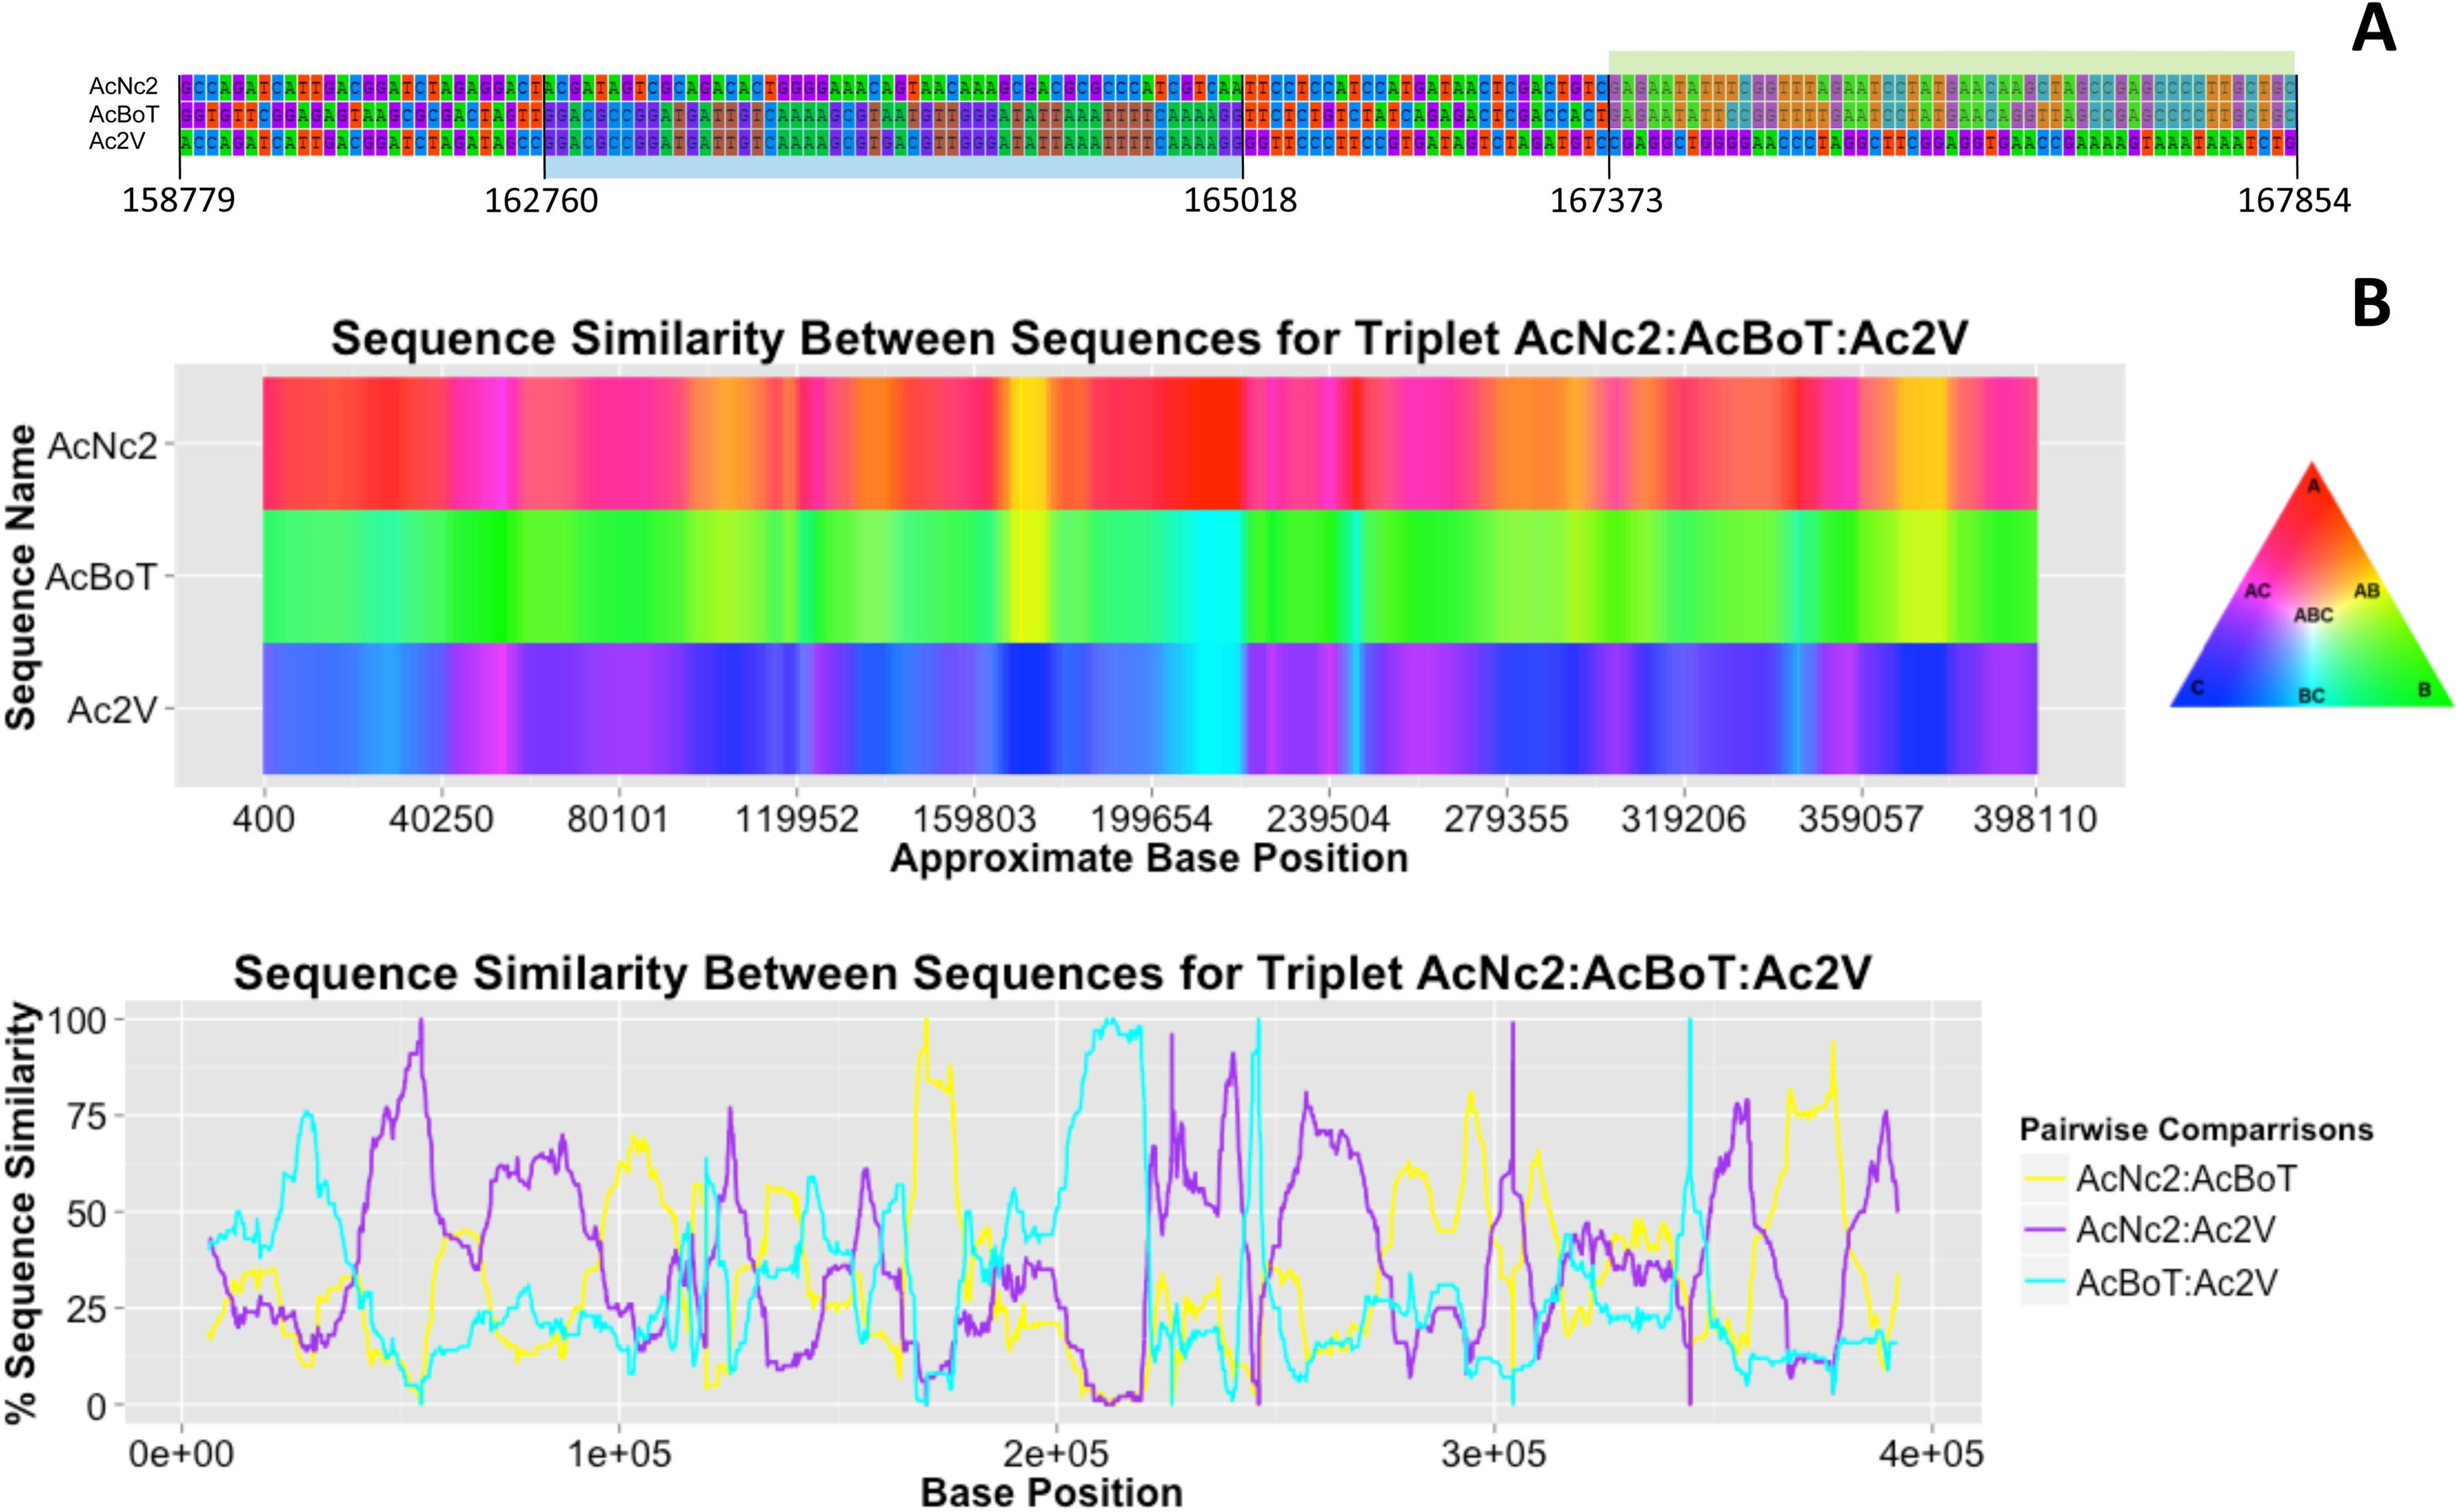
\includegraphics{Figures/AlbugoCandida/AC_Figure2}
\caption{Extensive variation in sequence similarity between \textit{Albugo candida} races.
\textbf{A)} An sequence alignment between base positions 158,779 and 167,382 within contig 1 of \textit{A. candida} races AcNc2, AcBoT and Ac2V. Two recombination blocks coloured blue and green are visible, displaying high sequence similarity between races.
\textbf{B)} The sequence similarity across the length of contig 1, amongst three \textit{A. candida} races. Similarity is visualised using the colours of a RBG colour triangle in the software HybridCheck. Areas where two contigs have the same colour (yellow, purple or turquoise) are indicative of two races sharing the same polymorphisms. The linear plot of the proportion of SNPs shared between the three pairwise comparisons between the races. Shown on the X-axis is the actual base position.\label{fig:AC_Res_2}}
\end{figure}

This observation of alternating blocks of high sequence identity between otherwise diverged (as represented by areas of red, green, and blue) genomes, provides supporting evidence for genetic introgression between diverged races that show a considerable (yet still incomplete) level of reproductive isolation. The recombination detection methods described in the previous section test for recombination blocks visualised here, formally.

\subsection{Recombination blocks identified using RDP}
All 133 contigs were analysed for presence of recombination blocks using algorithms in the software package RDP.
Recombination analysis with these algorithms identified ~675 recombination blocks on 127 sequence contigs which were significant, even following correction of the alpha with a Bonferroni correction.
These identified blocks were reported as significant for at least three different recombination detection tests.
If the length of all the significant blocks is summed in a linear fashion, then approximately 25\% of the total length of all contigs analysed is identified as recombinant, this is equal to 3Mb.
These blocks represent regions of the genome which are derived from either another race, or the ancestor of another race.
Algorithms in RDP were able to report such donor sequences in some cases. 
The full data-set from the RDP output is publicly available from http://dx.doi.org/10.7554/eLife.04550.015.

\subsection{Estimated ages of recombination events}
Dating analysis of the significant recombination blocks using the HybridCheck binomial algorithm indicated that the recombination events detected occurred at a range of different dates. If one assumes a $\mu = 10^{-8}$ substitution rate which is constant across cell cycles, and that there are 100 cell cycles per year, then the most recent introgression event occurred approximately 220 years ago, and the oldest detected event occurred almost 200,000 years ago. The mean age for all the detected recombination events is approximately 6237 years ago, with a standard error of 12,594 years. Furthermore, there is no significant difference between the average estimated dates across different contigs.

The wide range in age estimates of the introgressed regions provides evidence for the hypothesis that recombination and hybridisation between diverging \textit{Albugo candida} races has been a consistent and ongoing evolutionary process, affecting the entirety of the genome. This finding rules-out the hypothesis that one or a few recombination/hybridisation events in the distant past are responsible for creating the mosaic structure observed. This also helps explain the cause of the mosaic genome structure that has been observed: occasional introgression events across a range of evolutionary times is expected to result in genome containing introgressed blocks of sequence from a donor race, interspersed inside the distinct genomic background of the recipient race (i.e. the very pattern observed in \textit{Albugo candida}).

\begin{figure}
\centering
\includegraphics[width=0.7\textwidth]{Figures/AlbugoCandida/AC_Figure3}
\caption{\textbf{A)} Age of the 675 recombination blocks, identified across the whole genome, estimated using the HybridCheck binomial mass function, assuming a substitution rate of $\mu = 10^{−6}$; \textbf{B)} A box plot of the median (plus first nation blocks and third quartile) log-age of recombination events in contigs. Only contigs with eight or more events are shown. There is no significant difference in age of events between contigs (GLM: $F22, 233 = 1.06$, $p = 0.387$).\label{fig:AC_Res_3}}
\end{figure}


\section{Discussion}

The genome of \textit{Albugo candida} appears to have a mosaic-like genome structure: 675 regions were identified in 127 analysed contigs, which were consistently identified by multiple and independent recombination detection methods. 
The mosaic-like structure reflects discordant phylogenetic signals of genomic regions with distinct coalescence, and this suggests that introgression has occurred at a range of time points throughout the evolutionary history of the \textit{Albugo candida} races.

\subsection{Hybridisation and clonal reproduction of \textit{A. candida}}

\textit{Albugo candida} is an obligate biotroph, growing and reproducing on living plant tissue, and virulence experiments confirm that the \textit{Albugo candida} races isolated in this study are indeed host specific \parencite{McMullan2015a}⁠.
To explain the observed mosaic genomes, two distinct and host specialised \textit{Albugo candida} races would have to make contact by colonizing the same host plant in order to hybridize, although ex-situ hybridisation cannot be ruled out. 
Yet, any \textit{Albugo candida} race landing on a non-host plant is likely to trigger host immunity before it can mate with another distinct race.
So, given that the genome structure expected from recent introgression between distinct races is observed, how have they made contact?
One potential explanation was that infected host plants could form secondary contact zones for \textit{Albugo candida}: if a host plant was infected by a compatible (infectious) \textit{Albugo candida} race its immunity would be suppressed.
With a suppressed immune system, non-specialised \textit{Albugo candida} races might be able to colonise the already infected host, enabling both races to make contact and hybridise through sexual reproduction.
This hypothesis was tested with experimental infections of host plants with multiple races.
These experiments confirmed that a virulent race of \textit{Albugo candida} could suppress the immunity of its host plant, such that other non-virulent races of \textit{Albugo candida} could co-colonise it \parencite{Cooper2008,McMullan2015a}.

Following formation of a viable hybrid, clonal reproduction would allow fast dispersal of the pathogen and population expansion.
This aspect of the model was supported by analysing genomic identity between isolates which infect the same host species (i.e. within different races) and quantifying the shared proportion of heterozygous sites.
Genotypic similarity at heterozygous sites of pairs of independent isolates that infect the same host plant was exceptionally high; AcBoT and AcBoL shared 97\% of their heterozygous sites in common, and AcEm2 and AcNc2 shared 99.95\%.
Sharing of this proportion of heterozygous sites rules out Mendelian segregation and sexual reproduction, and confirms that these isolated were reproduced clonally. 
Given that AcEm2 and AcNc2 were sampled 100 miles apart geographically, and ten years apart in time, clonal reproduction appears to be the principal mode of reproduction of this race of agronomically important pathogens. 

The largest contig of the reference assembly, (contig 1; ~400kb) was used to analyse polymorphism distribution and detect recombination blocks.
The proportion of heterozygous sites in contig 1 was calculated for each isolate. 
Very few sites of contig 1 were heterozygous within AcNc2 (0.03\%), AcEm2, and Ac2V (0.01\%).
Within isolates AcBoT and AcBoL, the proportion of heterozygous sites was higher (both 0.65\%).
The high levels of genotypic identity observed between isolates which infect the same the host species would not be expected if sexual reproduction and Mendelian segregation was the primary mode of reproduction, especially given that isolates AcEm2 and AcNc2 are separated by approximately 100 miles and 10 years.
Furthermore, the high proportion of heterozygous sites (for contig 1) in isolates AcBoT and AcBoL is more consistent with asexual population expansion: A diploid organism reproducing asexually/clonally most of the time will accumulate mutations between each pair of homologous chromosomes.
This will generate more heterozygous sites over time, resulting in allelic divergence and increased observed heterozygosity.
However, the observation of a low level of observed heterozygosity in AcEm2 and AcNc2 is not expected in organisms where asexual and clonal reproduction is the primary method of reproduction.
Given there is no evidence of self-fertilisation (or any other form of asexual reproduction), it is likely that gene conversion has been operating to reduce within genome diversity in the races over time.
The phenomenon is called Loss of Heterozygosity or LOH, and it has been observed in other plant pathogen species such as \textit{Phytophthora capsici} \parencite{Lamour2012PathogenCapsici}⁠, as well as at a whole genome scale in yeast \parencite{Diogo2009}.
In both studies it was hypothesized the Loss of Heterozygosity observed has facilitated rapid adaptive evolution and genome plasticity.

To summarise, it appears that the generalist pathogen \textit{Albugo candida} is comprised of distinct physiological races, which are diverging as they specialise on different host species.
Secondary contact between distinct races on an immunosuppresed hosts results in inter-specific sexual reproduction between races, producing new hybrid offspring. 
These hybrids may be able to spread rapidly by clonal reproduction on their own, or introgression may occur.

\subsection{Biology of genetic introgression and hybridisation}
Introgression is defined as the transfer of genetic information (DNA or RNA) from one species (or OTU, race, or biotype) to another as a result of hybridization between them followed by repeated backcrossing \parencite{Ridley2004,Abbott2013}.

Hybridisation and introgression can lead to a mosaic-like genome structure, with regions of different parental lineages interspersed throughout the genome \parencite{Baack2007,Stukenbrock2012}.
Those regions will have different ancestry or coalescence, and hence, be represented by different phylogenetic trees.
Introgression has the potential to augment the adaptive evolutionary potential of populations and introduce a source of genetic variation into genomes.
As a source of genetic variation, mutations have longer waiting times, and lower initial frequencies.
In contrast, introgression can occur multiple times, thereby increasing the probability of fixation of the variant.
Furthermore, whereas mutations tend to be neutral \parencite{Kimura1968EvolutionaryLevel.}, or have (slightly) deleterious fitness effects \parencite{Ohta1973}, introgression inserts “pre-selected” variation of one of the parental (donor) lineages into the hybrid line \parencite{Hedrick2013}.
Adaptive introgressed variants can be new, have less pleiotropy, less strong linked effects, and less recessivity \parencite{Hedrick2013}⁠.
In contrast to mutation, multiple simultaneous changes across multiple loci are possible with hybridisation and introgression, but whether these multiple changes are deleterious or not depends on the details of the molecular interactions within the hybrid.

The view of Wright is that selection favours favorably interacting gene combinations, resulting in a highly integrated genome which contains coadapted gene complexes \parencite{Wright1931,Wright1932TheEvolution,dobzhansky1970genetics}. However, Fisher argued that selection acts on individual genes, and would favour genes which increase fitness on average across all possible genetic backgrounds of a given lineage, such genes were called "good mixers" \parencite{Fisher1930THESELECTION}. Both of these views are compatible with the concept of negative epistasis \parencite{Hedrick2013,Burke2001GeneticsHybrids} in a hybrid genetic background (also called hybrid incompatibility): In any two separated lineages, fixation of alleles in one lineage occurs independently and there is no selection for compatibility with any other lineage. Hybridisation produces novel genotypes which have not previously been subject to selection, and if they are less well adapted than the parental genotypes, selection would act against such less fit hybrids. This reduction in fitness of segregating hybrids has been taken as evidence for unfavorable interactions between genomes of parental individuals, negative epistasis, and hybrid incompatibility. The most widely accepted model of such incompatibility was developed by Bateson, Dobzansky and Muller \parencite{Dobzhansky1936StudiesHybrids.,Muller1942IsolatingTemperature}. Negative epistasis has been confirmed empirically in several animal and plant organisms in the past, including (but not limited to) \textit{Drosophila spp.} \parencite{True1996,Palopoli1994GeneticsStudies,Hollocher1996TheEffects,Cabot1994GeneticsSterility}, \textit{Helianthus spp.} \parencite{Rieseberg1996,Rieseberg1999HybridSpecies}, \textit{Tigriopus californicus} \parencite{Burton1990HybridApproach,Burton1990,Burton1999GeneticComplexes}, and \textit{Iris spp.} \parencite{Cruzan1994AssortativeZone,Burke1998GeneticHybrids}, and is a primary cause of hybrid inferiority.

However, hybrids can be superior to their parental lineages. Hybrid fitness can occur by several means. F1 hybrids are commonly larger in body size and have higher growth rates and yields \parencite{Baack2007,Hedrick2013,Burke2001GeneticsHybrids}. Such vigour is called heterosis, and is explained by the dominance and the over-dominance hypotheses \parencite{Baack2007,Lippman2007}. Other explanations posit that synergistic interactions between different alleles at different loci (i.e. positive epistasis and inheritance of complete co-adapted linkage blocks), and changes in gene expression can also contribute to heterosis \parencite{Baack2007,Swanson-Wagner2006AllParents.}. Heterosis may contribute towards the establishment of an asexual or allopolyploid hybrid. Fitness resulting from Heterosis may be short lived, for introgressed hybrid lineages. This is because sexual reproduction over several generations would cause loss of heterozygosity in the subsequent (backcrossed) generations. Instead, long term success depends largely on the fixation of novel favorable gene combinations from the two parents \parencite{Baack2007,Burke2001GeneticsHybrids}. The genes in such combinations must either interact favorably with other genes in the combination to increase fitness, or ⁠increase fitness in an additive way, with little or no interaction. Thus, selection and niche differentiation play a central role in the establishment of these relatively fit hybrids, because otherwise competition and gene flow with parental populations may overwhelm them \parencite{Buerkle2000TheSpeciation.,Rieseberg1999TransgressiveSpeciation.}. Just as evidence of negative epistasis has been found empirically in several species, empirical evidence of epistasis producing relatively fit hybrids has also been found for several species. For example, in addition to confirming cases of hybrid inferiority in \textit{Helianthus spp.}, Rieseberg and colleagues also found beneficial epistatic interactions in hybrid of \textit{Helianthus annuus} and \textit{Helianthus petiolaris} \parencite{Gardner2000InferringZones,Rieseberg1996}. Evidence of favorable cytonuclear interactions was found in hybrids of \textit{Iris fulva} and \textit{Iris brevicaulis}, indicating that as well as interactions between genes, interactions between the nucleus and the cytoplasm can also determine the success of a hybrid \parencite{Burke1998GeneticHybrids}. Hybrid lineages may also exhibit transgressive segregation i.e. they may have more extreme trait values than either of the parents, when the parents possessed alleles of opposing effects. This may be beneficial or deleterious, depending on the nature of the trait and may be caused by epistasis, or, as QTL analyses have demonstrated, through additive effects \parencite{Baack2007,Burke2001GeneticsHybrids}.
Hybridisation could also help purge mutational load by the masking deleterious alleles in heterotic F1 individuals, followed by introgression of favorable alleles \parencite{Ingvarsson2000HeterosisRate.}.

\subsection{Introgression and evolution of \textit{Albugo candida} in the wider context}

Given the potential advantages of introgression, it has been hypothesised that introgression it is instrumental in generating novel combinations of pre-selected virulence effectors from different diverged races in \textit{Albugo candida} \parencite{McMullan2015a}. Not all such combinations may be successful or viable, but successful genotypes would be important in facilitating the colonisation of new hosts i.e. a host jump. As a hypothetical example, the \textit{Albugo candida} race Ac2V is proposed to possess an effector allele, which interacts with an \textit{Arabidopsis} R gene called WRR4. This prevents Ac2V from colonising \textit{Arabidopsis}. It is unknown which effector interacts with WRR4, but if the effector allele segregated away in hybrid offspring, or was removed through loss of heterozygosity, the hybrid offspring may be able to overcome \textit{Arabidopsis} resistance.

The impact of introgression and hybridisation has been demonstrated in other species. For example, in sunflower species \textit{Helianthus anomalus} \parencite{Ungerer1998RapidSunflowers.}. \textit{Helianthus anomalus}, like \textit{Albugo candida}, has a genome which appears to be composed of distinct parental blocks. However, unlike \textit{Albugo candida}, the introgression was dated as occurring over a short timespan of 10 - 60 generations, which provides support for the idea that hybrid speciation is a punctuated process \parencite{Ungerer1998RapidSunflowers.}⁠. The dating analysis of blocks present in \textit{Albugo candida} suggests that introgression has occurred between different races at different times, and repeatedly throughout the evolution of the species. Furthermore, unlike \textit{Albugo candida}, introgression in the sunflower species occurred between two different species, and resulted in a new hybrid species. For \textit{Albugo candida}, whilst the races are isolated from each other most of the time, repeated introgression between them during secondary contact on immunosuppressed host plants likely acts to prevent them becoming completely isolated, new species. A classic example of an adaptive radiation is Darwin's Finches (\textit{Geospiza}, \textit{Certhidea}, \textit{Pinaroloxias}, and \textit{Camarhynchus/Platyspiza} spp.), and even here hybridisation has been demonstrated \parencite{Lamichhaney2015}: Recent whole-genome resequencing, and phylogenetic analysis based on autosomal, mtDNA, and sex-linked loci of 120 birds representing all of the Darwin finch species and two other related species revealed discordant phylogenies \parencite{Lamichhaney2015}⁠. Calculations of Patterson's D, supported the hypothesis of gene flow and hybridisation throughout the radiation \parencite{Lamichhaney2015}⁠. Rare introgression is thought to have facilitated the exchange of mimicry genes between \textit{Heliconius} butterfly species, post isolation \parencite{Martin2013}.

Studies from hybridisation with yeast provide findings which corroborate the findings of this study. For example, genetic exchange between 3 strains of \textit{Saccharomyces cerevisiae} has been quantified, and indicates that for these strains out-crossing has only occurred 314 times during approximately 16 million cell cycles \parencite{Ruderfer2006PopulationYeast.}. This is approximately one out-crossing event per 50,000 cell cycles. Thus while the strains of yeast do mate and recombine in the wild, this is not a frequent occurrence \parencite{Ruderfer2006PopulationYeast.}⁠. This is also what has been inferred for \textit{Albugo candida} as the result of this study. In addition, the genomes of wine strains of \textit{Saccharomyces cerevisiae} contain introgressed blocks from the species \textit{Saccharomyces paradoxus}, \textit{Saccharomyces kudriavzevii kudriavzevii}, \textit{Saccharomyces uvarum uvarum}, and \textit{Zygosaccharomyces bailii} \parencite{Dujon2010YeastGenomics}⁠. The blocks in the genome of \textit{Saccharomyces cerevisiae} are almost identical to the corresponding regions in the genomes of the donor species, indicating that the introgression events have been recent \parencite{Dujon2010YeastGenomics}⁠. This is similar to what this study has demonstrated for \textit{Albugo candida}. It appears that introgression is a general phenomenon in yeast genomes, but one review concluded that its importance in its evolution has yet to be determined.

The importance of introgression in the evolution of \textit{Albugo candida} is hypothesized to be as follows: Isolation, divergence and specialisation of races will generate repertoires of “tried and tested” effectors for a specific race. Those  adapted race-specific repertoires are then brought together when two races hybridize to generate novel repertoires of novel combinations of these effectors. Specific avirulence effectors that trigger host immunity may be lost through segregation and the “Loss of Heterozygosity” (LOH) effect hypothesized to be taken place in oomycetes by \cite{Lamour2012PathogenCapsici}, and documented here and in \cite{McMullan2015a}. These hybrids, having new combinations of effectors, and having lost effectors which impeded their colonisation of other hosts previously, may expand their geographical range and population size clonally. Such new hybrids may be able to colonise new hosts, explaining the phenomenal host range of species such as \textit{Albugo candida} (and possibly other “generalists”). Hybridisation between races has been shown to expand host range in other plant pathogen species such as \textit{Phytopthora} spp. \parencite{Ersek1995CreationFusion}⁠, and the transfer of virulence genes leading to host range expansion has also been demonstrated in bacterial and fungal pathogens \parencite{FordDoolittle1999LateralGenomics,Mehrabi2011HorizontalRange}. Sexual oospores of \textit{Albugo candida} are tolerant of strong environmental pressures, which raises the prospect: might hybrid spores produced by reproduction between two races lie dormant, forming banks of hybrid genotypes, waiting for conditions better suited to their genotype and phenotype?

The ability to expand host range and generate novel genotypes through hybridisation, and then reproduce rapidly clonally may be especially favored in a monoculture based agro-ecological environment, characterized by different, large, homogeneous regions of (often clonal) host plants of one species \parencite{Stukenbrock2012AAgro-Ecosystems}⁠. Recently \cite{Stukenbrock2012}⁠ demonstrated that the plant pathogen species \textit{Zymoseptoria pseudotritici} was formed by the hybridisation of two distinct fungal individuals, and that the genome is characteristic of bottleneck and selection following the hybridisation event which occurred approximately 380 sexual generations ago, resulting in the generalist grass pathogen. The obligate biotroph and powdery mildew, \textit{Blumeria graminis f. sp. Hordei} also has a mosaic genome of alternating monomorphic and polymorphic DNA sequence blocks \parencite{Hacquard2013MosaicHosts.}. Pathogen adaptation to agro-ecological environments is characterized by high genome plasticity of pathogens (a successful pathogen needs to keep up in the co-evolutionary arms race with its host), but a reduction in diversity for recently emerged lineages (selection is strong and new and recently emerged lineages are often bottlenecked) \parencite{Stukenbrock2012AAgro-Ecosystems}⁠. Pathogens such as late blight of potato, \textit{Phytophthora infestans}, wheat yellow rust \textit{Puccinia striiformis}, and \textit{Magnaporthe oryzae}, which are specialised, may represent an end-result of a much broader process of pathogen adaptation and evolution. The results gained from this work provide insight into how recombination and hybridisation plays a role in generating novel virulent races, and into their subsequent spread and geographical range expansion by clonal propagation. These findings are of particular relevance to modern, monoculture based agriculture.  

\setcounter{chapter}{3}
\chapter{Allelic divergence in the polar diatom \textit{Fragilariopsis cylindrus}}
\label{chap:diatom}
\chaptermark{Allelic divergence in the polar diatom \textit{F. cylindrus}}

This chapter is based on a submitted scientific paper:

\vspace{5mm}

\textit{Mock, T., Otillar, R. P., Strauss, J., Allen, A. E., Dupont, C. L., Frickenhaus, S., ... Grigoriev, I. V. (Submitted). Extensive genetic diversity and differential bi-allelic expression in a Southern Ocean diatom. Nature.}

\vspace{5mm}

This project was a very large collaboration spanning many years to sequence the genome of the \textit{Fragilariopsis cylindrus} organism.
In order to clearly describe my work and set it in context, some work that was not performed by myself is described.
In particular, any work mentioned in the introduction is not my contribution to the work, but was completed by colleagues.
My contributions to the work are described in sections 4.2.2.1, 4.2.2.2, 4.2.2.3, 4.2.2.4, and the results section presents data that was the outcome of my work only.
In the discussion some further preliminary work is described. A figure showing this work is provided as an appendix, and this work was done jointly and equally between myself and a colleague.

\newpage

\section{Introduction}

\subsection{Sexual reproduction and recombination}

Sex as a mode of reproduction has a two-fold cost.
Firstly, most sexually reproducing species only have one gender capable of bearing offspring \parencite{DeVisser2007}.
Secondly, in sexually reproducing organisms, any individual will only contribute approximately half of its genetic information to each offspring; i.e. in diploid sexuals, gametes are haploid \parencite{Agrawal2001}.
In contrast, an asexually reproducing, clonal organism contributes all of its genetic information to each offspring, and every individual is typically capable of bearing young \parencite{Schlupp2010}.
This generalization applies to most sexual organisms however, there are exceptions. 
For example, not all sexually producing organisms have the two-fold cost problem. 
Yeasts are sexual organisms with two mating types and both types are capable of producing offspring.
In addition, a species of poecilids can reproduce through a process of gynogenesis; a process similar to asexual reproduction through parthenogenesis, but is distinct as the presence of sperm is required to stimulate egg development \parencite{Schlupp2010}.
Hybridisation has also given rise to a Hermaphroditic Cichlid individual which can self \parencite{Svensson2016}.
In addition, some species shuttle between asexual and sexual reproduction, and the frequency at which this happens directly affects the factors raised above.

All else being equal, an asexual species should outperform a sexual species over time because of its faster population growth rate.
However, sexual and asexual species do co-exist together, sometimes with similar fecundity \parencite{Schlupp2010}.
However, despite this, sexual reproduction is very widespread, especially among the eukaryotes.
These observations led researchers to think that the benefits of sexual reproductions must be evolutionary and lead to the production of offspring with benefits that outweigh to costs.
To summarize most of the commonly cited reasons sexual reproduction is maintained, it may be described as a mechanism, through which: 

\begin{enumerate}
\item Beneficial mutations can spread through a population more quickly.
\item Novel genetic combinations are generated.
\item Deleterious mutations can be purged or masked.
\end{enumerate}

These benefits are possible because sexual reproduction brings together into one individual, the chromatids (and alleles they contain) in the gametes of two parental individuals from separate genealogical lines (out-crossing).
In addition, when parental individuals generate gametes, meiotic recombination will result in new combinations of genes \parencite{Felsenstein1976}.
This in turn contributes to the generation of novel genetic (or rather, genotypic) variation.
As a result, two or more beneficial mutations from separate genealogical lines may occur together within the same individual, thus facilitating the spread of beneficial mutations through the population to fixation.

This is formalized by the Hill-Robertson effect \parencite{Hill1966}, and is demonstrated by considering two loci with the haplotype $A_2B_2$ with a fitness of $1$.
It is then assumed two mutants at both loci ($A_1B_2$, $A_2B_1$) can occur after a time period with fitnesses of $1+s$, and that fitnesses are multiplicative such that $A_1B_1$ has fitness $(1+s)^2$.
With no or low recombination, the ancestral haplotype is lost by selection and both advantageous mutants will exist in the population for some time until one is lost by drift \parencite{Coop2007}.
But with recombination, a haplotype $A_1B_1$ is possible, bringing both mutants together in one haplotype before one of the mutants is lost by drift, thus both mutants get fixed rather than one \cite{Coop2007}.
With low recombination rates selection increasing the frequency of the mutant alleles is less effective, this is the Hill-Robertson effect \parencite{Hill1966}.

The effect is more likely to occur when selection is not too strong, recombination rates are low, and when the favorable mutants have negative disequilibrium i.e. they initially occur on different haplotypes \parencite{Hedrick2010}.
An asexual lineage, in contrast would have to acquire one beneficial mutation, followed by another, a limitation called “clonal interference” \parencite{Gerrish1998}.

Similarly, deleterious mutations accumulating throughout the population in different genealogical lines may occur together within one individual, which suffers stronger negative selection pressure and is eliminated from the population \parencite{Crow1994}.
A third possibility is a deleterious allele is inherited from one parent, and the corresponding allele inherited from the second parent is not deleterious.
In that case, the affects of the deleterious allele may be alleviated or masked, as the offspring individual still possesses a non-deleterious copy.
Chromosomal crossover during meiosis may also result in the removal of deleterious mutations \parencite{Crow1994}.

The maintenance of sexual reproduction has also been attributed to its role in DNA mismatch repair \parencite{Bernstein2011}.
The repair and complementation hypothesis proposes that sexual reproduction is an adaptive response to incorrect DNA replication, through mutation and damage to the DNA molecule \parencite{Bernstein1984,Bernstein1985,Bernstein1987}.
Recombination repair is the only mechanism currently known which removes double stranded damages to the DNA molecule and such double strand damage is common and could be lethal if not repaired: in human cells such damage occurs approximately 50 times per cell cycle \parencite{Vilenchik2003}.

Recombination and sexual reproduction also plays a role in eliminating detrimental variation from the population, which otherwise would accumulate over time and decrease the fitness of the population (Muller's ratchet) \parencite{Muller1932}.
Recombination produces individuals containing fewer deleterious mutants, helping to reverse the decline in fitness.

The Red Queen Hypothesis also offers an explanation as to why sex has repeatedly evolved in all life forms \parencite{Paterson2010}.
It states that in a rapidly changing environment, alleles that were previously neutral or deleterious and the rapid change makes sexual reproduction advantageous. 
Such rapid changes are proposed to be particularly evident during co-evolution between a parasite and its host \parencite{Decaestecker2007}.

However, despite the advantages of sex, evidence of ancient asexuality has been identified in the genomes of some organisms including root-knot nematodes and bdelloid rotifers \parencite{Lunt2008,MarkWelch2000,Meselson2007a,Pouchkina-Stantcheva2007}.
The classic hallmarks of ancient asexuality are diverged alleles and a lack of phylogenetic incongruence caused by recombination \parencite{Schurko2009}.


\subsection{\textit{Fragilariopsis cylindrus} and Diatoms}

\textit{Fragilariopsis cylindrus} is a species of Diatom: microscopic eukaryotic phytoplanktons, which are found throughout all the worlds’ oceans wherever there is sufficient light and nutrients to support them \parencite{Armbrust2009}.
Diatoms are so named because of their shape and method of reproduction: Their cells are covered by a silica cell wall made of two halves, and they reproduce by asexual mitotic division, decreasing in size each time.
Diatoms occasionally reproduce by forming an auxospore, which reverses the decline in size resulting from reproduction by mitotic division \parencite{Armbrust2009}.
Auxospores also play a role in sexual reproduction, forming after haploid gametes fuse to form a diploid zygote.
Diatoms are an important group of organisms of study because of their role in the ecosystem and in marine biogeochemical cycles \parencite{Assmy2013,Thomas2002,Pondaven2000}.

Diatoms provide an important ecosystem service by performing photosynthesis.
It has been estimated that of all photosynthesis that occurs on earth, one fifth is performed by Diatom species.
Each year diatoms generate as much organic carbon as that produced in total by all the terrestrial rainforests on Earth \parencite{Armbrust2009}.
The organic carbon that is produced by diatoms by photosynthesis is input into food webs: in coastal regions diatoms support fisheries (such as anchovies in the Peruvian ocean) and in the open-ocean, much of the organic matter produced sinks and becomes food for deep-sea organisms (unless is reaches the ocean floor, where it may become sequestered in sediment and rock) \parencite{Armbrust2009,Bowler2010}.
As a result, a significant amount of petroleum deposits under the ocean floor are derived from diatoms sinking.

As Diatoms are found throughout all the worlds’ oceans, they populate interesting and dynamic environments in which environmental factors change and can become extreme.
They are known to be adapted to limited iron, extremes in temperature \parencite{Arrigo2012,Bayer-Giraldi2011,Bowler2010}, salinity \parencite{Krell2006}, and temporal variation in the environment: seasons cause rises and falls in temperature, and freezing and melting sea ice also means the environment’s structure can be heterogeneous through time.
All these extremes occur in the environment of \textit{Fragilariopsis cylindrus}, which is particularly successful in the Southern Ocean, and is often found to form large populations in the bottom layer of sea ice and the wider sea-ice zone including open waters \parencite{Kang1992}.
Such ice is characterized by temperatures below the freezing point of sea water, high salinity caused by the semi-enclosed pores within the ice, and low diffusion rates of dissolved gases and inorganic nutrients \parencite{Thomas2002}.
The environment is not limited in dissolved iron however, unlike the surface ocean \parencite{Wang2014}.
Furthermore, the environment is dynamic: every winter, phytoplankton in the Southern Ocean get locked into sea ice and are released again in the following summer, when most of the sea ice melts \parencite{Vancoppenolle2013}.
However, only a subset of these phytoplankton them have evolved adaptations to cope with this dramatic environmental change, including \textit{F. cylindrus}, which is known to thrive in both habitats \parencite{Bayer-Giraldi2011,Vancoppenolle2013}.

How Diatoms have adapted to such conditions, and become so successful in the oceans, is of interest to evolutionary biologists and genome sequencing has provided insight.
Complete genome sequences are available for two Diatom species (\textit{Thalassiosira pseudonana} and \textit{Phaeodactylum tricornutum}), containing between 10 and 14 thousand genes.
However, of those genes only approximately half can be assigned a putative function based on experimental knowledge \parencite{Bowler2010}.
Furthermore, approximately 35\% of the genes found are specific to each Diatom, which suggests some of them encode adaptations to specific environmental conditions \parencite{Bowler2010}.
As secondary genome sequences became available, the origin of Diatoms seems to be a secondary endosymbiosis between red algae and a heterotrophic eukaryote, and surprisingly many bacterial genes were identified, highlighting the role of HGT in the evolution of Diatom species \parencite{Bowler2010,Raymond2012}.

Diatom specific genes were found to have high diversification rates, and since \textit{Thalassiosira pseudonana} and \textit{Phaeodactylum tricornutum} diverged approximately 90 million years ago, and the two have diverged as much as metazoans had diverged in approximately 550 million years \parencite{Bowler2010}.
It is thought that diversification in Diatoms has been driven by transposable elements, which increased the rate of insertion, deletion, and recombination events \parencite{Bowler2010}.
In contrast, diversification of genes in metazoan genomes during the aforementioned 550 million years, is thought to have occurred largely through whole and segmental gene duplication events \parencite{Bowler2010}.
Some of the diatom specific transposons are activated in response to stresses such as Nitrogen starvation, suggesting diversification of Diatom genes may be stimulated by environmental cues \parencite{Bowler2010}.
The resulting “mix-and-match genomes” \parencite{Armbrust2009} of Diatom species has brought together unique combinations of genes facilitating adaptation to a range of environments, including that encode unique pathways of nutrient assimilation.
comparing the genome of a psychrophile such as \textit{F. cylindrus} with that of diatoms evolved in temperate oceans provides an opportunity to obtain first insights into how this species has evolved to conditions of Southern Ocean waters, and managed to persist for millions of years, underpinning the ecology of an unique food web.

Recently the first large-scale genomic sequencing of \textit{Fragilariopsis cylindrus}, a eukaryotic psychrophilic organism of ecological importance, including whole-genome sequence, transcriptome and population genetic analyses, was completed.
In this thesis chapter I present my contribution to the population genetic analyses of this large body of collaborative work.
This goal of the work described in this chapter was conducted in order to evaluate hypotheses about the evolutionary history of \textit{Fragilariopsis cylindrus}.
These hypotheses were proposed during the genome project, to explain observations about the genome data, and the hypotheses that I tested in this project.


\subsection{The \textit{Fragilariopsis cylindrus} genome project}

The draft of the \textit{F. cylindrus} genome was approximately 60Mb in length,
which is larger than the sequences for the nuclear, plastid and mitochondrial
genomes of the cosmopolitan diatom \textit{T. pseudonana} (34Mb), and the
whole-genome sequence of \textit{P. tricornutum} (27Mb)
\parencite{Armbrust2009,OurFCPaper}.
The draft genome of \textit{F. cylindrus} is smaller in size compared to the
toxigenic coastal species \textit{Pseudo-nitzschia multiseries} (300 Mb)
\parencite{Armbrust2009}.

Assembler programs typically use single end or paired end reads to find overlaps in sequence fragments, joining them to form contigs.
Since it is known that paired end reads are generated from the same DNA fragment, this can help link contigs onto scaffolds, which are ordered assemblies of contigs, with gaps in between them \parencite{Baker2012}.
However, assemblers are not always accurate: one common problem is that if one suspects that the read depth for an assembled region is too high, then it may be that the assembler has merged multiple regions because of their high sequence similarity (typically these are repeat rich regions or duplications) \parencite{Baker2012}.
A second problem is if one suspects that regions of an assembly have a lower read depth than the rest of the assembly, then it may be that those regions represent single polymorphic loci, which have been assembled as two distinct loci \parencite{Baker2012}.
30.2Mb of the scaffolds of \textit{F. cylindrus} could not be collapsed into a single haplotype, because they had greater than 1.5\% nucleotide discrepancies.
The genome contains just over 20,000 protein-encoding genes, and of those, 28\% of them represent alleles that could not be collapsed \parencite{Mock2017}.
The genome contains 46 Mb of collapsed haplotype and 15.1 Mb of diverged haplotype that represents the diverged alleles of the same genetic loci.

The genome contains 21,066 predicted protein-encoding genes, 6,071 genes were represented by diverged alleles, and each pair of diverged alleles had both coding and non-coding regions, and were up to 6\% polymorphic in the non-coding regions.
Comparison of the diverged allele, and non-diverged allele gene ontologies (GO) revealed that genes in the categories ‘catalytic activity’ (GO:0003824), ‘transporter activity’ (GO:0005215), ‘metabolic process’ (GO:0008152), ‘transport’ (GO:0006810) and ‘integral to membrane’ (GO:0016021) were significantly enriched in the diverged alleles set \parencite{Mock2017}.
Furthermore, biological process GO categories ‘metabolic process’ (summarising ‘lipid-catabolic process’ (GO:0016042), ‘glucose metabolic process’ (GO:0006006), ‘oxidation-reduction process’ (GO:0055114) and ‘translation’ (GO:0006412)) as well as GO category ‘transport’-related categories ‘protein transport’ (GO:0015031) and ‘proton transport’ (GO:0015992) enriched in metatranscriptome sequences from Southern Ocean sea ice, and these sequences had high similarity to sequences contained in the diverged alleles of \textit{F. cylindrus} according to BLASTX analyses \parencite{Mock2017}.

Differential expression experiments and RNA-Sequencing suggested that 40\% of
the non-collapsed, diverged allelic pairs showed a 4 fold unequal bi-allelic
expression \parencite{Mock2017}.
This suggested an allele-based adaptation to different environmental conditions.
The differential expression in alleles suggested they were controlled by
separate regulatory systems.
Alleles showing the strong unequal bi-allelic expression were found to have an
elevated rate of non-synonymous mutations, which suggests significant positive
/ adaptive selection and evolution of these allelic pairs \parencite{Mock2017}.
It was concluded therefore, that positive selection has been a driving force in
the evolution of these alleles and hence the adaptation of this diatom to the
environmental conditions it faces.

An evolutionary explanation of the 28\% of genes that could not be collapsed
(i.e. diverged genes) is desired, as it would explain one of the mechanisms
through which this diatom appears to have adapted to its polar environment.
However, this signature of positive selection alone does not provide a
sufficient evolutionary explanation: Meiotic recombination, which occurs during
sexual reproduction, should act to homogenize any two alleles of one gene in the
diatom genome.

Allelic divergence is a classic signature in genomes of organisms called
“ancient asexuals” \parencite{Little1996,Pouchkina-Stantcheva2007,Schurko2009}.
By its definition asexuality is a negative proposition, based on an apparent
lack of sexual reproduction in an organism, and since absence of evidence is
not equivalent to evidence of absence, ancient asexuality is a difficult
proposition to demonstrate in an organism absolutely
\parencite{Schurko2009}.
Indeed the existence of ancient asexuals has been debated and doubted in the
past \parencite{Judson1996,Little1996}, and this is perhaps
unsurprising considering current theory explaining the benefits of, and
maintenance of sexual reproduction.

If the divergence of alleles is due to ancient asexual reproduction, then the
recombination rate between these alleles should be reduced.
It was also expected that phylogenetic networks would have a very clear
structure, with deep branches. To test these predictions and evaluate empirical
data I performed population genetic simulations. More detail is presented in the methods section, but briefly, sequence data was available to
test for the evidence of recombination based on an environmental sample of
\textit{F. cylindrus}, that was amplified by PCR and sequenced using Sanger sequencing.
It resulted in 200 high quality sequences from alleles of Ferrichrome ABC
transporter and Large Ribosomal Protein L10, and the signature of recombination
between these alleles was analyzed as well as several other population genetic
parameters.

This project had the aim of establishing whether ancient asexuality and a lack of recombination is evident, by establish whether recombination has occurred by analyzing the aforementioned DNA sequences.

The specific aims were:
\begin{itemize}
    \item Use LAMARC to establish a population recombination rate and population
    Theta parameter.
    \item Use the incompatible sites test to detect evidence of phylogenetic
    incompatibility (and therefore recombination) between closely related
    sequences.
    \item Visualize recombination signal of choice sequences with the
    HybridCheck package.
    \item Conduct a comparative phylogenetic network analysis.
    \begin{itemize}
        \item Construct un-rooted phylogenetic networks of alleles present
        in the natural sea-ice populations.
        \item Construct un-rooted phylogenetic networks from \textit{silico}
        populations simulated using simuPOP.
        Some of these \textit{silico} populations were simulated under asexual
        (clonal) regimes of reproduction, and some were simulated under a
        sexual reproduction regime, with different mutation and
        recombination rates.
        \item Compare the empirical networks with those simulated, to try
        and suggest the mutation and recombination rates the Diatom
        population may have in nature.
    \end{itemize}
\end{itemize}

\section{Materials and Methods}

\subsection{Materials}

\subsubsection{Sequence Data: PCR Amplified Alleles}

In this study, subsequently described analyses were performed using the same
dataset.
Two genes (ABC Iron Transporter (Protein ID 240308) and Large Ribosomal sub-unit
(Protein ID 240308)) of an environmental sample of \textit{F. cylindrus} were
amplified by PCR and sequenced using Sanger sequencing to yield high quality
sequences. A total of 93 and 103 alleles were found in both genes, respectively.
The DNA extraction, and PCR amplification, was completed by Dr. Jan Strauss.
Sanger sequencing was performed by \parencite{Mock2017}.
These two sequence datasets shall be referred to hereafter as FcABC
(ABC Iron transporter), and FcLR (Large Ribosomal Subunit).

\subsubsection{Sequence Data: Allelic pairs from the genome}

Previously, a set of diverged alleles was defined for any downstream analyses:
The genome assembly was aligned against itself using BLAST, with a 95\% nucleotide identity threshold, and greater or equal to 50\% alignment coverage for smaller scaffolds.
Syntenic scaffolds that were homologous across their whole length were analyzed with Mauve.
Diverged alleles on large scaffolds were referred to as “allele 1”, the corresponding allele on the smaller scaffold was referred to as “allele 2”.
For more details, the reader is referred to the paper \parencite{Mock2017}.
The allelic pair set was used to estimate coalescence times between alleles,
as described in the next section.

\subsection{Methods}

\subsubsection{Estimating Coalescence times of alleles}

Because the FcABC and FcLR sequences were used for recombination detection,
and the calculation of networks for the simulation and network analysis portion
of this study, it was important to determine the two sequence datasets were
representative of the allelic pairs identified in the genome data.
Therefore, coalescence times were calculated A) Between the two sequences of
each allelic pair identified from the genome data (see above), B) between pairs
of FcABC sequences, C) between pairs of FcLR sequences.
If the distributions of coalescence times for A) FcABC, and B) FcLR, overlap
the distribution of coalescence times calculated for the genome data, then the
FcABC and FcLR sequence datasets could be considered representative of the
allelic pairs from the genome data.

Coalescence times were estimated using the algorithm available in the
HybridCheck R package (https://github.com/Ward9250/HybridCheck).
The algorithms and design of HybridCheck is described in chapter \ref{chap:HC} of this
thesis. Briefly, the algorithm used estimates coalescence time of two aligned
sequences based on the number of mutations that are observed between two
sequences. HybridCheck models a Bernoulli trial with a strict molecular clock,
which assumes a constant mutation rate ($\mu$ = 10e-9) and a Jukes and Cantor model
for base substitutions.

Coalescence time estimates calculated by the HybridCheck algorithm are expressed
in terms of generations, as described in chapter \ref{chap:HC}.
An estimate in terms of real time (years) was desired to attempt to put the
divergence of the allelic pairs into a historical context.
Estimates were converted to years using an estimated division rate of 12.472
per year. This yearly division rate assumed a division rate of 0.1 per day,
and a growing season of four months per year, where each month consisted of
30.4368 days. 946 allelic pairs were successfully pulled, aligned, and dated
from the genome sequence data.


\subsubsection{Testing for recombination in the PCR amplified alleles with the PHI-test}

We tested for recombination in both the FcABC and FcLR sequence datasets using the PHI-test for recombination \parencite{Bruen2006}.
The test accepts a multiple sequence alignment and is based on the principle of refined compatibility: For a given pair of informative sites in a multiple sequence alignment, they are deemed compatible if there is a phylogenetic history that can be inferred parsimoniously, on the condition that there is no recurrent mutation, or convergent mutations \parencite{LeQuesne1969}. 

If the condition is not satisfied then the sites are classified as incompatible.
Incompatible sites are explained either by homoplasies, or by recombination.
The PHI-test extends this notion by using the refined incompatibility score, which allows for consideration of situations in which multiple homoplasies can be parsimoniously inferred a pair of sites \parencite{Bruen2006}.
The PHI-test then computes the mean refined compatibility scores of nearby sites and a p-value is calculated parametrically \parencite{Bruen2006}. The analyses were repeated with window sizes of 100, 50, and 10 base pairs.


\subsubsection{Population recombination rate and theta parameter estimation with LAMARC}

A population recombination rate, and the population mutation rate $\Theta$ (Theta), was inferred for the FcABC and FcLR sequence datasets, using the LAMARC software for coalescent analysis \parencite{Kuhner2006a}.
Five independent runs were run for both datasets, in which 20 sequences were randomly sampled from each sequence dataset, and analysed with LAMARC, using uninformative priors and default settings, as much about \textit{F. cylindrus} populations in the wild is unknown.
These results informed the choice of the $\Theta$ parameter used in simulations as described below.


\subsubsection{Comparative Phylogenetic Network Analysis}

\textit{Population Genetic Simulations.}

All simulation scenarios were written as simuPOP scripts \parencite{Peng2005}.
Since we are interested in assessing whether \textit{F. cylindrus} has an asexual past causing allelic divergence, when the word recombination is used in the section is specifically refers to meiotic recombination unless otherwise stated.

Two scenarios were simulated:
\begin{enumerate}
\item A scenario in which individuals reproduced clonally (i.e asexually) and no recombination could take place.
\item A scenario in which individuals reproduced sexually every generation, and in which the rate of meiotic recombination could be specified.
\end{enumerate}

In all three of these simulations, individuals in the simulated population were diploid and so contained one pair of chromosomes each (two homologous copies).
The chromosomes were 750bp in length and the pairs of chromosomes begin as identical. By initializing individuals in this manner and then evolving them, each individual containing a pair of 750bp acted as an evolving allelic pair.

When running each simulation design, various combinations of effective populations size, and mutation rates were used in a balanced manner such that $\Theta$ for the simulated populations should result in a similar $\Theta$ estimated for the FcABC and FcLR sequences by the LAMARC analysis.
This permitted the preservation of the $\Theta$ parameter of the population but allowing more reasonable compute time. $\Theta$ values of 0.66, 0.066, 0.0066, were chosen based on the LAMARC analysis, with the value 0.066 being closest to the estimates returned by LAMARC.

It was assumed that the census size set in the simulations is a reasonable approximation for the effective population size, given that in our simulations the population was panmixtic, i.e.:
\begin{itemize}
\item There are always an equal number of males to females.
\item No one individual is more likely to produce offspring than any other.
\item Mating is random – when sexual reproduction occurs any male can potentially be paired with any female.
\item The number of breeding individuals is always the same for all generations.
\end{itemize}
For the simulations where recombination occurs, various recombination rates (relative to $\mu$) were used, from no recombination ($r = 0$), to $r = 0.1\mu$, $r = 0.5\mu$, $r = \mu$, $r = 5\mu$, and $r = 10\mu$.

All simulations ran on the computer for a number of generations equal to the intended effective population size multiplied by 20.
The mating scheme kept the population size constant – during mating, one male and one female virtual diatom is randomly picked from the population.
The number of offspring they produce is drawn from a Poisson distribution with mean and variance equal to 2.
This is repeated over and over until the new offspring population is of equal size to the parental population.
Individuals could be randomly selected for mating more than once.

In every simulation performed, 96 individuals were randomly sampled and exported at various time points throughout all the simulation runs, and converted to FASTA sequence files.
These FASTA files could then be used for generation of networks with SplitsTree \parencite{Huson1998}.

\textit{Preparation of PCR amplified allele sequences.}

The population genetic simulations described above were simulated with the absence of selection pressure.
Therefore, before constructing phylogenetic networks of the FcABC and FcLR sequences to compare with networks constructed from the simulated sequences, it was necessary to reduce the influence of selection as much as possible.
Therefore, when constructing phylogenetic networks for the FcABC and FcLR sequences, only the \nth{3} codon positions were utilized.
To do this, a script translated every sequence in every possible reading frame and scored the number of stop codons or unknown proteins present in the translation.
It is assumed the correct reading frame for the alleles is the one in which there are no stop codon in the middle of the sequence.
Furthermore, this reading frame should be the same for almost all sequences.
Sequences that resulted in uncertain translations in every reading frame were not used, and only sequences that had showed one reading frame with no stop codons were used to build networks.

\textit{Calculating Phylogenetic Networks.}

Phylogenetic networks were computed for the FcABC, FcLR, and simulated sequence datasets generated by each of the population genetic simulation scenarios previously described.
All networks have been generated with the SplitsTree software \parencite{Huson1998}, and the methods used in the package to compute and draw the networks were the \textit{Uncorrected\_P} character transform, the \textit{NeighbourNet} distances transform, and the \textit{EqualAngle} splits transform.

These networks constitute an expectation of what may be seen in the networks of the \textit{F. cylindrus} alleles under various scenarios of sexuality or asexuality.
If \textit{F. cylindrus} has a past history of asexual reproduction, we would expect networks of sequences generated by an asexual simulation to show greater similarity to the networks of the \textit{F. cylindrus} alleles.
If \textit{F. cylindrus} has a past history of low levels of sex then its network would show more similarity to the network derived from the model in which there is lower levels of recombination, and so on.
By comparing the \textit{F. cylindrus} networks to those modeled networks it is possible to assess whether strict asexuality or infrequent sex is a likely possibility.
It is important to note any simulated scenario with sexual reproduction with a zero recombination rate is not the same as asexual reproduction as the clonal reproduction scenario as the latter does not follow Mendelian inheritance, whereas sexual reproduction, with a recombination rate of zero, does follow Mendelian inheritance.

In comparing networks of simulated allelic pairs and networks of the sequenced \textit{F. cylindrus} sequences, characteristics regarding the structure of the network, can be expressed quantitatively.
To quantitatively assess the networks, we calculated the p-distance matrices for all the sets of simulated scenario sequences, and for the real \textit{F. cylindrus} sequences.
In particular we calculated the mean and the variance – both of which were expected to be higher for networks of sequences evolved with lower recombination rates, showing signs of allelic divergence.
The distances reflect the mean branch length in the network and are principally affected by the mutation-drift equilibrium, and hence $\Theta$.
In order to assess the effect of recombination relative to the mutation rate ($R/\mu$), we quantified the number splits in the network, again comparing the simulated networks with those of the \textit{F. cylindrus} alleles.



\section{Results}

\subsection{Estimating coalescence times of alleles}

Figure \ref{fig:FC_Res_1} shows the distances calculated between the allelic pairs simulated from the ABC Iron Transporter and Large Ribosomal Subunit sequence pools, and between the allelic pairs identified from Fc Alleles RNAseq data.
The three distributions show considerable overlap, which implies that the divergence between allelic pairs identified from the genome is representative of the divergence between alleles from two known genes (Figure \ref{fig:FC_Res_1}).

\begin{figure}
\centering
\includegraphics{Figures/Fcylindrus/DatesComparrisonMax}
\caption{Smoothed density plot of the maximum coalescence times (in generations) calculated for allelic pairs of the ABC Iron Transporter (red), Large Ribosomal Subunit (green) and allelic pairs from the genome (blue).\label{fig:FC_Res_1}}
\end{figure}

\subsection{Testing for recombination in the PCR amplified alleles with the PHI-test}

PHI – Scores calculated for the sequences of the ABC Iron transporter and the Large Ribosomal Subunit (Table \ref{table:Phitable}), and Figure \ref{fig:FC_Res_2} shows the refined incompatibility matrices between informative sites computed for the ABC Iron Transporter (A.), and the Large Ribosomal Subunit (B.). 
Yellow squares indicate pairs of informative sites that are compatible, darker squares indicate a pair of sites that are incompatible.
The presence of incompatible sites in these sequences, and the PHI-Scores and NSS scores shown in Table \ref{table:Phitable} suggests recombination has indeed affected these sequences.

\begin{figure}
\centering
\includegraphics{Figures/Fcylindrus/matrices.pdf}
\caption{Incompatibility score matrices computed for A). The ABC iron Transporter and B). The Large Ribosomal Subunit.
Yellow boxes indicate two informative sites are compatible, and darker boxes indicate the two sites are incompatible.
The presence of incompatible sites in the alignments is suggestive of recombination.\label{fig:FC_Res_2}}
\end{figure}

\begin{table}
\centering
\caption{PHI-Score and Neighbor Similarity Scores of the PCR amplified sequences for three different window sizes.}
\begin{tabular}{ |P{2cm}|P{2cm}|P{2cm}|P{2cm}|P{2cm}|P{2cm}| }
 \hline
 Sequences & Window Size & PHI Score & P-Value & NSS & NSS P-Value \\
 \hline
 FeABC & 100 & 0.0930 & 0.0000405 & 0.81056 & 0.005 \\
 FeABC & 50 & 0.0955 & 0.0041100 & 0.81056 & 0.004 \\
 FeABC & 10 & 0.0870 & 0.0814000 & 0.81056 & 0.006 \\
 Fcl10 & 100 & 0.0930 & 4.0500000 & 0.81056 & 0.005 \\
 Fcl10 & 50 & 0.0385 & 0.0184000 & 0.88306 & 0.342 \\
 Fcl10 & 10 & 0.0500 & 0.2650000 & 0.88306 & 0.338 \\
 \hline
\end{tabular}
\label{table:Phitable}
\end{table}

\subsubsection{Comparative analysis of phylogenetic networks}

Figure \ref{fig:asexnet}. Shows an example network generated from sequences produced by the population genetics simulation scenario, in which individuals reproduced by asexual (clonal) reproduction.
This network is clearly characterized by two distinct clades, separated by long branches.

\begin{figure}
\centering
\includegraphics[width=\textwidth,keepaspectratio]{Figures/Fcylindrus/Asexual_randomSub}
\caption{Network of simulated allelic pairs, evolved under an asexual reproduction scheme.
The first copies of each allelic pair form a clade, and the second copies of each allelic pair form a clade.
This is because there is no recombination during gamete formation, as with clonal reproduction, offspring are clones of their parent.\label{fig:asexnet}}
\end{figure}

If \textit{F. cylindrus} has a history of asexual reproduction and ancient allelic divergence, then it is expected that the networks calculated for the PCR amplified sequences of the ABC Iron Transporter and the Large Ribosomal Subunit will have a similar structure to that of the network in Figure \ref{fig:asexnet}.

\begin{figure}
\centering
\subfigure[ABC Iron Transporter]{
\includegraphics[width=0.5\textwidth]{Figures/Fcylindrus/3rd_Codon_Position_FC_ABC_IronTransporter}
}\\
\subfigure[Large Ribosomal Subunit]{
\includegraphics[width=0.5\textwidth]{Figures/Fcylindrus/3rd_Codon_Position_Fcl}
}
\caption{Split Networks of the ABC Iron Transporter and Ribosomal Subunit sequences have average branch lengths close to $10^{-2}$ and contain $~225$ splits. \label{fig:realnets}}
\end{figure}

Panels a and b in Figure \ref{fig:realnets} show the phylogenetic networks calculated for the PCR amplified sequences of the ABC Iron Transporter (a), and the Large Ribosomal Subunit (b).
These two networks are clearly different qualitatively to the kind of network in Figure \ref{fig:asexnet} that would be expected if \textit{F. cylindrus} had a history of asexual reproduction without meiotic recombination.
They do not show a clear partition between two clades or clusters, instead they have average branch lengths of around $0.1$, and contain around $255$ splits. 

\begin{figure}
\centering
\subfigure[The effect of $\theta$ on network branch lengths]{
\includegraphics[width=0.8\textwidth]{Figures/Fcylindrus/branchlengths}
}\\
\subfigure[The effect of recombination rate on splits]{
\includegraphics[width=0.8\textwidth]{Figures/Fcylindrus/splitsrmu}
}
\caption{Quantifying the branch lengths and number of splits in networks produced from simulations with varying levels of recombination and values of $\theta$.
Larger values of $\theta$ cause longer branches (a), and higher recombination rates result in more splits (b).\label{fig:relgraphs}}
\end{figure}

Panel a of Figure \ref{fig:relgraphs}, demonstrates the effect of increasing or decreasing $\theta$ in population genetic simulations, on the resulting sequences, and thus the networks produced:
The average branch lengths in networks, is positively related to the $\theta$ parameter set in the simulation.

\begin{figure}
\centering
\subfigure[$\theta = 0.66$]{
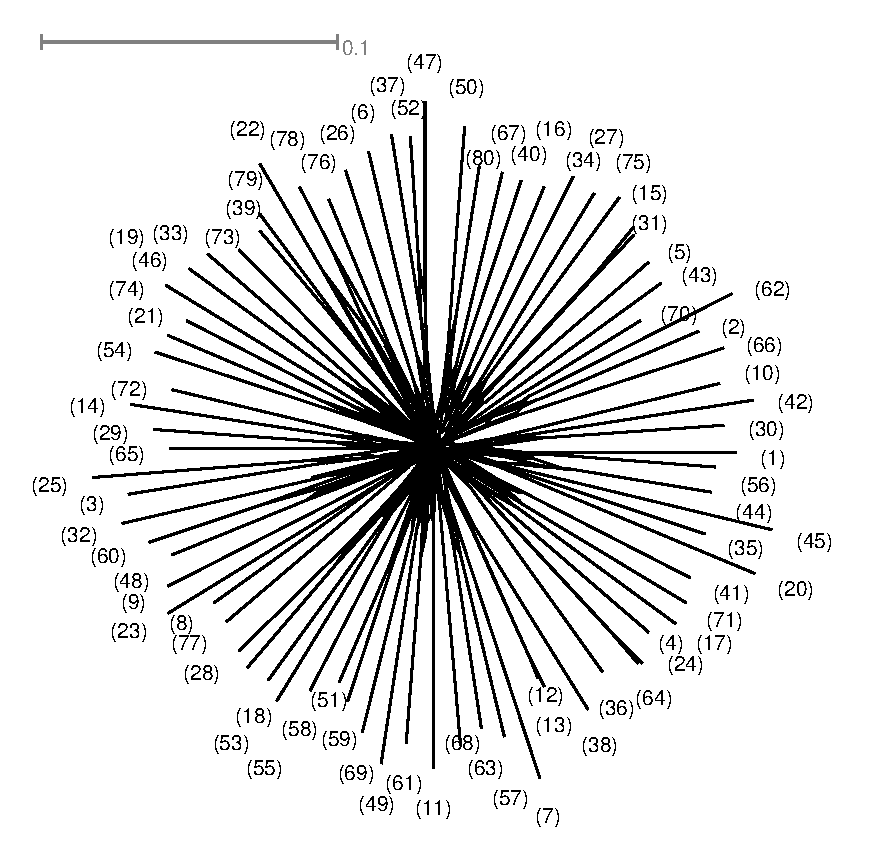
\includegraphics[width=0.5\textwidth]{Figures/Fcylindrus/Theta0_66Net}
}
\subfigure[$\theta = 0.066$]{
\includegraphics[width=0.5\textwidth]{Figures/Fcylindrus/Theta0_066Net}
}
\subfigure[$\theta = 0.0066$]{
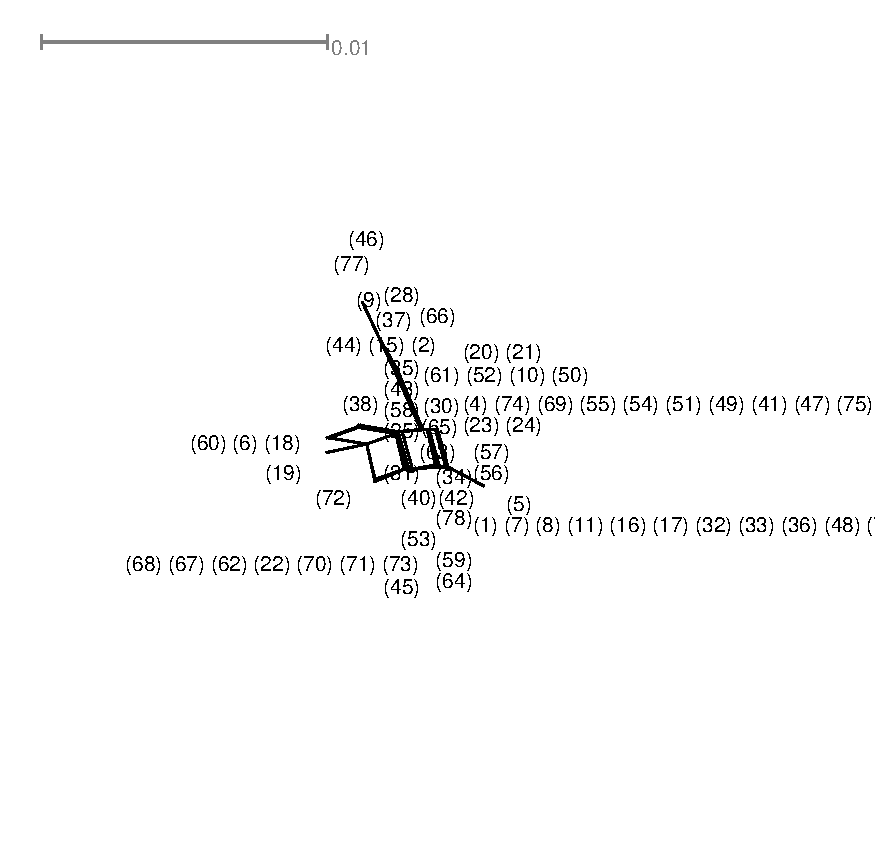
\includegraphics[width=0.5\textwidth]{Figures/Fcylindrus/Theta0_0066Net}
}
\caption{Networks computed from simulations with three different values of $\theta$.
Larger values of $\theta$ result in longer outer branches of networks.\label{fig:blnets}}
\end{figure}

Figure \ref{fig:blnets} presents this relationship qualitatively with the networks produced by Splitstree.
From figures \ref{fig:relgraphs} and \ref{fig:blnets} it can be seen that the networks best matching the real sequence networks (figure \ref{fig:realnets}) in terms of branch lengths, are those produced by simulations where $\theta = 0.066$, which is close to the value which LAMARC has estimated. 

Panel b of figure \ref{fig:relgraphs} demonstrates the effect of varying the recombination rate relative to the mutation rate in population genetic simulations, on the sequences and networks produced: The number of splits in networks is positively related to the recombination rate, relative to the mutation rate. This relationship is shown qualitatively in the networks drawn in figure \ref{fig:splitnets}.

\begin{figure}
\begin{center}
\subfigure[$R/\mu=1$]{
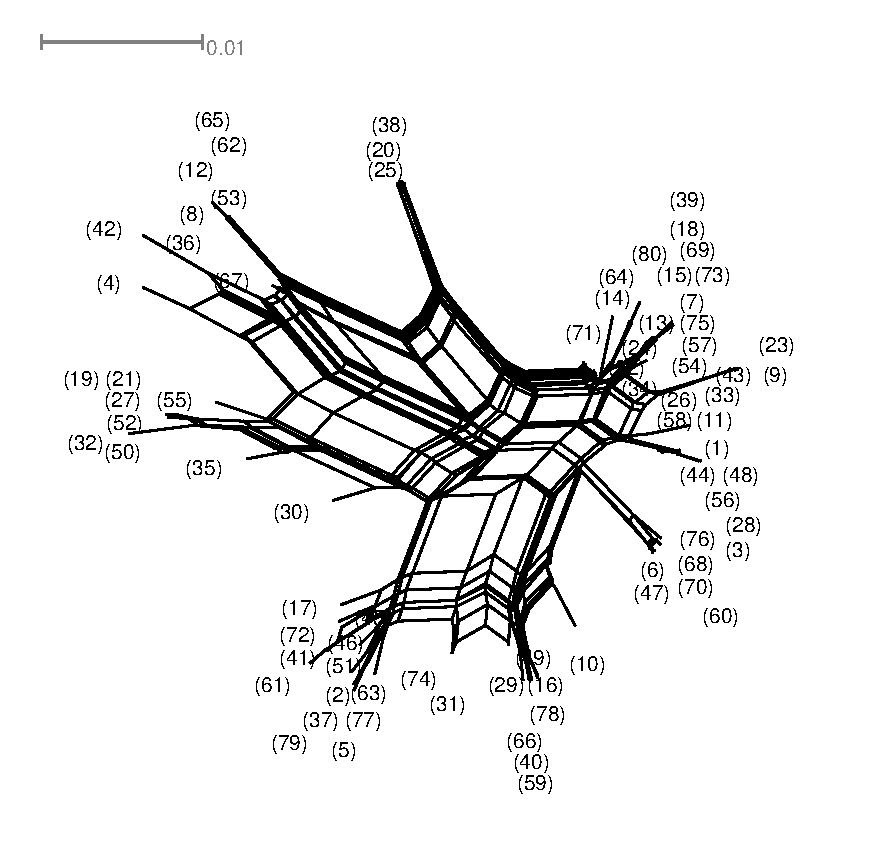
\includegraphics[width=0.5\textwidth]{Figures/Fcylindrus/rmuNet}
}
\subfigure[$R/\mu=5$]{
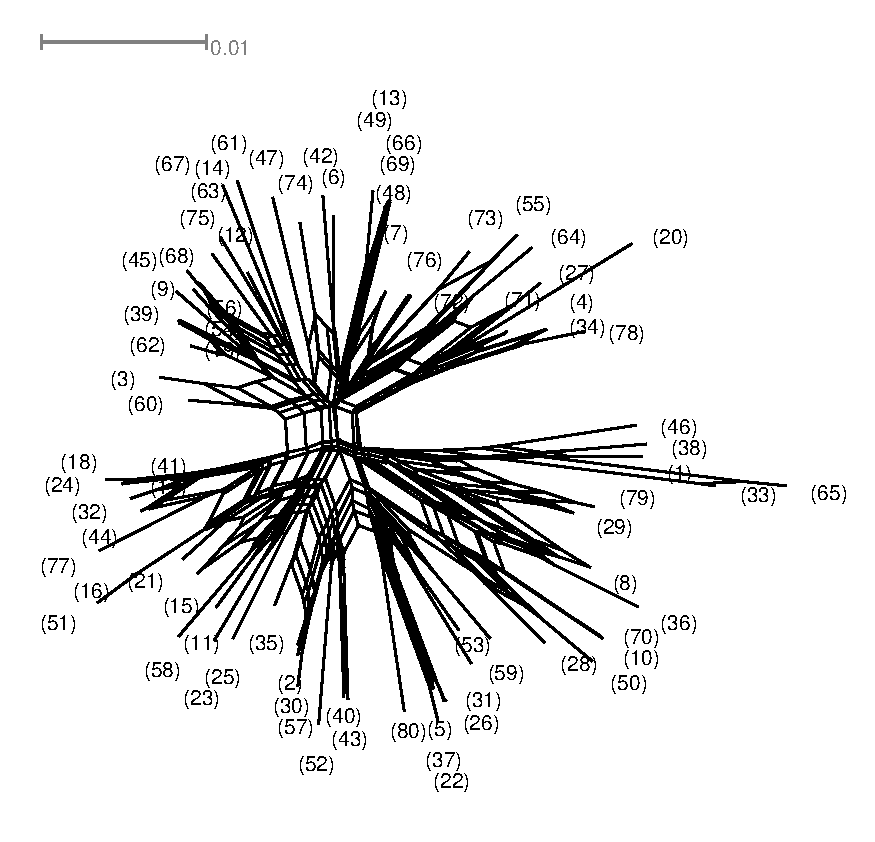
\includegraphics[width=0.5\textwidth]{Figures/Fcylindrus/rmu5Net}
}
\subfigure[$R/\mu=10$]{
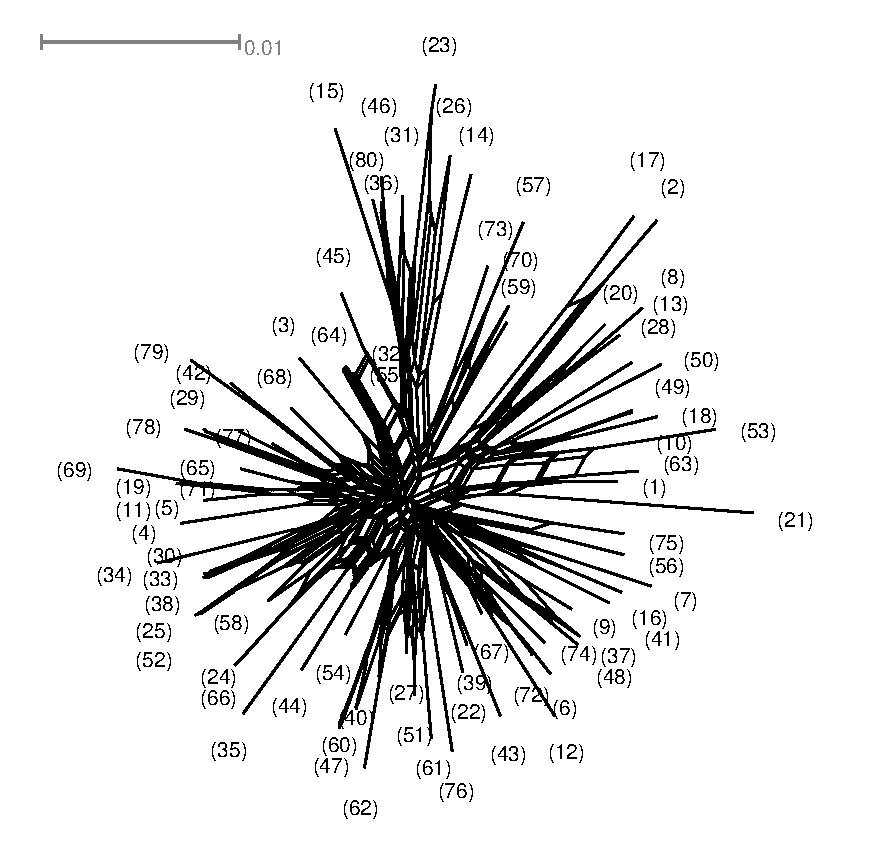
\includegraphics[width=0.5\textwidth]{Figures/Fcylindrus/rmu10Net}
}
\caption{Networks computed from simulations with three different levels of recombination, relative to the mutation rate $\mu$.
Larger values of $R$ result in more splits in networks.\label{fig:splitnets}}
\end{center}
\end{figure}





\section{Discussion}

The phylogenetic networks resulting from population genetic simulations support several assumptions we had about how recombination, and population mutation rate ($\theta$) may be inferred from phylogenetic networks.
Specifically, (1) the levels of Theta affect the average branch lengths of the networks, and (2) the extent of recombination affects the number of splits in phylogenetic networks.
These two assumptions are not controversial: a higher population mutation rate leads to more mutations in a population the same amount of time, and thus would lead to longer branches in any phylogeny or network computed for sequences sampled from the population \parencite{Frankham1996,Hein2004,Wakeley2008}.
Phylogenetic Split Networks \parencite{Huson1998} were conceived of as a way to detect and represent reticulate evolution.
Wherever there is a non-tree like structure or “loops”, recombination may be inferred.
The networks resulting from the simulations confirm these assumptions, and so give confidence in any inferences made about the population and evolution of \textit{F. cylindrus} from the networks of the ABC Iron Transporter sequences, and the Large Ribosomal Subunit Sequences.

Secondly, from comparisons between the networks of the ABC Iron Transporter sequences, Large Ribosomal Subunit Sequences, and simulated networks, it was concluded that LAMARC \parencite{Kuhner2006a} estimate of $\Theta$ was a reasonable estimate for the population of \textit{F. cylindrus}.
It was also concluded that these networks provide evidence of recombination for the sequences of the ABC Iron Transporter, and in the sequences of the Large Ribosomal Subunit.
Evidence of recombination does not have to mean that an organism is reproducing sexually, meiotic recombination is associated with sexual reproduction, but mitotic recombination could also explain the recombination signal detected in these sequences.
However, whilst mitotic or meiotic recombination may explain the recombination signal in the sequences, it was concluded that ancient asexuality is not a likely explanation, because of the lack of similarity of the ABC Iron Transporter, and the Large Ribosomal Subunit networks, to the networks generated by simulations of ancient asexual evolution.


\subsection{Sex and the diatom reproductive cycle}

Even though sexual reproduction has not been observed in the lab cultures of \textit{F. cylindrus}, this diatom does not appear to be an ancient asexual.
This might not be surprising given what is already known about Diatom biology and sexual reproduction.
The typical cell cycle of Diatoms is diplontic i.e. the vegetative cells are diploid, and the haploid gametes are short lived \parencite{Chepurnov2004}.

The Diatom life cycle features two key phases which may be summarized by the following:

The first phase is a long vegetative phase; this phase can last for months or years. During this phase, vegetative cells divide by mitosis, gradually becoming smaller. 
The cell size decrease during the vegetative phase of the diatom life cycle is due to the shape and structure of Diatom cell walls and the division pattern of the Diatoms. 
The cell wall is made of sillicated components, which together are termed the frustule. The frustule is made of two overlapping halves or thecae \parencite{Chepurnov2004,Davidovich1998,Poulickova2008}.
These thecae are not the same size, the larger of the two thecae is called the epitheca, and the smaller of the two is called the hypotheca.
When mitosis occurs, cytokinesis splits the diatom where the two thecae overlap.
The two resulting daughter cells inherit one of the parent cell’s two thecae as its own epitheca, and they grow their own hypotheca \parencite{Chepurnov2004}.
Since one of the daughter cells inherits a hypotheca as it epitheca, it will be smaller in size to its parent cell.
Thus the average cell size of a population of diatoms decreases as mitotic cell division occurs.

The second phase is shorter, and includes sexual reproduction and the production of new vegetative cells, restoring the cell size \parencite{Chepurnov2004}.
Production of gametes during the sexual reproduction phase has been demonstrated to occur by classical meiosis in many Diatom species.
Diatoms restore their cell size through the production of auxospores, which result from sexual reproduction \parencite{Davidovich1998}.
During auxosporulation, recombination and cell size restitution occurs: gametes fuse to form the auxospore, which expands and a new cell is produced within.
The cell walls of the gamete producing cells are lost, and so the auxospore must then form the shape of the vegetative cells de novo \parencite{Chepurnov2004}.
If a population of Diatom cells did not undergo sexual reproduction to produce the auxospores to restore their cell size, the population would gradually decrease in cell size until they become critically small.
At this point the population would die, and this has been observed in experimental cultures.
Diatom cells can only become sexualized when they are sufficiently small, but they may also not be able to become sexualized if they become too small or hit the critical cell size before they die \parencite{Chepurnov2004,Davidovich1998,Poulickova2008}.
The maximum size of initial diatom cells, the maximum and minimum sizes of cells capable of sexual reproduction, and the minimum size before death are strict for each diatom species and are termed cardinal points \parencite{Chepurnov2004}.

However, despite the role of sex in the restoration of cell size in diatoms, it is not always necessary for cell size restoration.
For some diatom species, asexual auxosporulation is a possibility, presumably it is some secondary modification of a developmental pathway that was sexual, and some species do not even undergo auxosporulation and exist as entirely as asexual populations, and their cell size is restored by vegetative cell enlargement \parencite{Chepurnov2004,Gallagher1983,Nagai1995,Sabbe2004,werner1977biology}.
Species such as \textit{Caloneis amphisbaena} and \textit{Sellaphora pupula} "lanceolate" have been found to exist in populations of a very limited range of cell size, and this cell size has remained unchanged after many generations of observation \parencite{Mann1989,Mann2004}.

Therefore, whilst sex is a common feature of the diatom life cycle, and is important for cell size restoration in many species, it is not unreasonable to suggest the hypothesis that a diatom like \textit{F. cylindrus} could have evolved asexually for a long period of time.
However, the network reconstructions and evidence of recombination demonstrated by this study cast doubt on that hypothesis as an explanation for the diverged alleles.


\subsubsection{Allelic Divergence in diatoms may be explained by population size}

If the “ancient asexuality hypothesis” is rejected as the explanation of the diverged alleles in \textit{F. cylindrus}, then an alternative explanation of how this diatom evolved diverged and functionally differentiated alleles is desired.
These alleles show signatures of positive selection, and they are differentially expressed.
The question is; assuming sexual reproduction and recombination, why does recombination not homogenize the sequence variation between two alleles over time? 

An alternative hypothesis explaining the adaptive evolution of \textit{F. cylindrus} is a large population size, which would lead to bigger coalescence times between maternal and paternal loci.
In combination with a low recombination rate, this would result in independent adaptive evolution and divergence of the different haplotypes.
This is intuitive if one considers a coalescent process back through time of an idealized population, because the coalescent relates genetic diversity to demographic history.
In such a process, the probability that any two lineages extant at time $t$, coalesce in the previous generation $t – 1$, is the probability that they share a parental DNA sequence.
For a diploid population there are $2N_e$ alleles in every generation, assuming a constant population size \parencite{Hein2004}.
Assuming random mating and neutral evolution, the probability any two alleles coalesce in the previous generation (i.e. they share the same parental sequence) is $1 / (2N_e)$.
Therefore, the probability those two alleles do not coalesce, is $1 – (1/(2N_e))$.
These probabilities are dependent on the size of the population in question \parencite{Wakeley2008}.
Larger populations, result in a smaller probability that two alleles coalesce in the previous generation, and a greater probability that they do not.
With each successive previous generation, the probability of coalescence is geometrically distributed \parencite{Hein2004,Wakeley2008}.
This means that it is the product of coalescence at the generation of interest and the probability of non-coalescence at the preceding generations i.e.
\begin{equation}
P_c(t)=\bigg(1-\frac{1}{2N_e}\bigg)^{t-1}\bigg(\frac{1}{2N_e}\bigg)
\end{equation}
From this equation, it can be seen that with larger populations, the probability that two alleles coalesce further back in time is greater i.e. the expected coalescence time between two alleles is larger, therefore alleles are expected to be more diverged.

This explanation is consistent with the estimation of a $\Theta$ of 0.066 by the LAMARC \parencite{Kuhner2006a} analysis, which is also supported by the simulations.
The population mutation rate $\Theta$, is proportional to the product of the mutation rate and the effective population size and so the value predicted by LAMARC could be the result of a very large population.
Furthermore, prior research has been performed to estimate the abundance of \textit{F. cylindrus} in water columns around the Antarctic \parencite{Kang1992}.
During the summer, numbers of $7.9 \times 10^{10}$ cells $^{m-2}$ were observed, and during the winter, numbers of $1.1 \times 10^8$ cells $^{m-2}$ were observed.
Marginal ice zones are known to be sites with much dynamic activity such as jets, eddies, currents, melting, freezing, and upwelling \parencite{Kang1992}.
They are also known to be sites of increased phytoplankton biomass and primary productivity, due to their light levels, ice-distribution, and vertical stability.

Therefore, the hypothesis that a large population size explains the levels of diversity is consistent with both population genetic (coalescent) theory, results of this study, as well as the findings of other research.
It is also attractive, because of its simplicity.
It is much more plausible that a phytoplankton species has very large populations; than it is that the species had abandoned sex as a reproductive strategy:
Sex is a common aspect of the diatom life cycle and is often essential for cell size restoration and population survival.
Furthermore, as was explored in the Introduction, there is a substantial body of theory explaining why sexual reproduction evolved two become a widespread reproductive strategy, and is advantageous, despite the apparent costs.


\subsubsection{Study limitations and subsequent FALCON assembly}
However, this study has some limitations which should be acknowledged when considering these results.
First, whilst evidence of recombination in the form of the splits networks and the presence of incompatible sites is obtained from these sequences, it was not possible to examine any larger recombination events or blocks as was possible for \textit{Albugo candida} in chapter \ref{chap:Acandida}.
Indeed, the number of informative sites was too small for the HybridCheck software (which was implemented to analyse large contigs) to effectively run.
Secondly, the analyses were only performed on two genes.
Whilst it was concluded that the two genes were representative of the larger set of diverged alleles (figure \ref{fig:FC_Res_1}), we do not know if the PCR primers amplified only maternal and paternal alleles of those genes or if some of the sequences amplified also represent paralogues.

The question of whether the diverged alleles observed in the assembly were truly diverged alleles was resolved for the assembly described in the introduction experimentally.
Single haplotyped fosmids were Sanger sequenced by collaborators, providing contiguity information and they were compared with the assembled genomic scaffolds, and an annotated protein set from the diverged regions in the genome.
Data from these comparisons revealed a clear separation between allelic pairs and gene duplications based on 100\% identity to the haplotyped Sanger sequenced fosmids.
Additionally, the nucleotide similarity of the diverged alleles (mean = $97.01 \pm 0.03\%$) is significantly (p-value $< 10^{-09}$) higher than for gene duplicates (mean = $84.07 \pm 0.36\%$). 
Therefore, whilst it may be that some uncollapsed regions of the assembly could be duplicates, there is high confidence that the allelic pairs identified are indeed diverged alleles and not duplicates.

Since this work has been completed, an assembly has been completed using PacBio long read sequencing technology, which has also supported that true diverged alleles have been identified and that they are not duplicated sequences (although duplicated sequences are indeed present in the genome). 
The sequencing work and library preparation was completed by the platforms and pipelines team.
A 20kb fragment length library was constructed, and a 4kb insert size library was also created. 
Both libraries were sequences using the PacBio RS2 instrument, using SMRT cells with the c4P6 chemistry.
The 20kb fragment length library yielded 1.37Gb of data, and the 4kb insert size library yielded 3.85Gb of data.
The final N50 of read length varied between 8215 to 8898bp for the 20kb fragment length library, and the N50 ranged from from 2558 to 2680bp for the 4kb insert size library.

Assembly was completed by collaborator Pirita Paajanen, who combined the data from the SMRT cells and filtered the shortest reads, yielding 3.8Gb of data which gave 63x coverage.
Assembly was completed using the diploid aware PacBio assembler, Falcon 0.3.0.
The output of the Falcon assembler was divided into two parts.
The haploid assembly resulted in primary contigs from which a genome size of 59.7Mb was deduced. 
However, the assembler also produced alternate contigs which were the result of the assembler being unable to decide between two possible routes through the genome graph the genome.
Such 'bubbles' in the genome graph represent diverged haplotypes, containing diverged alleles.

The haplotype divergence differed between chromosomes: The longest chromosome 000000F had only one alternate contig with a length of 6047bp.
In contrast, contig 000002F was 1246645bp long and had 14 associated alternative contigs, of a total sequence length of 633764bp.
For each of the 14 alternative contigs of chromosome 000002F, I extracted and aligned the two haplotype sequences using the pairwise alignment algorithm available in the Bio.jl software package (https://biojulia.github.io/Bio.jl), using an EDNA scoring matrix.
Once aligned, a non-overlapping sliding window was moved across the sequences, and the p-distance between the sequences within each window was calculated. For each computation, the width of the sliding window was set as 1\% of the width of the pairwise alignment in (bp).
The results of this analysis are included as extra information in the appendix, figure \ref{fig:falconwindows}.
The figure demonstrates different levels of divergence across the diverged haplotype pairs, including the appearance of indels between some haplotype pairs.
Further work will show how the sequences of allelic pairs align to the FALCON assembly, revealing which pairs align to different haplotypes of a FALCON 'bubble' (true allelic pairs), and which pairs align to the same haplotype of a FALCON 'bubble' (potentially gene duplicates).

At the time of writing, multiple population samples of \textit{F. cylindrus} are not available, and so analyses presented here used sequences from cultures, and so further population genetic analyses should be conducted in the future as more data becomes available, for example to assess the population structure of \textit{F. cylindrus} and investigate if gene flow is occurring between subpopulations of \textit{F. cylindrus}.

The fact that the genome assembly contains some duplicates, and that some of the allelic pairs analysed in this study may be found to be duplicates is not problematic for the hypothesis that this Diatom species has adapted through alleleic divergence, as it may be argued allelic divergence could lead to gene duplication and the conditions for the divergence of alleles and the divergence of duplicates overlap: 
When diverged alleles are maintained in a population due to heterozygote advantage, duplications may rapidly spread through the population, causing an individual to act as a genetic heterozygote yet still breed true.
\cite{Proulx2006} argued that genetic redundancy is the mechanism usually cited as allowing duplicate genes to diverge, but redundancy is present in a diploid before duplication: Dominance creates the same kind of redundancy duplicates have, but for alleles of single copy genes.
Therefore mode of inheritance is the thing then which most distinguishes duplicates from single copy genes: Segregation prevents the fixed inheritance of alternative allelic variants at a single locus \parencite{Proulx2006}.
In other words, heterozygotes at one locus are broken up by segregation during sexual reproduction, whereas duplicate loci in an individual can carry copies of alternate alleles at different loci.
Their results show that fitness relationships that allow divergent alleles to evolve at one locus overlap significantly with those that allow the divergence of previously duplicated genes at two different loci \parencite{Proulx2006}.


\subsubsection{Conclusion}

The genome of the polar diatom \textit{Fragilariopsis cylindrus} contains diverged alleles that are differentially expressed in different environmental conditions.
Evidence of recombination was found which contradicts the ancient asexuality hypothesis explaining how these diverged alleles may have evolved.
An alternative, competing hypothesis is proposed, supported by the evidence presented, that a large population size has allowed diversifying selection to differentiate the alleles of genes despite the homogenizing effect of recombination.
Additional population samples, and analysis of larger contigs made possible by improved genome assembly for recombination, will help answer the question of how \textit{F. cylindrus} has evolved this remarkable strategy to cope with varying environmental conditions.




\setcounter{chapter}{4}
\chapter{General Conclusion}

\subsection{Summary and Conclusions}

In this thesis, work focused on how recombination facilitates the adaptive evolution of a plant pathogen and a polar marine diatom.
Both of these organisms were of evolutionary interest due to aspects of their lifestyles and/or physiology:
The plant pathogen \textit{Albugo candida} was of interest because whilst it was an obligate biotroph, it has a very large host range, and the diatom \textit{Fragilariopsis cylindrus} was of interest because the genome sequencing project and differential expression experiments revealed genes with diverged alleles that were differentially expressed in different environmental conditions.

Recombination is important for the formation of novel genotypes, haplotypes and alleles, therefore is plays a key role in adaptive evolution \parencite{Grauer2000}.
Recombination separates deleterious mutations from their genomic background, in combination with purifying selection this reduces the mutational load \parencite{Lynch1990a}.
Recombination also brings beneficial mutations from separate lineages into one individual or lineage.
However, recombination also plays a fundamental role in the repair of damaged DNA, when homologous recombination replaces a damaged DNA strand with its intact counterpart, and it was likely this function of recombination that was important in early prokaryotic life and evolution \parencite{Cavalier-Smith2002}.
With respect to adaptive evolution, however, the principal consequence of recombination is that it generates novel combinations of nucleotides, which in turns allows for selection to act a much finer scale, i.e. at the level of nucleotides rather than the entire genome.

The potential of recombination to generate novel allelic combinations is important for host and pathogens which are engaged in an evolutionary arms race to adapt and counter adapt to each others molecular mechanisms of pathogenicity or immunity.
The red queen hypothesis explains the advantage of sexual reproduction in such terms.
The variability generated by sexual reproduction (and meiotic recombination) results in genetically unique offspring, which permits a faster response to selection \parencite{Paterson2010}.
As a result sexually reproducing species are able to improve their genotype in changing conditions. 
Co-evolutionary interactions between host and parasite select for sexual reproduction in hosts in order to reduce the risk of infection.
Oscillations in genotype frequencies are observed between parasites and hosts in an antagonistic co-evolutionary way without necessitating changes to the phenotype, and in host-parasite co-evolution systems with multiple hosts, Red Queen dynamics may affect which host and parasite types become common (or rare) \parencite{Charlesworth2010}.

It was hypothesized that the \textit{Albugo candida} species was composed of several host-specialised races, each locked in an evolutionary arms race with their specific host.
Such a race with a specific host would lead to further divergence and possibly speciation of the races.
However, \textit{Albugo} is known to be able to suppress non-host resistance.
Infections of \textit{Albugo sp.} could suppress the runaway cell death phenotypes of plants, allowing formerly avirulent strains of downy mildew to infect \parencite{Cooper2008}.
Assuming that this ability extended to other non-host species, \textit{Albugo} may be modeled as a 'microbial hub': taxa that are integral and highly connected to the network of a hosts microbial community.
Such hubs may affect community compositions through microbe-microbe interactions or, as seems to be the case with \textit{Albugo}, suppression of host defense responses \parencite{Agler2016}.
Therefore, non-host immune suppression would enable host-specific races of \textit{Albugo candida} to overcome the ever increasing barrier to gene flow that specialisation imposes, and sexual reproduction between races, followed by introgression by back-crossing, would permit the generation of a range of novel genotypes.
Consequently the species could evolve its wide host range.

To assess this hypothesis it was necessary to scan the genome of \textit{Albugo candida} isolates to identify recombinant regions.
Furthermore, to distinguish such regions as recombinant and not the result of incomplete lineage sorting due to rapid divergence, the regions identified needed to be tested for significance and the coalescence times estimated.

Scans of the genomes for recombination revealed a highly recombined mosaic genome, and therefore a rapid coalescence estimation method for all of the recombination blocks was desired, in addition to a method of plotting which effectively demonstrated the high degree of mosaic-ism in the \textit{A. candida} genome.
Therefore, rapid detection and dating of recombination blocks was implemented, and the software package HybridCheck was created  and tested using simulated data as in chapter \ref{chap:HC}.
HybridCheck was also tested for consistency with RDP analyses of \textit{A. candida}, which identified recombination, and BEAST estimates of coalescence times for a subset of the identified recombination regions (chapter \ref{chap:Acandida}).
The evidence presented in chapter \ref{chap:Acandida} confirmed the model of \textit{Albugo candida evolution}:
Isolation, divergence and specialisation of races generates repertoires of effectors for a specific race.
Those adapted repertoires are then brought together when two races hybridize.
The result if the generation of novel repertoires of novel combinations of these effectors.
Specific avirulence effectors that trigger host immunity may be lost through segregation and through loss of heterozygosity \parencite{Lamour2012PathogenCapsici,McMullan2015a}.
Hybrids, with new combinations of effectors, and having lost effectors which impeded their colonisation of other hosts previously, may expand their geographical range and population size clonally.
Some of these hybrids may be able to colonise new hosts, expanding the host range.

The genome assembly project of \textit{F. cylindrus} revealed that the genome contained 21,066 predicted protein-encoding genes, 6,071 genes were represented by diverged alleles, and each pair of diverged alleles had both coding and non-coding regions, and were up to 6\% polymorphic in the non-coding regions.
Furthermore, differential expression experiments and RNA-Sequencing suggested that 40\% of
the non-collapsed, diverged allelic pairs showed a 4 fold unequal bi-allelic
expression \parencite{Mock2017}.

Alleles showing the strong unequal bi-allelic expression were found to have an
elevated rate of non-synonymous mutations, which suggests significant positive
/ adaptive selection and evolution of these allelic pairs \parencite{Mock2017}.
It was concluded therefore, that positive selection has been a driving force in
the evolution of these diverged alleles and hence the adaptation of this diatom to the
environmental conditions it faces.

An evolutionary explanation was hypothesized: The alleles of an allelic pair could diverge as a result of positive selection because there was a long history of asexual reproduction in the organism, and hence an absence of recombination acting as a homogenizing force between alleles.

However, results from recombination detection analysis, and phylogenetic network construction of PCR amplified sequences from DNA extracted from \textit{F. cylindrus} cultures conflicted with results of the same analyses performed with DNA sequences obtained by population genetics individual based simulations of ancient asexuality.
Indeed the results for \textit{F. cylindrus} were more consistent with those of simulations of a scenarios of sexual reproduction, and a large $\Theta$ value.
This result suggests an alternative competing hypothesis, that very large effective population sizes could have led to the divergence of the alleles in each allelic pair as a result of positive selection, in the face of the homogenizing influence of recombination through sexual reproduction.


\subsection{Impact and potential future directions}

\subsubsection{\textit{Albugo candida}}

A paper describing the extent of the introgression identified within the \textit{A. candida} genome was published in eLife \parencite{McMullan2015a}.
According to Google Scholar, the study has been cited 11 times at time of writing.
Citations include reviews of the role of hybridisation and introgression in the adaptive evolution and emergence of new fungal and filamentous plant pathogen strains \parencite{Depotter2016,Dong2015,Stukenbrock2016}, research demonstrating the role of recombination in the evolution of the Rp1 resistance genes in grasses \parencite{Jouet2015}, and a study presenting evidence that for \textit{Coleosporium ipomoeae}, any genotypes can infect multiple hosts from non-local communities, but only are highly host specific when tested on hosts from local communities, calling into question theoretical results of single-pathogen single-host studies which suggest that selection favours genotypes with a broad host range \parencite{Chappell2016}.
Following the 2015 eLife paper, \cite{Belhaj2015} published a more extreme example of the ability of \textit{Albugo spp.} to suppress the host immune system.
They found that \textit{Phytophthora infestans}, which is typically a potato and tomato specialist pathogen, was capable of infecting the plant model organism \textit{Arabidopsis thaliana} when \textit{Albugo laibachii} has also colonized the plant.
The nature of the \textit{P. infestans} infection was similar to that of an \textit{Albugo laibachii} infection: Transcription profiling of \textit{P. infestans} infections revealed a significant overlap between the sets of secreted proteins of \textit{P. infestans} during infection of \textit{Arabidopsis thaliana} and during infections of potato.
This suggests there is similar gene expression dynamics on the two species, and it raises the question.
Is gene flow between two different Oomycete species possible? And could this contribute to adaptive evolution of these pathogens.

It is well established that \textit{Albugo} suppresses hon-host immunity in hosts it infects, and as a result of work presented in this thesis it was concluded that this lowers barriers to gene flow and permits introgression, facilitating the generation of novel pathogen haplotypes and enabling \textit{Albugo candida} to evolve a wide host range.
However, this model of \textit{Albugo candida} evolution raised a conceptual problem: 
This phenomenon  appears to extend to other pathogen species that were not \textit{Albugo spp.} \parencite{Belhaj2015}, and therefore \textit{Albugo spp.} may act as a microbial hub as previously noted.
If this is the case, how is it that \textit{Albugo spp.} (obligate biotrophs with a vital dependence on the host) can compete in this limited niche, whilst at the same time enable non-host colonization for other pathogen species who are then presumably competitors for the same resource.
An answer to this problem was provided by a paper from \cite{Ruhe2016}.
Shotgun proteomics was completed of the apoplastic fluid of samples of lab-grown \textit{Arabidopsis thaliana} that were infected with \textit{Albugo spp.}, and samples which were uninfected.
Work was repeated for wild-grown \textit{Arabidopsis thaliana} and they found that whilst both lab-grown and wild-grown \textit{Arabidopsis thaliana} supported extensive \textit{Albugo} colonization \parencite{Ruhe2016}.
However, no or low levels of defense-related proteins were detected in lab samples, but regardless of \textit{Albugo spp.} infection status, wild plants showed a broad spectrum of defense-related proteins at high abundances and lab-grown plants did not.
These results suggest that \textit{Albugo spp.} do not strongly affect immune responses and leave distinct branches of the immune signaling network intact \parencite{Ruhe2016}.
This suggests that the pathogens of the \textit{Albugo} genus, including \textit{Albugo candida} in the wild are fine tuned to avoid triggering strong host defense reactions, but also to avoid a broad-spectrum host defense suppression, thus allowing them to avoid competition from other species growing in the same niche \parencite{Ruhe2016}.
Since races of \textit{Albugo candida} are members of the same species, they may still colonize the same host plant at the same time, allowing introgression to occur (explaining the introgression signal observed), but other more distantly related competing pathogens may be excluded by this precise host immunity manipulation observed by \cite{Ruhe2016}, and so may not get to compete with \textit{Albugo spp.}.
However this experiment only examined \textit{Arabidopsis thaliana} as a host, and crops grown in monoculture are often uniform and subject to artificially maintained conditions and treatments, and this may be considered analogous to plants grown in laboratory conditions.
So it is uncertain whether in monoculture environments \textit{Albugo spp.} manipulate their host immune systems subtlety and precisely, thus avoiding colonization of competition, or whether as with lab-grown \textit{Arabidopsis thaliana} they do significantly affect the secretome of the host, allowing competitors to colonize.

In the future, additional study of more strains and population samples of \textit{Albugo candida} is desirable, since the study presented in this thesis only examined the genomes of three 'races', and more samples might increase the number of \textit{Albugo candida} races we can analyse.
Future potential work also includes disentangling the true branching order of \textit{Albugo candida} races, and improving the detection and dating methods used to analyse \textit{Albugo candida} genomes (see below).


\subsubsection{HybridCheck}

The HybridCheck software package was initially created out of a need specific to the \textit{A. candida} project in chapter \ref{chap:Acandida}.
Following the \textit{A. candida} project, the HybridCheck software was published in a short software note in Molecular Ecology Resources \parencite{Ward2016}, and other groups across the Norwich Research Park became interested in using it with their own study systems.

In particular, researchers at Norwich Medical School working on \textit{Cryptosporidium} used HybridCheck to perform chronological assessment of recombination events identified in the genomes of  
three trains of \textit{C. parvum} (IIaA15G2R1, IIcA5G3j, IIcA5G3a), and a single \textit{C. hominis} (IbA10G2) GP60 sub-type strain \parencite{Nader}.
They found 104 unique recombination events, and a skewed distribution of recombination events across chromosomes.
More recombination events were identified on chromosome 6, and a greater number of events was observed for \textit{C. parvum anthroponosum} sub-type IIcA5G3a than for any other strain.
More than 90\% of all recombination events occurred proximal to loci suspected to drive virulence or play a major role in host-parasite interactions in human cryptosporidiosis.
Therefore it appears that in this pathogen too, recombination is an important force, generating novel gene combinations and driving the adaptive evolution of a pathogen to its host \parencite{Nader}.
The estimated divergence dates calculated in their study provide the first chronological description for genetic introgression between human-infective \textit{Cryptosporidium spp.}.
HybridCheck analyses revealed a chromosome-wide consensus that places a majority of introgression events between zoonotic (IIaA15G2R1 and IIcA5G3j) and anthroponotic (IIcA5G3a) \textit{C. parvum} sub-type strains at approximately 10-15 thousand generations ago, while genetic introgression (or recombination) between the two more closely related zoonotic strains appears to be more recent (between approximately 3 to 5 thousand generations ago) \parencite{Nader}.

Based on infectivity studies in healthy adult volunteers, the average generation time within a host is 14.8 hours, and assuming a steady rate of transmission within host populations, they derived a minimum estimate of the recombination events of around 5.9 (zoonotic vs. zoonotic \textit{C. parvum}), 17.6 (zoonotic vs. anthroponotic \textit{C. parvum}), and 176.7 (\textit{C. hominis} vs. \textit{C. parvum}) years ago \parencite{Nader}.
In other words, they estimate that the evolutionary split between the two primary human-infective species appears to have occurred at the turn of the second industrial revolution, around 1840 \parencite{Nader}.

Whilst this result is putative and needs validation with other dating methods before publication submission, it is a clear demonstration of the utility of HybridCheck for researchers in estimating coalescence times rapidly, across many recombination affected genomic regions.

Future directions for work involving HybridCheck include its continued use in other organisms.
For example HybridCheck is already being used to generate preliminary results for population genomic data for mice (\textit{Mus spp.}), being generated at the Earlham Institute, with the aim of confirming hypotheses of genetic isolation between species, and identifying potential introgressions between populations.
Future work involving HybridCheck may also involve programmatic work.
Bioinformatics methods and the detection of introgression is an active area of research, and more algorithms and methods will likely be created in the future.
Therefore, HybridCheck would have greater utility as a provider of different methods for the detection and dating of recombinant and introgressed regions, that are able to work on multiple different data sources or formats.
As a programming problem, such software code might be best implemented, using multiple dispatch, to make it more easily maintained, and more easily used.
Multiple dispatch is a feature of some programming languages in which a function (sometimes called a  method) can be dynamically dispatched based on the type of more than one of its arguments.
This thesis author has already co-founded, develops, and maintains a new bioinformatics infrastructure and community called BioJulia, based around a modern new programming language for scientists and technical programmers, called Julia.
The language is high-level, implements a flexible type and multiple dispatch system, and can achieve speeds matching those of compiled software written in the C language, with less lines of code.
These features make it ideal for the kind of rapid and flexible development that Bioinformaticians often do, and should development of HybridCheck continue towards this goal, the framework already has many high performance code modules and features that a BioJulia port of HybridCheck could take advantage of.

In the near future, approaches to recombination detection may also change.
Currently, HybridCheck and other methods typically analyze DNA or protein sequences and identify regions that are phylogenetically incongruent i.e. where computed phylogenetic topologies change or there is a change-point in computed genetic distances.
After the identification of these regions, it may be assumed they are recombination, or incomplete lineage sorting, and subsequent analyses, such as the dating method in HybridCheck, may be employed to try to distinguish whether the cause is recombination or incomplete lineage sorting.
The cause may also be assumed based on rates of speciation or population size; incomplete lineage sorting is more likely when either of the two are high.
However, as described in chapter \ref{chap:HC}, there are problems with this approach which leave room for future improvement.

For example, recombination blocks can become fragmented by accumulation of subsequent mutations following the recombination event.
Consequently, older recombination blocks tend to be smaller, when they are actually larger.
Thus, not all mutations are accounted for, resulting in an underestimate of the divergence time particularly for old recombination events/regions of incomplete lineage sorting.

Furthermore, some methods of resolving introgression from incomplete lineage sorting require knowledge of branching orders, and sometimes these are unknown, and sometimes this is even because of the influence of introgression or incomplete lineage sorting.
To solve this issue for the malaria parasite, \cite{Neafsey2014} obtained the correct species branching order of the \textit{An. gambiae} complex and two Pyretophorus out-group species.
To do this in the face of introgression and incomplete lineage sorting they used 50kb non-overlapping windows across a genome alignment and computed phylogeneies for each window.
At least 85 tree topologies were observed.
When these were sorted according to chromosome arm and their relative frequency, the most commonly observed topology for the X chromosome was highly discordant with the most commonly observed topology for the autosomes.
They then grouped these phylogenetic toplogies, into three distinct topology categories based on the relative phylogenetic positions of two species: \textit{An. arabiensis} and \textit{An. quadriannulatus}, and they observed the topology category most commonly observed on the X chromosome, was not the same as for the autosomes. 
Dating the internal nodes of phylogeneies for each topology category allowed them to distinguish which category of topology best represented the true branching order, and which represented topologies that were caused by introgression.
Given that almost all of the autosome was represented by a topology category that is affected by introgression and linkage disequilibrium, traditional phylogenetic methods for resolving a species level topology, which typically invoke some majority rule, would certainly have resulted in the incorrect answer.

The method utilized in their work will be of great benefit to researchers studying complicated genomes where introgression, and incomplete lineage sorting, are prevalent.
A likely future direction for the development of HybridCheck will be to take these methodological ideas and implement tools that make it trivial for researchers to decompose the gene trees computed across a genome, identify topological categories from those trees, and organize them, before analyzing the divergence times of the phylogenies in each topological category.
In the future HybridCheck should make it simple to perform such an analysis along with other methods such as Patterson's D, $f_d$, and tests to distinguish introgression from incomplete lineage sorting.
It should make it trivial to compile such multiple lines of evidence into a more complete picture of introgression, incomplete lineage sorting, and linkage, across genomes.


\subsubsection{\textit{F. cylindrus}}

The study of \textit{F. cylindrus} is in preparation to be submitted to the journal Nature this year.
As such it is not possible to describe the impact in terms of a number of citations, or who has cited it and why at this time.
However, as stated in discussion of chapter \ref{chap:diatom}, reviewer comments led to further sequencing with PacBio technology, which resulted in confirmation that we had obtained strong evidence of diverged alleles.
Furthermore, it is known that at time of writing, that unpublished data and correspondence from a colleague and co-author of the paper, Chris Bowler (perscom), that similar evidence of diverged alleles and differential expression has been found in another diatom species that his group study.
Therefore, it could be that the data presented in this thesis and in the paper, are the first evidence of a common phenomenon and mechanism of adaptation in this group of organisms.
Future work on this topic has already been described in the discussion of chapter \ref{chap:diatom}:
Imminent future work will show how the sequences of allelic pairs previously identified align to the new FALCON assembly.
This will reveal which pairs align to different haplotypes of a FALCON 'bubble' (true allelic pairs), and which pairs align to the same haplotype of a FALCON 'bubble' (potentially gene duplicates).
Currently, multiple population samples of \textit{F. cylindrus} are not available, and so analyses presented here used sequences from cultures, and so further population genetic analyses should be conducted in the future as more data becomes available, for example to assess the population structure of \textit{F. cylindrus} and investigate if gene flow is occurring between subpopulations of \textit{F. cylindrus}.

In conclusion, detecting and understanding how recombination is affecting the genomes is critical to understanding how species of interest evolve and adapt to dynamic environments, this thesis has demonstrated how recombination appears to have influenced the evolution and adaptation of two different eukaryotic micro-organisms.
Future work will expand on the bioinformatics methodological techniques implemented in this thesis, as more and more data becomes available for these two species.  





%=======================================================================
% Bibliography
%=======================================================================
\printbibliography

%=======================================================================
% Appendices
%=======================================================================
\begin{appendices}

\chapter{FALCON assembly haplotype divergence}
\begin{figure}
\includegraphics[scale=1.0]{Figures/Fcylindrus/Diatom_FALCON_1-100_panels}
\caption{Sequence similarity calculated with sliding windows across each haplotype 'bubble' in chromosome 000002F, from the \textit{F. cylindrus} FALCON genome assembly.
Regions of divergence and indels are apparent. \label{fig:falconwindows}}
\end{figure}

\end{appendices}

\end{document}
